\documentclass[12pt,a4paper,oneside]{JITH}
%\documentclass[12pt,a4paper,twoside]{JITH}

\usepackage{amsmath,amsfonts,mathdots,amssymb, mathtools}
\usepackage{graphicx}
\usepackage[caption=false]{subfig}
\usepackage{svg}
\usepackage{lipsum}
\usepackage{hyperref}
\usepackage{bm}
\usepackage{natbib}
\usepackage{pdfpages}
\usepackage{booktabs}
\usepackage{indentfirst}
\usepackage{float}
\usepackage{tcolorbox}
\usepackage{tikz}
\usetikzlibrary{positioning,arrows,arrows.meta,shapes.geometric,fit,backgrounds,calc}
\usepackage{pgfplots}
\pgfplotsset{compat=1.17}
\definecolor{ForestGreen}{rgb}{0.13,0.55,0.13}
% =====================================================================
% Identidade visual de gráficos e tabelas
%
% Paleta e macros adaptadas do código-fonte (LaTeX) de dois artigos:
%   - OA-RAG: Ontology-based Agentic RAG (arXiv:2610.36335) -- paleta,
%     destaques de tabela (\tfirst, \tsecond, \gain, \loss, \cmark,
%     \nomark, linha/coluna em destaque), legenda com "chips" e o estilo
%     de barras horizontais com rótulo interno;
%   - Hossain e Sarıyüce, Core-based Hierarchies for Efficient GraphRAG
%     (arXiv:2603.05207) -- macro \heatmap de células de tabela.
% =====================================================================

\usepackage{colortbl}
\usepackage{pifont}
\usepackage{fontawesome5}   % ícones da figura de arquitetura
\usepackage{placeins}        % \FloatBarrier: mantém figuras dentro da própria seção
\usetikzlibrary{patterns, shapes.arrows}

% --- Paleta principal (OA-RAG) -----------------------------------------
\definecolor{vAzul}{HTML}{2A78D6}
\definecolor{vVerde}{HTML}{1BAF7A}
\definecolor{vLaranja}{HTML}{EB6834}
\definecolor{vAmbar}{HTML}{EDA100}
\definecolor{vRoxo}{HTML}{4A3AA7}
\definecolor{vVermelho}{HTML}{E34948}
\definecolor{vTeal}{HTML}{2A9D8F}
\definecolor{vCinza}{HTML}{9B9A94}
\definecolor{vNeutro}{HTML}{DDDCD5}

% Cada modo de busca tem uma cor fixa em todo o documento
\colorlet{modoBasic}{vAzul}
\colorlet{modoLocal}{vVerde}
\colorlet{modoGlobal}{vRoxo}
\colorlet{modoDrift}{vLaranja}

% --- Tabelas (OA-RAG) --------------------------------------------------
\colorlet{linhaDestaque}{black!6}
\colorlet{colunaDestaque}{black!8}
\newcommand{\tfirst}[1]{{\color{red!80!black}#1}}
\newcommand{\tsecond}[1]{{\color{blue!80!black}#1}}
\newcommand{\gain}[1]{\;{\color{green!50!black}\ensuremath{\uparrow}\,#1}}
\newcommand{\loss}[1]{\;{\color{red!75!black}\ensuremath{\downarrow}\,#1}}
\newcommand{\cmark}{\ding{51}}
\newcommand{\nomark}{{\color{black!35}--}}
\newcommand{\tcok}{\textcolor{green!50!black}{\ding{51}}}
\newcommand{\tcno}{\textcolor{red!75!black}{\ding{55}}}

% Amostra de cor para legendas (o "\chip" do OA-RAG)
\newcommand{\chip}[1]{\tikz[baseline=-0.6ex]\filldraw[fill=#1, draw=black!40, line width=0.3pt] (0,-0.09) rectangle (0.30,0.09);\hspace{2.5pt}}

% Barra proporcional dentro de célula de tabela (valor em [0,1]), no
% estilo das células de acurácia do OA-RAG: \barcell{cor}{valor}{rótulo}
\newcommand{\barcell}[3]{%
  \tikz[baseline=-0.6ex]{%
    \fill[black!5] (0,-0.11) rectangle (1.6,0.11);%
    \fill[#1] (0,-0.11) rectangle ({1.6*#2},0.11);%
    \node[anchor=west, inner sep=0pt, font=\footnotesize] at ({1.6*#2+0.06},0) {#3};%
  }%
}

% --- Posicionamento de figuras (OA-RAG) ---------------------------------
% Limites padrão do LaTeX deixam figuras altas presas na fila de floats,
% empurrando todas as seguintes para o fim do capítulo. Mesmos valores do
% preâmbulo do OA-RAG.
\renewcommand{\topfraction}{.92}\renewcommand{\dbltopfraction}{.92}
\renewcommand{\textfraction}{.06}\renewcommand{\floatpagefraction}{.72}

% --- Heatmap de células (Hossain e Sarıyüce) ----------------------------
% Branco (0) -> amarelo (50) -> vermelho (100); imprime o valor.
\newcommand{\heatmap}[1]{%
    \pgfmathsetmacro{\val}{#1}%
    \pgfmathsetmacro{\r}{ifthenelse(\val<50, \val/50, 1)}%
    \pgfmathsetmacro{\g}{ifthenelse(\val<50, 1, 2-\val/50)}%
    \pgfmathsetmacro{\b}{0}%
    \edef\temp{\noexpand\cellcolor[rgb]{\r,\g,\b}}%
    \temp #1%
}
  % paleta e macros de gráficos/tabelas
\tikzset{%
  every neuron/.style={
    circle,
    draw,
    minimum size=1cm
  },
  neuron missing/.style={
    draw=none, 
    scale=4,
    text height=0.333cm,
    execute at begin node=\color{black}$\vdots$
  },
}

% utf8/T1/babel já são carregados pela classe JITH (ver JITH.cls) -- carregá-los de
% novo aqui causava "Option clash for package babel" e impedia a compilação do
% documento inteiro, o que por sua vez deixava Lista de Figuras/Lista de Tabelas
% (geradas a partir do .aux/.lof/.lot de uma compilação completa anterior) vazias
% ou desatualizadas nas páginas iniciais. Corrigido em 2026-11-02.

% % % % % % % % % % % % % % % % % % % % % % % % % % %
% Pacotes adicionados % % % % % % % % % % % % % % % %
% % % % % % % % % % % % % % % % % % % % % % % % % % %
% tcolorbox carrega verbatim internamente, que já define \comment (do ambiente
% "comment") -- isso colidia com a própria macro \comment do easyReview logo
% abaixo ("Command \comment already defined"). O ambiente comment do verbatim
% não é usado neste documento, então é seguro desfazer sua definição aqui.
% Corrigido em 2026-11-02.
\let\comment\relax
\let\endcomment\relax
\usepackage{easyReview} %%para revisoes
\setreviewson
%%how to:
%%\replace{This part of the text needs to be replaced}{for this newer part of the text}
%%\comment{This text will receive a comment.}{This is the comment I have!}.
%%\replace{This part of the text needs to be replaced}{for this newer part of the text}.
%%\add{This text is been added now}
%%\remove{This text is to be removed}
%%\highlight{A text with the highlight command}.
%%\alert{A text with the alert command}
\newcommand{\R}{\mathbb{R}}
\newcommand{\N}{\mathbb{N}}
\newcommand{\Q}{\mathbb{Q}}
\newcommand{\Obstacles}{\mathbb{O}}
\renewcommand{\S}{\mathbb{S}}
\newcommand{\F}{\mathcal{F}}
\newcommand{\vect}[1]{\boldsymbol{#1}}		% vectors
\newcommand{\matr}[1]{\boldsymbol{#1}}		        % 
\newcommand{\set}[1]{\boldsymbol{#1}}

\newcommand{\origin}{\vect{O}}

\newcommand{\vX}{\vect{x}}					% x-axis
\newcommand{\vY}{\vect{y}}					% y-axis
\newcommand{\vZ}{\vect{z}}					% z-axis

\newcommand{\posScalar}{p}
\newcommand{\angScalar}{\theta}
\newcommand{\velScalar}{v}
\newcommand{\angVelScalar}{\omega}
\newcommand{\linVelScalar}{\nu}
\newcommand{\accScalar}{a}
\newcommand{\angAccScalar}{\alpha}

\newcommand{\pos}{\vect{\posScalar}}
\newcommand{\ang}{\vect{\angScalar}}
\newcommand{\vel}{\vect{\velScalar}}
\newcommand{\angVel}{\vect{\angVelScalar}}
\newcommand{\jointVel}{\dot{\vect{\angScalar}}}
\newcommand{\linVel}{\vect{\linVelScalar}}
\newcommand{\acc}{\vect{\accScalar}}
\newcommand{\angAcc}{\vect{\angAccScalar}}

\newcommand{\q}{\vect{q}}					% q configuration
\newcommand{\rotMat}{\matr{R}}              %rotation matrix
\newcommand{\rotMatab}[2]{\rotMat^\text{#1}_\text{#2}}

%%%%%%world frame
\newcommand{\WLetter}{0}
\newcommand{\FW}{\F_\text{\WLetter}} %robot frame
\newcommand{\originW}{\origin_\text{\WLetter}}
\newcommand{\vXW}{\vX_\text{\WLetter}}					% x-axis
\newcommand{\vYW}{\vY_\text{\WLetter}}					% y-axis
\newcommand{\vZW}{\vZ_\text{\WLetter}}					% z-axis
\newcommand{\velW}{\vel^\text{\WLetter}}
\newcommand{\accW}{\acc^\text{\WLetter}}
\newcommand{\angVelW}{\angVel^\text{\WLetter}}

%%%%%%robot frame
\newcommand{\RLetter}{R}
\newcommand{\FR}{\F_\text{\RLetter}} %robot frame
\newcommand{\originR}{\origin_\text{\RLetter}}
\newcommand{\vXR}{\vX_\text{\RLetter}}					% x-axis
\newcommand{\vYR}{\vY_\text{\RLetter}}					% y-axis
\newcommand{\vZR}{\vZ_\text{\RLetter}}					% z-axis
\newcommand{\velR}{\vel^\text{\RLetter}}

\newcommand{\rotMatWR}{\rotMatab{\WLetter}{\RLetter}}
\newcommand{\vXRnew}{\vX'_{\text{\WLetter}}}					% x-axis
\newcommand{\vYRnew}{\vY'_{\text{\WLetter}}}					% y-axis
\newcommand{\vZRnew}{\vZ'_{\text{\WLetter}}}					% z-axis

%%%%%%State Space

\newcommand{\stateVec}{\vect{x}}
\newcommand{\inputVec}{\vect{u}}
\newcommand{\outputVec}{\vect{y}}

\newcommand{\refVec}{\vect{r}}
\newcommand{\posRef}{\pos_{\text{ref}}}
\newcommand{\velRef}{\vel_{\text{ref}}}

\newcommand{\stateStart}{\stateVec_{\text{start}}}
\newcommand{\stateGoal}{\stateVec_{\text{goal}}}
\newcommand{\posStart}{\pos_{\text{start}}}
\newcommand{\posGoal}{\pos_{\text{goal}}}
\newcommand{\CC}{\set{CC}}
\newcommand{\VO}{\set{V\!O}}
\newcommand{\RVO}{\set{RV\!O}}
\newcommand{\ORCA}{\set{O\!RC\!A}}

\newcommand{\teq}{\text{eq}}
\newcommand{\tineq}{\text{ineq}}
\newcommand{\tORCA}{\text{ORCA}}

\newcommand{\udq}[1]{\textit{\textbf{\underbar{#1}}}}

%% % % % % % %
\onehalfspacing
\bibliographystyle{plainnat}        % estilo [Autor et al., Ano]
% \bibliography{Ref/SampleReferences}     % arquivo .bib
\begin{document}
\sloppy
% % % % % % % % % % % % % % % % % % % % % % % % % % %
\author{Matheus Ryan da Silva Nascimento}
\email{mrysn@ic.ufal.br}
\docTitle{Extração e Monitoramento Longitudinal de Informações Clínicas em Hepatologia com GraphRAG}

\docType{1}	%%TCC=1; Qualificação Mestrado=2; Dissertação=3; Qualificacao Doutorado=4; Tese=5;

% % % % % % % % % % % % % % % % % % % % % % % % % % % % % %
% % % % % % % % % % % % % % % % % % % % % % % % % % % % % %
%
\orientador{Thales Miranda de Almeida Vieira}	%%Nome 
\tituloOrientador{Prof. Dr.}
%\coorientador{Ícaro Bezerra Queiroz de Araújo}%%Nome
%\tituloCoorientador{Prof. Dr.}
%
\memberA{Marcelo Costa Oliveira}%%Nome  -- banca a definir; o orientador aparece separadamente
\filiationA{Prof. Dr., IC-UFAL}%%Titulo, Instituicao
%
\memberB{Lucas Benevides Viana de Amorim}%%Nome
\filiationB{Prof. Dr., IC-UFAL}%%Titulo, Instituicao

\memberC{}%%Nome
\filiationC{Prof. Dr., IC-UFAL}%%Titulo, Instituicao

%
% % % % % % % % % % % % % % % % % % % % % % % % % % % % % %
% % % % % % % % % % % % % % % % % % % % % % % % % % % % % %


\setMonth{Dezembro}
\setDate{}   %% vazio: imprime só mês e ano; preencher com o dia da defesa
\setYear{2026}
\setLocation{Maceió, Alagoas}

% % % % % % % % % % % % % % % % % % % % % % % % % % % % % %
% % % % % % % % % % % % % % % % % % % % % % % % % % % % % %	% % % % % % % % % % % % % % %
% % % % % % % % % % % % % % % % % % % % % % % % % % %
\capa
% \folhaDeRosto
% \includepdf{Cap00/Ficha Catalográfica.pdf}
% \includepdf{Cap00/TCC_avaliacao_assinado-1.pdf}
% \folhaDeAprovacao

% % % % % % % % % % % % % % % % % % % % % % % % % % %
% Opcionais % % % % % % % % % % % % % % % % % % % % %
% % % % % % % % % % % % % % % % % % % % % % % % % % %
\agradecimentos %opcional
%\epigrafe %opcional



% % % % % % % % % % % % % % % % % % % % % % % % % % %
% Obrigatórios  % % % % % % % % % % % % % % % % % % % 
% % % % % % % % % % % % % % % % % % % % % % % % % % %
% \resumo
% \abstract
% % % % % % % % % % % % % % % % % % % % % % % % % % %
% % % % % % % % % % % % % % % % % % % % % % % % % % %
\listoffigures
\cleardoublepage
% % % % % % % % % % % % % % % % %
\listoftables
\cleardoublepage
% \simbolos
% \cleardoublepage
\abreviaturas
\cleardoublepage
% % % % % % % % % % % % % % % % % % % % % % % % % % %
% % % % % % % % % % % % % % % % % % % % % % % % % % %
%\renewcommand{\contentsname}{Summary}
\tableofcontents
\cleardoublepage
% % % % % % % % % % % % % % % % % % % % % % % % % % %
% % % % % % % % % % % % % % % % % % % % % % % % % % %
\pagenumbering{arabic}

\pagestyle{myheadings}
\renewcommand{\chaptermark}[1]{\markboth{#1}{}}
\renewcommand{\sectionmark}[1]{\markright{#1}}
% % % % % % % % % % % % % % % % % % % % % % % % % % %
% Incluir capítulos aqui  % % % % % % % % % % % % % %
% % % % % % % % % % % % % % % % % % % % % % % % % % %
\chapter{Introdução}\label{cap:introducao}

As doenças hepáticas representam um grave problema de saúde pública mundial, sendo responsáveis por milhões de mortes anuais devido a complicações como cirrose, hepatite viral e carcinoma hepatocelular \citep{sousa2023}. No Brasil, estudos recentes indicam que a mortalidade por hepatites crônicas aumentou nas regiões Norte e Nordeste, enquanto a mortalidade por hepatites A, B, outras virais e não especificadas apresentou tendência de queda entre 2001 e 2020 \citep{sousa2023}. Esses dados evidenciam a necessidade de monitoramento longitudinal da evolução clínica dos pacientes.

O diagnóstico e acompanhamento de pacientes hepatopatas dependem fortemente de registros clínicos detalhados, armazenados em prontuários eletrônicos. A digitalização da assistência e a adoção ampla desses prontuários produziram grandes volumes de dados longitudinais, que documentam a trajetória clínica de cada paciente ao longo de meses ou anos. Grande parte desse acervo, contudo, não é estruturada: estima-se que cerca de 80\% dos dados médicos permaneçam não estruturados e subaproveitados após sua criação \citep{kong2019}, dispersos em linguagem natural, o que dificulta sua análise sistemática \citep{schneider2023}. A falta de ferramentas computacionais eficientes impacta diretamente a qualidade do acompanhamento clínico, prejudicando a detecção precoce da progressão da doença e o planejamento de estratégias de tratamento \citep{hou2014}.

O Processamento de Linguagem Natural (PLN) tem sido amplamente explorado para extração de informações médicas. Revisões recentes apontam avanços significativos no uso de PLN em gastroenterologia e hepatologia, incluindo técnicas baseadas em grandes modelos de linguagem (LLMs), mas ainda existem desafios relacionados a abreviações, terminologia especializada e evolução temporal dos prontuários \citep{stammers2025,shahab2024}. Ferramentas como ChatGPT têm mostrado potencial para auxiliar na síntese de informações médicas, embora com limitações quanto a precisão e vieses \citep{dave2023}, e LLMs conversacionais passaram a ser avaliados como ferramentas automatizadas de apoio à decisão clínica, como na interpretação de biomarcadores complexos em oncologia de precisão, tarefa que hoje exige a consulta manual a estudos e bases de dados prévios \citep{benary2023}.

Nos últimos anos, técnicas de Retrieval-Augmented Generation (RAG)\citep{gao2024} têm sido aplicadas para integrar extração de conhecimento e recuperação de informações em bases especializadas. Entre essas, o GraphRAG combina LLMs com estruturas de grafos, permitindo modelar hierarquias e relações complexas entre entidades clínicas, o que facilita a análise ao longo do tempo e a geração de resumos contextualizados \citep{edge2024,xiang2025}. Estudos recentes destacam que a eficácia do GraphRAG depende do tipo de tarefa, da qualidade do grafo e da estratégia de construção de comunidades, sendo crucial avaliar seu desempenho em cenários clínicos \citep{xiang2025}. Apesar dos avanços no uso de técnicas de  PLN para a extração de informações médicas em prontuários eletrônicos, a análise longitudinal da evolução clínica de pacientes hepatopatas ainda apresenta desafios significativos.

\section{Objetivo Geral}

 Nesse contexto, o principal objetivo deste trabalho é desenvolver e avaliar uma abordagem baseada em GraphRAG para a extração e o monitoramento de informações clínicas em prontuários eletrônicos de pacientes hepatopatas, buscando responder aos seguintes questionamentos:

\begin{enumerate}
    \item Como a aplicação da sumarização de contexto pode melhorar a análise de informações clínicas relevantes em prontuários eletrônicos de pacientes hepatopatas?
    \item Em que medida o modo de busca do GraphRAG e o nível de granularidade da detecção de comunidades influenciam a identificação correta das doenças hepáticas documentadas no prontuário?
    \item Quais são as limitações e desafios na integração de GraphRAG com dados clínicos não estruturados em termos de acurácia e relevância das informações extraídas?
\end{enumerate}

\subsection{Objetivos Específicos}

Para atingir o objetivo geral, este trabalho se propõe a:

\begin{enumerate}
    \item Construir um conjunto de prontuários rotulado para as oito doenças hepáticas de interesse, por meio de um funil de triagem textual, triagem por LLM e anotação manual;

    \item Indexar o corpus com o GraphRAG, com ajuste do \textit{prompt} de extração de entidades e relações ao domínio da hepatologia, e construir a hierarquia de comunidades pelo algoritmo de Leiden;

    \item Desenvolver e refinar, ao longo de versões sucessivas, o \textit{prompt} de consulta que extrai da resposta do modelo as doenças hepáticas documentadas em cada prontuário;

    \item Avaliar sistematicamente os quatro modos de busca do GraphRAG (\textit{basic}, \textit{local}, \textit{global} e \textit{drift}) em dois níveis de comunidade, por meio de métricas de classificação multirrótulo e testes estatísticos, contra o \textit{ground truth} anotado;

    \item Investigar, por meio de testes estatísticos e análise qualitativa, os mecanismos que explicam os casos de acerto e de erro de cada modo de busca, em particular do modo \textit{drift}.

\end{enumerate}

\section{Relevância do Trabalho}\label{sec:relevancia}

As doenças hepáticas representam uma significativa carga global de saúde, sendo responsáveis por elevado número de internações, complicações graves e mortalidade, a literatura aponta para a necessidade de transição da prática tradicional para a medicina de precisão em hepatologia, graças ao volume crescente de dados clínicos, laboratoriais, de imagem e genômicos disponíveis \citep{SABRIE2023350}. No Brasil, a mortalidade por hepatites crônicas aumentou em algumas regiões (Norte e Nordeste) enquanto outras formas de hepatite apresentaram tendência de queda entre 2001 e 2020, reforçando a urgência de ferramentas de monitoramento de evolução clínica \citep{sousa2023}.

Em paralelo, os prontuários eletrônicos e notas clínico-assistenciais contêm riqueza de dados em texto livre, que até o momento permanecem subutilizados devido à complexidade do processamento linguístico, revisões recentes em hepatologia e gastroenterologia ressaltam que o PLN já consegue extrair informações úteis desses textos, mas ainda padece de limitações como falta de generalização, baixa explicabilidade, escassez de integração temporal e escopo restrito \citep{omar2025}.

Nesse cenário, a combinação de PLN com grafos de conhecimento e modelos de recuperação assistida, como a abordagem GraphRAG, surge como uma oportunidade inovadora para capturar relações complexas entre entidades clínicas e permitir consultas mais ricas e estruturadas, algo ainda raro no contexto de hepatologia \citep{stammers2025}. Portanto, este trabalho se mostra relevante ao propor uma solução que aborda duas lacunas principais: (1) a extração inteligente de dados textuais não estruturados em hepatopatias, e (2) o uso de grafos de conhecimento para dar sentido e facilitar a exploração dessas informações por clínicos, pesquisadores e gestores. Essa relevância é tanto prática, ao contribuir para a melhoria no acompanhamento, prognóstico e tratamento de pacientes com doenças hepáticas, quanto metodológica, ao aplicar técnicas de ponta em PLN e grafos de conhecimento num domínio ainda pouco explorado.

% -----------------------------
% Bibliografia
% -----------------------------


\cleardoublepage
% % % % % % % % % % % % % % % % % % % % % % % % % % % %
\chapter{Trabalhos Relacionados}\label{cap:relacionados}

O processamento de linguagem natural clínico consolidou-se como área de pesquisa, com aplicações em extração de fenótipos, codificação diagnóstica, farmacovigilância e apoio à decisão. A representação do conhecimento clínico em grafos, ligando pacientes, diagnósticos, exames e terapias, tem sido explorada para viabilizar consultas estruturadas e raciocínio sobre trajetórias de doença. A combinação de LLMs com grafos, na forma de GraphRAG, é desenvolvimento recente nesse cenário, e os trabalhos disponíveis diferem quanto ao tipo de dado, à arquitetura e à forma de avaliação. Este capítulo revisa esses trabalhos, a literatura sobre engenharia de \textit{prompt} em processamento de linguagem natural clínico e situa a lacuna que motiva a presente pesquisa.

\section{GraphRAG em Registros Clínicos e Saúde}\label{sec:relacionados-graphrag-saude}

\citet{baptista2025} aplicaram GraphRAG a prontuários eletrônicos representados no padrão FHIR, com uma arquitetura própria de expansão de vizinhança a um salto (\textit{1-hop}) sobre o grafo, e avaliaram cinco LLMs distintos no papel de gerador. \citet{baptista2026} deu continuidade a esse trabalho. Os dados utilizados são sintéticos, gerados pelo simulador Synthea, e a avaliação apoia-se em métricas de abrangência e diversidade das respostas, atribuídas por um LLM no papel de juiz. A presente pesquisa difere por operar sobre prontuários reais em texto livre, e não sobre registros estruturados sintéticos, e por adotar avaliação com \textit{ground truth} anotado por especialista e métricas objetivas de classificação.

A geração de respostas ancoradas em evidência extraída do prontuário passou, recentemente, a contar com avaliação padronizada. A tarefa compartilhada ArchEHR-QA 2025 \citep{soni2025} pediu que os sistemas respondessem a perguntas de pacientes com respostas fundamentadas nas evidências clínicas centrais de seus próprios prontuários eletrônicos, e reuniu 29 equipes e 75 sistemas. As arquiteturas submetidas incluíram abordagens que selecionam as evidências mais relevantes antes de gerar a resposta, com LLMs proprietários e de pesos abertos, adaptados por \textit{fine-tuning} ou por aprendizado com poucos exemplos (\textit{few-shot}). A estratégia de selecionar evidência antes de gerar é o mesmo princípio que fundamenta a geração aumentada por recuperação, discutida no capítulo seguinte; a tarefa, porém, é de geração de resposta livre, ao passo que este trabalho trata de classificação multirrótulo de diagnósticos registrados no prontuário.

O sistema KARE \citep{kare2025} emprega recuperação baseada em comunidades para tarefas de predição clínica sobre prontuários. Para obter comunidades em diferentes granularidades, os autores executam o algoritmo de Leiden em múltiplos níveis, contornando a granularidade fixa adotada pela implementação do GraphRAG à época. A tarefa de KARE é de predição de desfechos, ao passo que este trabalho trata da identificação de um diagnóstico já registrado no prontuário.

Outra vertente aplica o GraphRAG não ao prontuário individual, mas a bases de conhecimento médico. O MedGraphRAG \citep{wu2025} foi concebido para que LLMs gerem respostas médicas baseadas em evidência, com o objetivo declarado de aumentar a segurança e a confiabilidade das respostas produzidas a partir de dados médicos privados. Para isso, propõe uma construção de grafo em triplas, que vincula os documentos do usuário a fontes médicas de credibilidade estabelecida, e uma estratégia de recuperação denominada U-Retrieval, que combina uma busca descendente (\textit{top-down}), voltada à indexação precisa, a um refinamento ascendente (\textit{bottom-up}) da resposta, voltado ao equilíbrio do contexto. Validado em nove \textit{benchmarks} de perguntas e respostas médicas e em dois conjuntos de verificação de fatos em saúde, o sistema superou modelos do estado da arte. A combinação entre uma recuperação ampla, que percorre o conhecimento de cima para baixo, e um refinamento localizado expressa a mesma tensão entre abrangência e especificidade que este trabalho examina empiricamente, ao comparar modos de busca e níveis de comunidade. \citet{wang2026}, por sua vez, investigam o GraphRAG em medicina interdisciplinar, na qual a evidência provém de sistemas de conhecimento incomensuráveis, como a medicina tradicional chinesa e a medicina ocidental. Os autores argumentam que a recuperação por similaridade em um espaço latente compartilhado tende a unificar em excesso conceitos heterogêneos, o que provoca um colapso semântico, com alinhamentos espúrios, mistura de procedências e cadeias de raciocínio em múltiplos saltos rompidas; em vez de unificar as ontologias, constroem um grafo de ontologia dupla conectado por pontes tipadas, com ganhos de até 22,2\% de acurácia sobre o \textit{baseline} OG-RAG. O problema que descrevem é o simétrico de um dos observados neste trabalho: enquanto ali conceitos distintos são indevidamente fundidos, aqui formas sinônimas de uma mesma doença permanecem dispersas em entidades separadas, como se discute no capítulo de resultados. Ambos os trabalhos, de todo modo, avaliam o GraphRAG em perguntas e respostas sobre conhecimento médico, e não na extração de diagnósticos a partir de texto clínico real.

\citet{rakuljic2026} compararam RAG tradicional e GraphRAG sobre dados corporativos, em tarefas de perguntas e respostas, e relataram superioridade do RAG tradicional na maioria das tarefas avaliadas. O domínio e o tipo de documento diferem dos deste trabalho, mas o resultado dialoga com a discussão sobre contextos longos e degradação da atenção retomada no capítulo seguinte.

\citet{esteves2025} avaliou GraphRAG no domínio jurídico em português europeu e documentou dificuldades associadas ao processamento de línguas sub-representadas, como a menor qualidade de modelos de extração e de \textit{embeddings}. Esta pesquisa compartilha o desafio linguístico, no par formado pelo português brasileiro e pelo domínio clínico, com o agravante da linguagem telegráfica dos prontuários.

\section{Engenharia de Prompt em PLN Clínico}\label{sec:relacionados-prompt}

Além dos trabalhos que aplicam GraphRAG especificamente, a literatura de processamento de linguagem natural clínico oferece evidência direta sobre o papel do \textit{prompt} na extração de informação a partir de texto livre. \citet{jesus2026} avaliaram cinco LLMs (GPT-4o mini, DeepSeek-V3, Mixtral-8x7B, LLaMA 8B e Qwen-32B) na extração de dados clínicos de prontuários ambulatoriais em português brasileiro, nos domínios de cardiologia e infectologia, e relataram acurácia balanceada de até 0,91, com desempenho mais baixo em condições pouco documentadas ou ambíguas, como neoplasias, frente a condições bem registradas, como diabetes. \citet{pereira2026} compararam métodos determinísticos, modelos generativos com engenharia de \textit{prompt}, modelos ajustados por \textit{fine-tuning} e modelos de raciocínio sobre notas clínicas em português, em tarefas de complexidade semântica crescente, e constataram que variáveis mais simples são bem tratadas por métodos lexicais determinísticos, ao passo que variáveis ambíguas exigem modelos mais sofisticados, a um custo computacional maior. Para o português clínico especificamente, esses dois trabalhos reforçam o achado mais geral de que o desempenho de um LLM em extração clínica depende da formulação da tarefa no \textit{prompt}, e não apenas da capacidade do modelo em si.

O mesmo padrão aparece em outras línguas sub-representadas na pesquisa em PLN clínico. \citet{lilli2025} compararam LLMs generativos e modelos baseados em BERT na classificação de laudos clínicos reais em italiano, distribuídos em oito categorias diagnósticas da área de reumatologia, sob três estratégias de adaptação: \textit{prompt} sem exemplos (\textit{zero-shot}), aprendizado em contexto (\textit{in-context learning}) e ajuste fino. O aprendizado em contexto superou o \textit{zero-shot}, sobretudo nos modelos Mixtral e Gemma; o ajuste fino de BERT obteve o melhor desempenho global, mas foi superado pelo aprendizado em contexto em diagnósticos específicos, como os renais e os sistêmicos, o que levou os autores a apontar o \textit{prompting} como alternativa viável quando dados clínicos rotulados são escassos. O paralelo com este trabalho é direto: também aqui se classifica texto clínico real, em língua diferente do inglês, em um conjunto fixo de oito categorias diagnósticas, e por meio de \textit{prompting}, sem ajuste fino de um modelo dedicado.

No caso específico do GraphRAG, \citet{ye2026} relatam que a aplicação do pipeline padrão a prontuários eletrônicos produz grafos com granularidade excessiva, o que degrada a qualidade da recuperação, e corrigem o problema por meio de engenharia de \textit{prompt} adaptada ao domínio médico, além de propor a verificação da resposta contra conhecimento estruturado como defesa contra alucinação. O achado dialoga diretamente com três aspectos deste trabalho: o ajuste dos \textit{prompts} de indexação ao domínio, descrito na Seção~\ref{sec:met-grafo}; o refinamento do \textit{prompt} de extração, descrito na Seção~\ref{sec:met-prompt} e motivado por problemas concretos identificados ao longo das rodadas experimentais; e a investigação da alucinação do modo \textit{drift} relatada no capítulo de resultados.

\section{Lacuna de Pesquisa}\label{sec:relacionados-lacuna}

A revisão desses trabalhos evidencia uma lacuna. Não há, na literatura consultada, avaliação do GraphRAG sobre prontuários clínicos reais em português brasileiro, em domínio médico especializado, com \textit{ground truth} anotado por humano e comparação sistemática entre os modos de busca e os níveis de comunidade. É essa lacuna que a presente pesquisa se propõe a preencher.

Antes de detalhar a metodologia que preenche essa lacuna, o próximo capítulo reúne os fundamentos teóricos necessários à sua compreensão.

\cleardoublepage
% % % % % % % % % % % % % % % % % % % % % % % % % % % %
\chapter{Fundamentação Teórica}\label{cap:fundamentacao}

Este capítulo reúne os fundamentos necessários à compreensão do objeto de estudo. Parte-se dos modelos de linguagem de grande escala e das dificuldades impostas pelo texto clínico, avança-se pela geração aumentada por recuperação e pelos grafos de conhecimento até o GraphRAG, discute-se o comportamento dos modelos diante de contextos longos e encerra-se com os instrumentos de avaliação de classificadores e de anotação de dados.

\section{Modelos de Linguagem de Grande Escala}\label{sec:llm}

O processamento de linguagem natural passou por transformação profunda com a consolidação dos modelos de linguagem de grande escala (LLMs, do inglês \textit{large language models}), sistemas neurais treinados para estimar a distribuição de probabilidade de sequências textuais e capazes de gerar linguagem coerente a partir de um comando. Esses modelos apoiam-se quase invariavelmente na arquitetura \textit{Transformer}, proposta por \citet{vaswani2017}, cuja inovação central é o mecanismo de autoatenção, que pondera de forma dinâmica a relevância de cada elemento da sequência em relação aos demais, dispensa a recorrência empregada em arquiteturas anteriores e permite o processamento paralelo de sequências longas. A capacidade de modelar dependências de longo alcance e a boa escalabilidade em \textit{hardware} paralelo tornaram essa arquitetura o alicerce sobre o qual modelos com bilhões de parâmetros foram construídos.

O treinamento desses modelos ocorre em duas fases principais. Na primeira, o pré-treinamento auto-supervisionado, o modelo é exposto a grandes volumes de texto não rotulado e otimizado para prever \textit{tokens} a partir de seu contexto, tarefa que não exige anotação humana e que induz a internalização de regularidades sintáticas, semânticas e factuais da língua. O conhecimento assim adquirido fica codificado nos pesos da rede, razão pela qual se fala em conhecimento paramétrico: a informação não é consultada em uma base externa, mas reconstruída pelo próprio modelo no momento da geração.

O modelo pré-treinado, contudo, tende a completar texto de maneira genérica, sem necessariamente atender à intenção expressa em uma instrução. Para corrigir esse comportamento, aplica-se o ajuste por instruções (\textit{instruction tuning}), que refina o modelo sobre pares de instrução e resposta, e técnicas de alinhamento que incorporam preferências humanas, como o aprendizado por reforço a partir de \textit{feedback} humano \citep{ouyang2022}. Esse processo aproxima as respostas do modelo das expectativas do usuário quanto a utilidade, veracidade e adequação.

Ainda assim, o paradigma apresenta limitações estruturais. O conhecimento paramétrico é estático, pois reflete o estado do corpus de treinamento em determinado momento e não incorpora informações posteriores, o que produz defasagem temporal progressiva. A atualização desse conhecimento exige retreinar ou refinar o modelo, operação de custo computacional elevado que não pode ser repetida a cada nova evidência. Em áreas que evoluem com rapidez, como a medicina, essa rigidez compromete a confiabilidade das respostas.

A essas limitações soma-se o fenômeno da alucinação, entendido como a geração de conteúdo fluente e plausível, porém factualmente incorreto ou não sustentado pelas fontes disponíveis \citep{ji2023}. A alucinação decorre da natureza probabilística da geração, de lacunas e ruídos no corpus de treinamento e da ausência de um mecanismo interno de verificação factual, já que o modelo otimiza plausibilidade linguística e não correção. Em contexto clínico, o problema é especialmente grave, pois uma afirmação diagnóstica incorreta apresentada com a mesma fluência de uma correta pode induzir decisões equivocadas, e a checagem por especialista nem sempre é viável em escala. \citet{benary2023} ilustram a distância entre fluência e confiabilidade ao submeter dez casos fictícios de câncer avançado a quatro LLMs, para identificar opções de tratamento personalizado a partir das alterações genéticas de cada paciente. Tomando um especialista humano como referência, as opções propostas pelos modelos alcançaram F1 entre 0,04 e 0,19, e os membros de um comitê molecular de tumores reconheceram as propostas como geradas por IA sobretudo pela insuficiência da evidência que as acompanhava; ainda assim, para cada paciente, ao menos um modelo sugeriu uma opção considerada útil pelo comitê.

Dois conceitos operacionais interessam ao restante do trabalho. O primeiro é a tokenização, procedimento que segmenta o texto em unidades sublexicais (\textit{tokens}) antes de submetê-lo ao modelo, de modo que o número de \textit{tokens}, e não o de palavras, passa a ser a unidade de medida do processamento. O segundo é a janela de contexto, o limite máximo de \textit{tokens} que o modelo consegue considerar de uma só vez, somadas entrada e saída. Esse limite condiciona quanto da informação recuperada pode ser fornecido ao modelo em uma única consulta, questão retomada e aprofundada na Seção~\ref{sec:contextos-longos}.

A geração é governada por parâmetros de decodificação, entre os quais a temperatura, que regula a aleatoriedade da amostragem sobre a distribuição de probabilidade dos próximos \textit{tokens}. Valores altos favorecem diversidade; valores próximos de zero aproximam a decodificação de um regime determinístico, em que o \textit{token} mais provável é sempre escolhido. Em pesquisa científica com LLMs, a decodificação determinística é preferível por aumentar a reprodutibilidade dos experimentos, ainda que não a garanta por completo, dado que o paralelismo de \textit{hardware} e as atualizações de modelos acessados por API podem introduzir variação residual.

Fornecer a esses modelos informação externa confiável é, portanto, condição para empregá-los na resposta a perguntas sobre um domínio específico, necessidade que se agrava quando essa informação está registrada em texto clínico não estruturado, objeto da próxima seção.

\section{Prontuários Eletrônicos e o Desafio do Texto Clínico}\label{sec:prontuarios}

O prontuário eletrônico do paciente (PEP; em inglês, \textit{electronic health record}, EHR) é o registro longitudinal e digital das informações de saúde de um indivíduo, mantido por um ou mais serviços assistenciais e destinado a apoiar a continuidade do cuidado, a gestão e a pesquisa. Reúne dados de identificação, história clínica, evolução, prescrições, resultados de exames e desfechos, produzidos por profissionais distintos ao longo do tempo. Parte desse conteúdo é registrada em campos estruturados; parte, em texto livre redigido durante o atendimento.

Os dados clínicos estruturados seguem modelos de representação e vocabulários padronizados que atribuem significado computável a cada item. Padrões de interoperabilidade como o HL7 e sua evolução, o FHIR (\textit{Fast Healthcare Interoperability Resources}), definem como as informações são organizadas e trocadas entre sistemas; terminologias como a Classificação Internacional de Doenças (CID-10) e o SNOMED-CT fornecem códigos unívocos para diagnósticos, procedimentos e achados. Quando presentes, esses elementos permitem consulta direta e agregação confiável. O texto livre, por outro lado, carrega grande parte do raciocínio clínico, como hipóteses, justificativas e nuances de evolução, sem qualquer marcação semântica, e é justamente onde reside a informação necessária para responder perguntas como a que orienta este trabalho.

A falta de um formato padronizado limita o aproveitamento desses registros tanto por clínicos quanto por sistemas de aprendizado de máquina, o que motivou esforços de estruturação automática do texto clínico. Ao estruturar laudos radiológicos, \citet{moll2025} mostraram que modelos codificador-decodificador leves, com menos de 300 milhões de parâmetros, superaram oito LLMs abertos, de 1 a 70 bilhões de parâmetros, quando estes eram adaptados apenas por técnicas de \textit{prompt}. Alguns LLMs ajustados por LoRA obtiveram ganhos modestos sobre o modelo leve, mas a um custo computacional muito superior: no caso do LLaMA-3-70B, mais de 400 vezes o tempo de inferência, o custo e as emissões de carbono do modelo leve. Os autores apontam ainda a falta de transparência e as preocupações com a privacidade dos dados como obstáculos à implantação de LLMs em ambiente clínico. O resultado relativiza a premissa de que modelos maiores são sempre preferíveis para o texto clínico e antecipa um compromisso entre desempenho, custo e privacidade que também se impôs neste trabalho, retomado na Seção~\ref{sec:met-modelo}.

O texto clínico apresenta características que o tornam particularmente hostil ao processamento automático. Abreviações e siglas são abundantes e não padronizadas, variando entre serviços, especialidades e autores. A ortografia é irregular, com erros de digitação, ausência de acentuação e grafias alternativas. O estilo é telegráfico, com frases nominais, omissão de conectivos e pontuação idiossincrática. A negação e a incerteza são onipresentes, pois se registra com frequência aquilo que foi investigado e afastado, e hipóteses diagnósticas não confirmadas convivem no mesmo documento com diagnósticos estabelecidos, de modo que a simples ocorrência do nome de uma doença não implica que o paciente a tenha. A autoria múltipla acrescenta heterogeneidade de vocabulário e de estrutura ao longo de um mesmo prontuário.

Esses obstáculos são agravados no português clínico brasileiro pela escassez de recursos. Há poucos corpora clínicos anotados e de acesso restrito, não existe vocabulário controlado de referência amplamente adotado equivalente ao que se dispõe em inglês, e a maior parte dos modelos, ontologias e ferramentas de PLN clínico foi desenvolvida para o inglês, o que limita a transferência direta \citep{stammers2025,omar2025}. Traduções de terminologias internacionais nem sempre acompanham o uso efetivo dos profissionais brasileiros.

A variação terminológica configura um problema de normalização de conceitos. Um mesmo achado clínico pode ser expresso por sigla, por sinônimo ou por nomenclatura de época distinta, e todas essas formas precisam ser reconhecidas como referentes à mesma entidade. No domínio hepatológico, a doença hepática gordurosa não alcoólica ilustra bem o fenômeno: as siglas DHGNA e NAFLD, a designação por extenso esteato-hepatite não alcoólica e, mais recentemente, os termos MASLD e MASH, adotados após revisão internacional da nomenclatura \citep{rinella2023}, remetem a condições do mesmo espectro. Um sistema que trate essas formas como conceitos independentes fragmenta a evidência e subestima a presença da doença.

Comparado a outros gêneros textuais especializados, como o jurídico e o científico, o texto clínico é mais adverso para o PLN. Documentos jurídicos e artigos científicos são redigidos para leitura externa, seguem convenções de estrutura e citação, primam pela completude do argumento e passam por revisão editorial. A nota clínica é escrita sob pressão de tempo, como registro para o próprio autor e para colegas que compartilham o contexto do caso, e por isso admite elipse, abreviação e conteúdo implícito. A informação relevante costuma estar dispersa e pressupõe conhecimento que não foi verbalizado no documento.

Extrair uma resposta confiável desse material exige fornecer ao modelo de linguagem trechos pertinentes do próprio prontuário, estratégia que a geração aumentada por recuperação sistematiza e que se descreve a seguir.

\section{Geração Aumentada por Recuperação}\label{sec:rag}

A dependência exclusiva do conhecimento paramétrico restringe o uso de LLMs em domínios especializados ou dinâmicos, tanto pela defasagem quanto pelo risco de alucinação discutidos na Seção~\ref{sec:llm}. A geração aumentada por recuperação (RAG, do inglês \textit{retrieval-augmented generation}), formalizada por \citet{lewis2020}, enfrenta essa limitação ao acoplar ao modelo generativo um componente de recuperação que, dada uma consulta, seleciona trechos pertinentes de uma base externa e os fornece como contexto adicional no momento da geração. O conhecimento passa a ter duas origens, o paramétrico, interno ao modelo, e o não paramétrico, recuperado sob demanda de uma coleção que pode ser atualizada sem retreinamento. A resposta fica ancorada em evidência textual explícita, o que favorece a verificabilidade.

O pipeline canônico do RAG compreende três etapas. Na indexação, realizada uma única vez, os documentos da base são segmentados e convertidos em representações que permitem busca eficiente. Na recuperação, a consulta é comparada a esse índice e os trechos mais relevantes são selecionados. Na geração, esses trechos são concatenados à consulta em um \textit{prompt} e submetidos ao LLM, que produz a resposta final condicionada ao contexto recuperado.

A segmentação dos documentos, ou \textit{chunking}, é decisão de projeto com efeito direto sobre a qualidade do sistema. As estratégias mais simples dividem o texto por número fixo de caracteres ou de \textit{tokens}, com eventual sobreposição entre segmentos vizinhos para não perder informação nas fronteiras. Estratégias semânticas procuram respeitar limites naturais do texto, como parágrafos, seções ou mudanças de tópico. Há um compromisso a administrar, pois segmentos grandes preservam contexto e coerência, mas diluem o sinal relevante e podem esbarrar em limites de \textit{tokens}, ao passo que segmentos pequenos são mais precisos na recuperação, porém correm o risco de fragmentar uma ideia entre unidades distintas. Em texto clínico, telegráfico e pouco estruturado, encontrar esse ponto de equilíbrio é especialmente difícil.

A forma predominante de indexação e recuperação baseia-se em \textit{embeddings}. Cada segmento é mapeado por um modelo codificador para um vetor denso de dimensão fixa, de modo que trechos com significado próximo ocupem posições próximas no espaço vetorial. A consulta é codificada da mesma maneira, e a relevância é estimada por uma medida de proximidade, tipicamente a similaridade de cosseno, que compara a orientação dos vetores independentemente de sua magnitude. Bancos de dados vetoriais armazenam os \textit{embeddings} dos segmentos e implementam busca aproximada por vizinhos mais próximos, o que viabiliza a recuperação em coleções grandes com baixa latência.

Na prática, recupera-se um conjunto dos $k$ segmentos de maior similaridade, valor que equilibra abrangência e custo. Esses segmentos são ordenados e montados no contexto do \textit{prompt}, respeitando o limite da janela discutido anteriormente. A resposta do modelo depende tanto do que foi recuperado quanto da forma como o contexto foi organizado.

O RAG apoiado apenas em similaridade vetorial apresenta limitações reconhecidas. A recuperação seleciona segmentos semanticamente parecidos com a consulta, mas semelhança semântica não equivale a pertinência para responder à pergunta, e informação relevante formulada com outro vocabulário pode ser preterida. O método não modela relações explícitas entre entidades, o que dificulta consultas que exigem encadear vários fatos dispersos em segmentos diferentes, o chamado raciocínio \textit{multi-hop}. Os segmentos mais similares tendem a ser redundantes entre si, o que desperdiça espaço de contexto. Consultas que demandam síntese sobre o conjunto do corpus, e não a localização de uma passagem específica, ficam mal atendidas, pois nenhum segmento isolado contém a resposta \citep{gao2024,edge2024}.

Representar de forma explícita as entidades do corpus e as relações entre elas é uma resposta a essas limitações e conduz aos grafos de conhecimento, tratados na seção seguinte.

\section{Grafos de Conhecimento e Extração de Informação}\label{sec:kg}

Um grafo de conhecimento (KG, do inglês \textit{knowledge graph}) é uma estrutura que representa informação como um conjunto de entidades e das relações que as conectam \citep{hogan2021}. Formalmente, corresponde a um grafo dirigido e rotulado em que os nós denotam entidades do mundo, como pessoas, lugares, doenças ou substâncias, e as arestas denotam relações entre elas. A unidade elementar de informação é a tripla, um par de entidades ligado por um predicado, na forma (sujeito, predicado, objeto), como em (\textit{cirrose}, \textit{causa}, \textit{hipertensão portal}). Um KG é o acúmulo de muitas dessas triplas, o que permite representar redes de fatos interconectados e percorrê-las por meio de consultas estruturadas.

Além das triplas básicas, um KG costuma incorporar enriquecimento semântico e metadados. Entidades e relações podem ser tipadas segundo um esquema ou ontologia, associadas a definições textuais, sinônimos e identificadores externos, e qualificadas por atributos como data ou grau de certeza. Registram-se ainda metadados de proveniência, que indicam a origem de cada afirmação, como o documento e o trecho de onde foi extraída. A proveniência é decisiva em aplicações clínicas, pois permite rastrear uma conclusão até a evidência que a sustenta.

A construção de um KG pode ser manual ou automática. A curadoria manual por especialistas produz grafos precisos e coerentes, mas é lenta, cara e difícil de escalar e de manter atualizada. A construção automática extrai entidades e relações de texto por meios computacionais, com maior cobertura e menor custo, ao preço de introduzir ruído e inconsistências que exigem etapas posteriores de limpeza. Abordagens híbridas combinam extração automática com validação humana seletiva.

A construção automática apoia-se em duas tarefas centrais de extração de informação. O reconhecimento de entidades nomeadas (NER, do inglês \textit{named entity recognition}) identifica no texto as menções a entidades e as classifica em tipos de interesse. A extração de relações (RE, do inglês \textit{relation extraction}) determina quais pares de entidades estão relacionados e sob qual predicado. Historicamente, essas tarefas foram abordadas por sistemas baseados em regras e léxicos, depois por modelos de aprendizado supervisionado treinados sobre corpora anotados e, mais recentemente, por LLMs instruídos a extrair entidades e relações diretamente do texto, com pouca ou nenhuma anotação específica, mediante \textit{prompts} e exemplos. A abordagem por LLM reduz a necessidade de dados rotulados, mas herda os riscos de inconsistência e alucinação já discutidos.

Um mesmo referente costuma aparecer sob formas diferentes ao longo de um corpus, e menções distintas podem designar entidades diferentes apesar de grafias iguais. A resolução de entidades (\textit{entity resolution}) é o processo de decidir quais menções correspondem à mesma entidade, de modo a unificá-las em um único nó. Como comparar todos os pares de menções é inviável em escala, aplicam-se técnicas de bloqueio, que agrupam previamente candidatos plausíveis e restringem a comparação a esses blocos. A decisão final combina similaridade de cadeias de caracteres, similaridade semântica entre \textit{embeddings} das menções e de seus contextos, e desambiguação apoiada na vizinhança no grafo. Sem essa etapa, o grafo fica fragmentado, com a evidência de uma entidade dispersa entre nós duplicados.

No domínio clínico, os nós de interesse correspondem a doenças, sinais e sintomas, medicamentos, exames e procedimentos, e achados laboratoriais, enquanto as arestas capturam relações como uma doença que causa outra, um exame que evidencia um achado ou um fármaco prescrito para uma condição. Um KG assim estruturado, extraído dos prontuários, torna consultável a rede de fatos clínicos de um paciente ou de uma coorte.

Organizar o corpus recuperado como grafo, e não apenas como coleção de segmentos, é o princípio que o GraphRAG incorpora ao pipeline de recuperação, assunto da próxima seção.

\section{GraphRAG}\label{sec:graphrag}

O termo GraphRAG designa, em sentido amplo, a classe de abordagens de geração aumentada por recuperação que empregam um grafo como estrutura intermediária entre o corpus e o modelo generativo, seja para indexar o conteúdo, seja para guiar a recuperação. Sob esse rótulo cabem sistemas com grafos construídos manualmente, grafos derivados de ontologias existentes e grafos extraídos automaticamente do próprio corpus. Em sentido estrito, GraphRAG refere-se com frequência ao sistema homônimo proposto por \citet{edge2024} na Microsoft Research, doravante Microsoft GraphRAG, que extrai o grafo do corpus por meio de um LLM, organiza-o em comunidades hierárquicas e as resume, com o objetivo declarado de responder a consultas de sentido global sobre coleções de documentos, para as quais o RAG vetorial convencional é inadequado. Este trabalho avalia o Microsoft GraphRAG, e as menções a GraphRAG a partir daqui referem-se a essa implementação, salvo indicação em contrário.

O pipeline de indexação do Microsoft GraphRAG encadeia várias etapas, ilustradas na Figura~\ref{fig:graphrag-pipeline}. O corpus é primeiro segmentado em unidades de texto de tamanho controlado. Cada unidade é submetida a um LLM que extrai as entidades presentes, com nome, tipo e uma breve descrição, e as relações entre elas, também descritas em linguagem natural. As menções repetidas de uma mesma entidade ao longo das unidades são deduplicadas e mescladas, e suas descrições são agregadas, o que consolida um grafo único em que nós e arestas acumulam a evidência textual de origem. Sobre esse grafo executa-se um algoritmo de detecção de comunidades, que particiona os nós em grupos densamente conectados. Para cada comunidade, um LLM gera um resumo em linguagem natural a partir das entidades, relações e descrições que ela contém. O produto final da indexação é o conjunto formado pelo grafo, pelas comunidades em seus vários níveis e pelos respectivos resumos, além das unidades de texto originais, tudo disponível para a etapa de consulta.

\begin{figure}[htb]
    \centering
    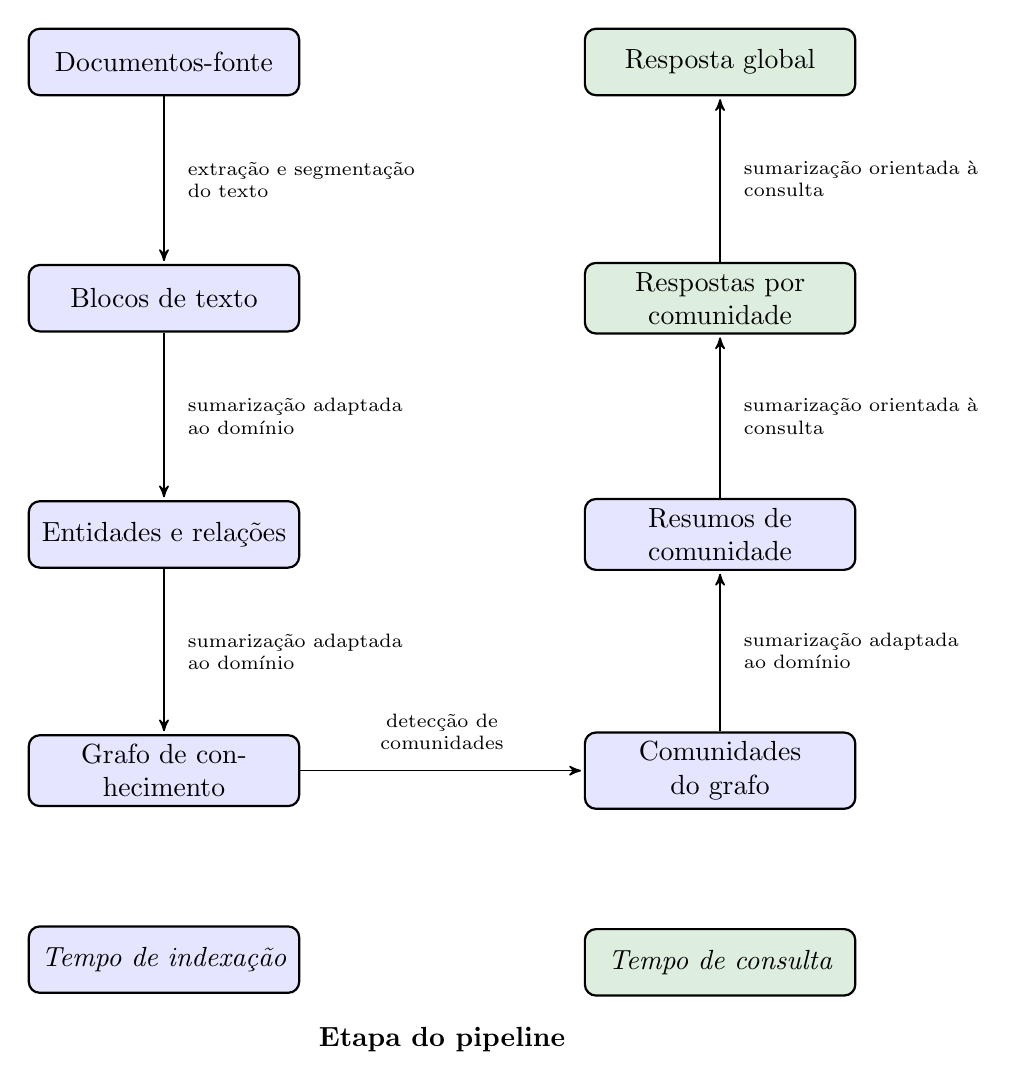
\begin{tikzpicture}[
        >=stealth', shorten >=1pt, semithick, node distance=3cm,
        index/.style={
            rectangle, draw=black, thick, fill=blue!10,
            text width=3.2cm, align=center, rounded corners, minimum height=2.4em
        },
        query/.style={
            rectangle, draw=black, thick, fill=ForestGreen!15,
            text width=3.2cm, align=center, rounded corners, minimum height=2.4em
        },
        elab/.style={midway, right=5pt, align=left, font=\scriptsize, text width=3cm},
        hlab/.style={midway, above=4pt, align=center, font=\scriptsize, text width=2.6cm}
      ]
      \node[index] (doc) {Documentos-fonte};
      \node[index, below of=doc] (chunks) {Blocos de texto};
      \node[index, below of=chunks] (er) {Entidades e relações};
      \node[index, below of=er] (kg) {Grafo de conhecimento};
      \node[index, right=3.6cm of kg] (comm) {Comunidades do grafo};
      \node[index, above of=comm] (csum) {Resumos de comunidade};
      \node[query, above of=csum] (cans) {Respostas por comunidade};
      \node[query, above of=cans] (global) {Resposta global};

      \draw[->] (doc)   -- (chunks) node[elab] {extração e segmentação do texto};
      \draw[->] (chunks) -- (er)    node[elab] {sumarização adaptada ao domínio};
      \draw[->] (er)    -- (kg)     node[elab] {sumarização adaptada ao domínio};
      \draw[->] (kg)    -- (comm)   node[hlab] {detecção de comunidades};
      \draw[->] (comm)  -- (csum)   node[elab] {sumarização adaptada ao domínio};
      \draw[->] (csum)  -- (cans)   node[elab] {sumarização orientada à consulta};
      \draw[->] (cans)  -- (global) node[elab] {sumarização orientada à consulta};

      \node[index, font=\itshape, below=1.5cm of kg]  (itime) {Tempo de indexação};
      \node[query, font=\itshape, below=1.5cm of comm] (qtime) {Tempo de consulta};
      \coordinate (legmid) at ($(itime)!0.5!(qtime)$);
      \node[font=\bfseries] at ([yshift=-1cm]legmid) {Etapa do pipeline};
    \end{tikzpicture}
    \caption[Pipeline do GraphRAG]{Pipeline do GraphRAG a partir de um índice de grafo derivado por LLM do texto dos documentos-fonte. O índice abrange nós (entidades) e arestas (relações), além de covariáveis opcionais, detectados, extraídos e resumidos por \textit{prompts} adaptados ao domínio dos dados. A detecção de comunidades (por exemplo, Leiden, \citealt{traag2019}) particiona o índice em grupos de elementos que o LLM resume em paralelo, tanto no tempo de indexação quanto no de consulta. A ``resposta global'' a uma consulta resulta de uma rodada final de sumarização orientada à consulta sobre todos os resumos de comunidade que reportam relevância para ela. Figura extraída de \citet{edge2024} e traduzida pelo autor para fins didáticos.}
    \label{fig:graphrag-pipeline}
\end{figure}

A detecção de comunidades no GraphRAG é feita pelo algoritmo de Leiden, proposto por \citet{traag2019} como aprimoramento do método de Louvain. Ambos buscam uma partição do grafo que maximize a modularidade, medida que compara a densidade de arestas dentro das comunidades com a que se esperaria em um grafo aleatório de mesmo grau. O método de Louvain, embora rápido e amplamente usado, pode produzir comunidades internamente mal conectadas, e até desconexas, situação em que um grupo rotulado como comunidade não forma, de fato, um subgrafo coeso. O Leiden acrescenta uma etapa de refinamento que garante que toda comunidade retornada seja internamente conectada, além de convergir para partições de melhor qualidade em menos iterações. O algoritmo é recursivo, no sentido de que, após encontrar uma partição, agrega cada comunidade em um supernó e repete o procedimento sobre o grafo agregado, o que gera uma hierarquia de partições em vez de uma partição única.

Essa recursão produz os níveis de comunidade (\textit{community levels}), níveis de granularidade da partição, exemplificados na Figura~\ref{fig:leiden-hierarquia}, que contrasta as comunidades detectadas em dois níveis sobre um conjunto de dados de exemplo. No nível mais agregado, identificado como L0, o grafo é dividido em poucas comunidades amplas, que correspondem a grandes temas do corpus. A cada nível subsequente, as comunidades do nível anterior são subdivididas, de modo que os níveis mais altos contêm muitas comunidades pequenas e tematicamente específicas. Os resumos acompanham essa gradação, pois níveis baixos geram resumos longos e abstratos, que sintetizam grandes porções do corpus, ao passo que níveis altos geram resumos curtos e concretos, próximos do texto de origem. \citet{edge2024} avaliaram condições de nível de comunidade denominadas C0 a C3 e observaram um compromisso, em que os níveis intermediários tendem a favorecer o embasamento factual das respostas, enquanto os níveis mais agregados favorecem a abrangência ao custo de especificidade. Para uma tarefa de classificação diagnóstica, em que a resposta é uma entre poucas categorias e depende de detalhes concretos do prontuário, a especificidade do contexto é prioritária, o que sugere preferência por níveis mais granulares.

\begin{figure}[htb]
    \centering
    \begin{tabular}{cc}
        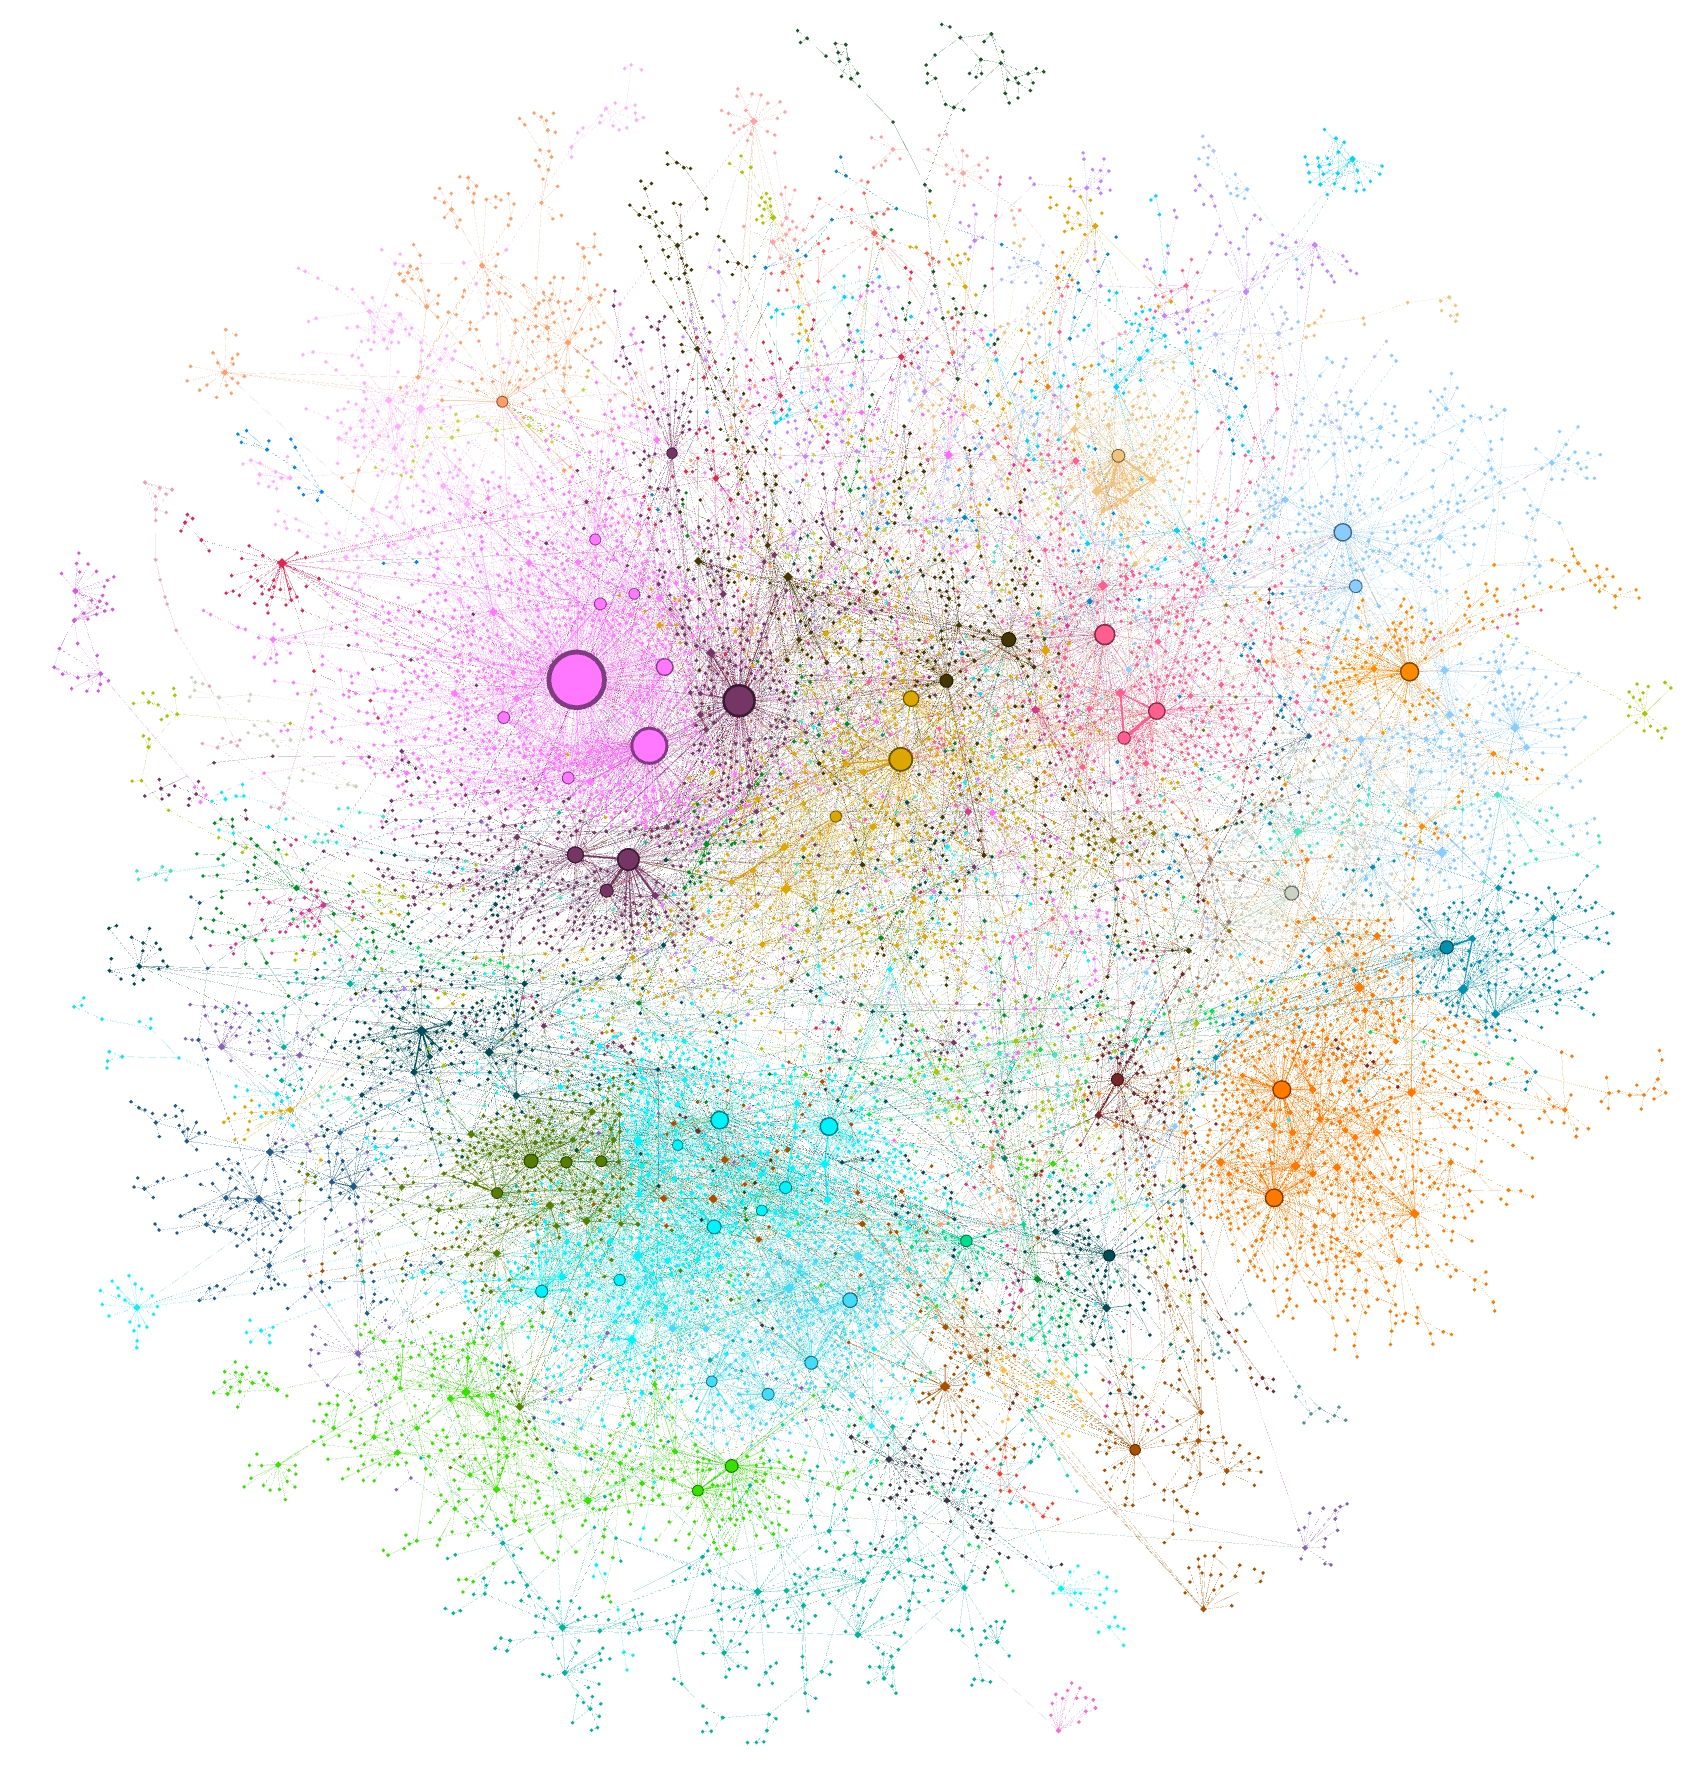
\includegraphics[width=0.47\textwidth]{Cap02/figuras/Level0Multihop.jpg} &
        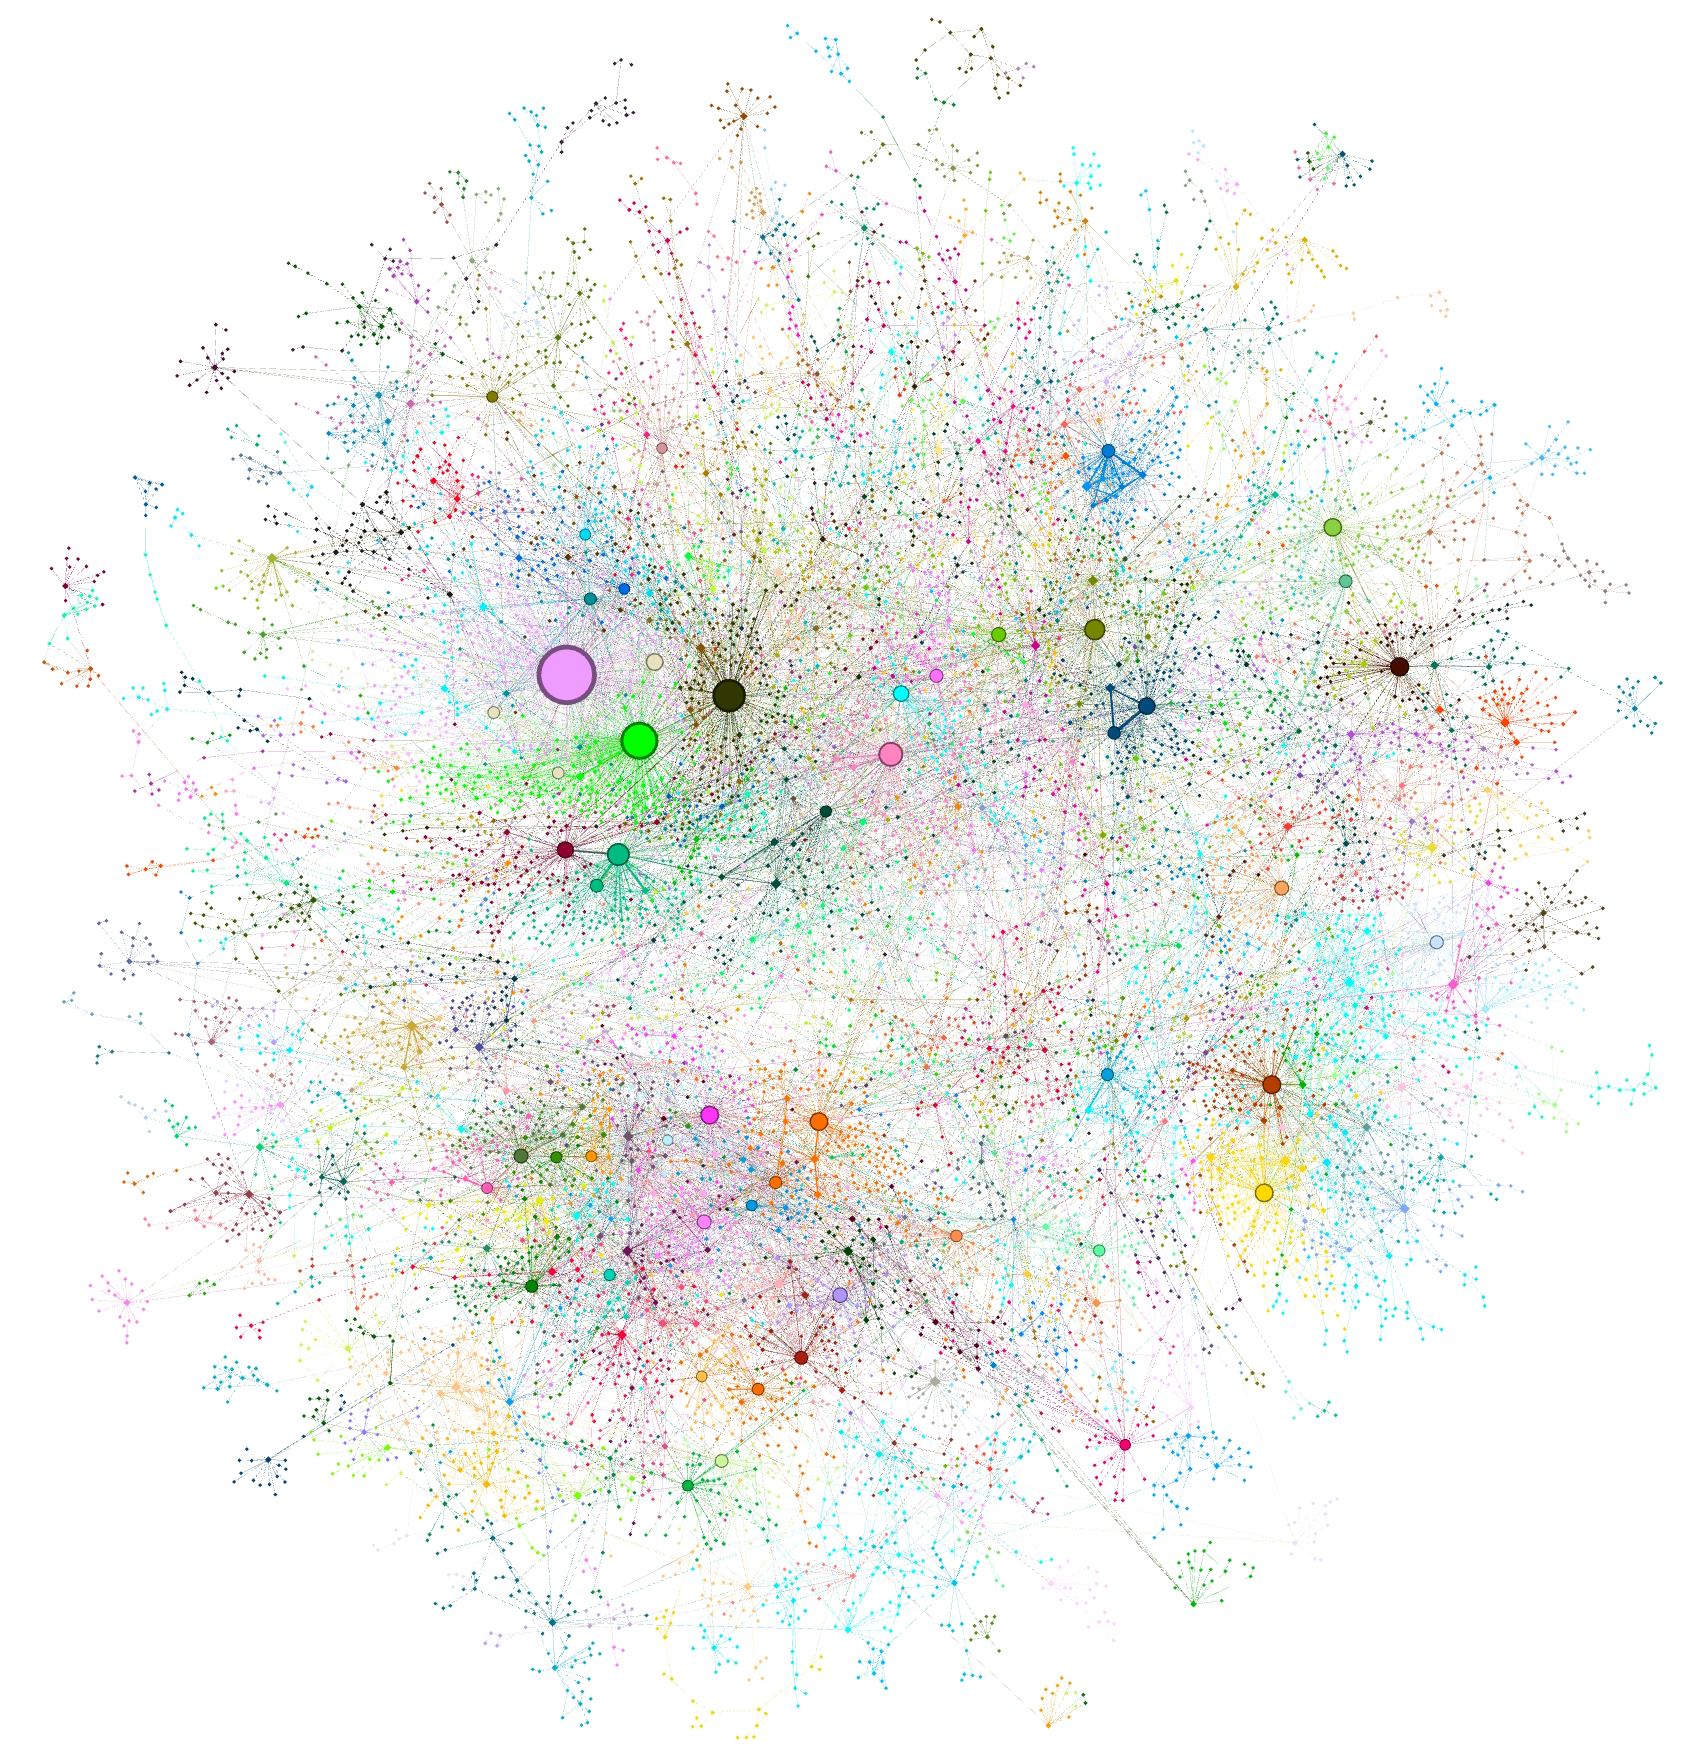
\includegraphics[width=0.47\textwidth]{Cap02/figuras/Level1Multihop.jpg} \\
        (a) Comunidades raiz no nível 0 & (b) Subcomunidades no nível 1
    \end{tabular}
    \caption[Comunidades detectadas pelo algoritmo de Leiden, em dois níveis]{Comunidades do grafo detectadas pelo algoritmo de Leiden \citep{traag2019} sobre um conjunto de dados de exemplo, tal como indexado. Os círculos representam nós de entidade, com tamanho proporcional ao grau, e o leiaute foi obtido com os algoritmos OpenORD e Force Atlas~2. As cores identificam comunidades de entidades em dois níveis do agrupamento hierárquico: (a) nível 0, correspondente à partição de modularidade máxima, e (b) nível 1, que revela a estrutura interna dessas comunidades de nível raiz. Níveis mais agregados produzem menos comunidades e resumos mais longos e abstratos; níveis mais granulares produzem muitas comunidades e resumos mais curtos e específicos. Figura extraída de \citet{edge2024}; legenda traduzida e condensada pelo autor para fins didáticos.}
    \label{fig:leiden-hierarquia}
\end{figure}

Na etapa de consulta, o GraphRAG oferece modos de busca distintos, que exploram o índice de maneiras diferentes e estão esquematizados na Figura~\ref{fig:modos-busca}. O modo \textit{basic} recupera diretamente as unidades de texto mais semelhantes à consulta, por similaridade vetorial, sem utilizar a estrutura do grafo, e equivale a um RAG convencional sobre o mesmo corpus. O modo \textit{local} parte da consulta para identificar as entidades mais relevantes no grafo e monta o contexto com essas entidades, sua vizinhança imediata, as relações que as conectam e as unidades de texto associadas, sendo adequado a perguntas centradas em entidades específicas. O modo \textit{global} destina-se a perguntas de sentido global e opera em \textit{map-reduce} sobre os resumos de comunidade de um dado nível, de modo que, na fase de \textit{map}, cada resumo é processado isoladamente para gerar respostas parciais com pontuação de utilidade e, na fase de \textit{reduce}, as respostas parciais mais úteis são combinadas em uma resposta final. O modo \textit{drift} combina as duas orientações em um processo iterativo, que inicia com uma consulta ampla aos resumos de comunidade e, a cada iteração, gera novas subperguntas e as refina com buscas locais, ampliando progressivamente o contexto. O modo \textit{drift} tende a produzir as respostas mais completas, ao custo de um número de chamadas ao LLM substancialmente maior que o dos demais modos.

\begin{figure}[htb]
\centering
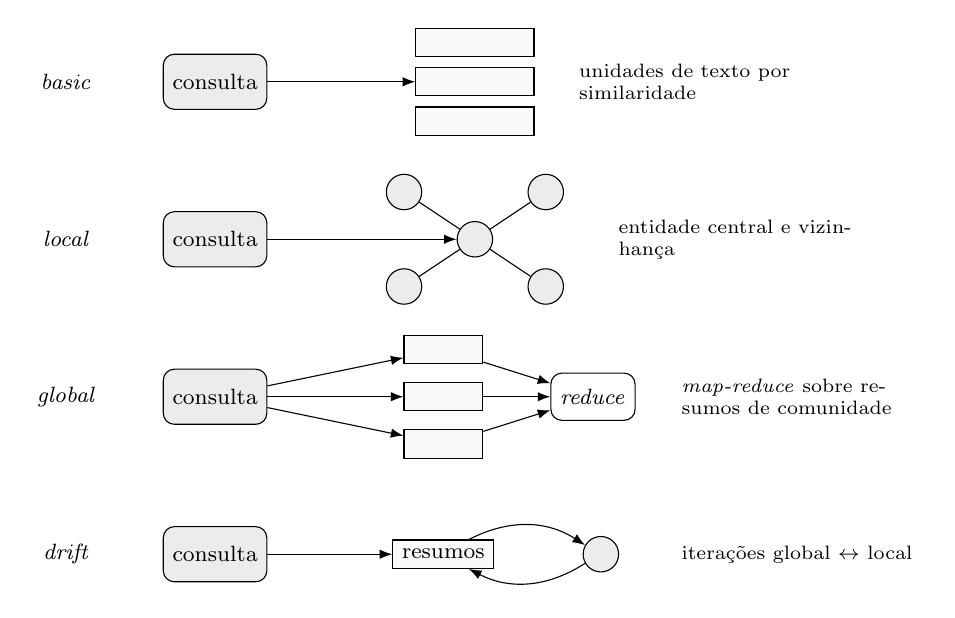
\begin{tikzpicture}[
  font=\footnotesize,
  q/.style={draw, rounded corners, fill=gray!15, minimum width=13mm, minimum height=7mm, align=center},
  lbl/.style={font=\footnotesize\itshape},
  ch/.style={draw, fill=gray!5, minimum width=15mm, minimum height=3.6mm},
  ent/.style={draw, circle, fill=gray!15, minimum size=4.5mm, inner sep=0},
  sm/.style={draw, fill=gray!5, minimum width=10mm, minimum height=3.6mm},
  note/.style={align=left, anchor=west, font=\scriptsize, text width=30mm},
  arr/.style={-{Latex[length=1.6mm]}}
]
\node[lbl] at (-3.3,0) {basic};
\node[q] (qb) at (-1.4,0) {consulta};
\node[ch] (b1) at (1.9,0.5) {};
\node[ch] (b2) at (1.9,0.0) {};
\node[ch] (b3) at (1.9,-0.5) {};
\draw[arr] (qb) -- (b2);
\node[note] at (3.1,0) {unidades de texto por similaridade};

\node[lbl] at (-3.3,-2) {local};
\node[q] (ql) at (-1.4,-2) {consulta};
\node[ent] (c) at (1.9,-2) {};
\node[ent] (n1) at (1.0,-1.4) {};
\node[ent] (n2) at (2.8,-1.4) {};
\node[ent] (n3) at (1.0,-2.6) {};
\node[ent] (n4) at (2.8,-2.6) {};
\draw (c)--(n1) (c)--(n2) (c)--(n3) (c)--(n4);
\draw[arr] (ql) -- (c);
\node[note] at (3.6,-2) {entidade central e vizinhança};

\node[lbl] at (-3.3,-4) {global};
\node[q] (qg) at (-1.4,-4) {consulta};
\node[sm] (s1) at (1.5,-3.4) {};
\node[sm] (s2) at (1.5,-4.0) {};
\node[sm] (s3) at (1.5,-4.6) {};
\node[draw, rounded corners, minimum height=6mm] (red) at (3.4,-4) {\textit{reduce}};
\draw[arr] (qg) -- (s1); \draw[arr] (qg) -- (s2); \draw[arr] (qg) -- (s3);
\draw[arr] (s1) -- (red); \draw[arr] (s2) -- (red); \draw[arr] (s3) -- (red);
\node[note] at (4.4,-4) {\textit{map-reduce} sobre resumos de comunidade};

\node[lbl] at (-3.3,-6) {drift};
\node[q] (qd) at (-1.4,-6) {consulta};
\node[sm] (ds) at (1.5,-6) {resumos};
\node[ent] (de) at (3.5,-6) {};
\draw[arr] (qd) -- (ds);
\draw[arr, bend left=30] (ds) to (de);
\draw[arr, bend left=30] (de) to (ds);
\node[note] at (4.4,-6) {iterações global $\leftrightarrow$ local};
\end{tikzpicture}
\caption[Modos de busca do GraphRAG]{Representação esquemática dos quatro modos de busca do Microsoft GraphRAG e da parcela do índice que cada um percorre.}
\label{fig:modos-busca}
\end{figure}

O pipeline padrão do GraphRAG utiliza \textit{prompts} de extração genéricos, concebidos para corpora de domínio aberto, que reconhecem tipos de entidade amplos como pessoa, organização e local. O GraphRAG permite substituir esses \textit{prompts} por versões adaptadas a um domínio, seja por um procedimento automático de ajuste a partir de amostras do corpus, seja por edição manual. A customização define os tipos de entidade pertinentes ao domínio e fornece exemplos \textit{few-shot} alinhados ao vocabulário efetivamente empregado nos documentos. Em hepatologia, isso significa instruir o modelo a extrair entidades como doença hepática, achado laboratorial, exame de imagem e complicação, e ilustrar a extração com trechos representativos de evoluções clínicas, de modo que o grafo resultante reflita as distinções relevantes para a pergunta de pesquisa.

O custo computacional é uma limitação prática incontornável do GraphRAG. A indexação exige uma chamada ao LLM por unidade de texto para a extração e uma chamada por comunidade para a geração de resumos, o que, em um corpus de centenas de documentos com milhares de comunidades, representa um volume elevado de inferências. A consulta também é onerosa, sobretudo nos modos \textit{global} e \textit{drift}, que multiplicam as chamadas ao percorrer resumos ou ao iterar. Esse custo, somado à latência, constitui barreira à adoção e motiva a avaliação criteriosa de quando o ganho de qualidade compensa o esforço adicional. Parte desse ganho, contudo, depende de como o modelo aproveita contextos longos, questão examinada a seguir.

\section{Contextos Longos, ``Lost in the Middle'' e Degradação da Atenção}\label{sec:contextos-longos}

O tamanho da janela de contexto dos LLMs cresceu de forma acelerada. Modelos amplamente usados por volta de 2020 operavam com poucos milhares de \textit{tokens}, ao passo que gerações recentes anunciam janelas de dezenas ou centenas de milhares de \textit{tokens}, e algumas ultrapassam a marca de um milhão. Esse aumento sugere, à primeira vista, que a limitação de espaço para a informação recuperada teria deixado de ser relevante, e que bastaria fornecer ao modelo todo o material potencialmente útil. A evidência empírica, contudo, mostra que a capacidade de utilizar o contexto não acompanha, na mesma proporção, a capacidade de recebê-lo.

\citet{liu2024} caracterizaram esse descompasso no fenômeno que denominaram \textit{lost in the middle}. Em seus experimentos, um documento contendo a resposta a uma pergunta era inserido em meio a vários documentos distratores, e sua posição na sequência era variada de forma sistemática, do início ao fim do contexto. O desempenho na recuperação da resposta não se manteve constante ao longo das posições, como seria de esperar se o modelo tratasse todo o contexto de maneira uniforme. Em vez disso, foi mais alto quando a informação relevante estava nas primeiras ou nas últimas posições e caiu de forma acentuada quando ela ocupava posições centrais, configurando uma curva em U, ilustrada de forma esquemática na Figura~\ref{fig:lost-middle}. O efeito foi observado em modelos distintos, inclusive naqueles projetados para contextos longos.

\begin{figure}[htb]
\centering
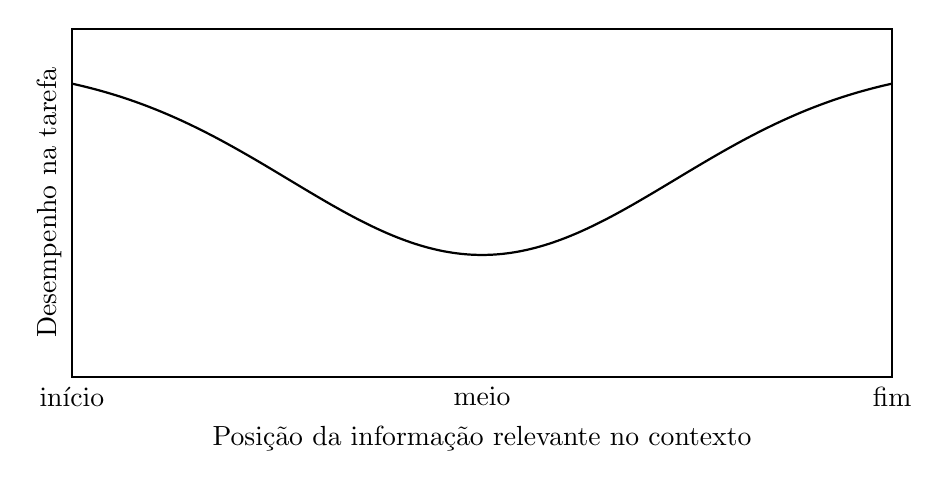
\begin{tikzpicture}
\begin{axis}[
    width=12cm, height=6cm,
    xlabel={Posição da informação relevante no contexto},
    ylabel={Desempenho na tarefa},
    xtick={1,10.5,20},
    xticklabels={início, meio, fim},
    ytick=\empty,
    ymin=0, ymax=1,
    xmin=1, xmax=20,
    domain=1:20, samples=100,
    thick, tick style={draw=none}
]
\addplot[smooth] {0.9 - 0.55*exp(-((x-10.5)^2)/40)};
\end{axis}
\end{tikzpicture}
\caption[Representação esquemática do fenômeno \textit{lost in the middle}]{Representação esquemática do fenômeno \textit{lost in the middle}. O desempenho é maior quando a informação relevante ocupa o início ou o fim do contexto e cai quando ela se encontra no meio, configurando a curva em U observada por \citet{liu2024}. A figura ilustra apenas o formato da relação, sem reproduzir valores específicos.}
\label{fig:lost-middle}
\end{figure}

O mecanismo por trás do fenômeno relaciona-se à forma como a atenção se distribui em sequências longas. À medida que o número de \textit{tokens} cresce, a massa de atenção que o modelo pode alocar dilui-se, e posições intermediárias tendem a receber menos peso. Soma-se a isso um viés de posição induzido pelo pré-treinamento, em que padrões de texto que privilegiam a informação no começo e no fecho de trechos são reforçados. A consequência prática é que a janela de contexto nominal, aquela que o modelo aceita sem erro, não equivale à janela efetivamente utilizável, dentro da qual a informação é de fato aproveitada. Alongar o contexto além desse ponto pode não trazer ganho, e até prejudicar, se deslocar informação útil para a região central.

Esse resultado tem implicação direta para os modos de busca do GraphRAG. O modo \textit{global} monta o contexto a partir dos resumos de várias comunidades, e o modo \textit{drift} acumula contexto ao longo de iterações sucessivas, de modo que ambos produzem \textit{prompts} substancialmente mais longos que os do modo \textit{local}, restrito à vizinhança de poucas entidades. Cabe a hipótese de que o ganho informacional de um contexto mais rico seja parcial ou integralmente anulado pela degradação da atenção sobre esse mesmo contexto. Se assim for, tem-se uma explicação plausível para observações recorrentes na literatura, em que abordagens de recuperação mais elaboradas não superam alternativas mais simples em tarefas nas quais a resposta depende de um trecho específico, e não de uma síntese ampla.

A mesma tensão aparece na escolha do nível de comunidade. Níveis mais agregados geram resumos mais longos e abstratos, que ampliam o volume de texto no contexto sem necessariamente aproximá-lo do detalhe que a pergunta exige. Níveis mais granulares geram resumos mais curtos e concretos, que produzem um contexto menor e mais focado. Retomando o compromisso discutido na Seção~\ref{sec:graphrag}, para uma tarefa de classificação diagnóstica a combinação de contexto enxuto e específico tende a ser preferível, tanto por alinhar-se à natureza da tarefa quanto por reduzir a exposição ao efeito \textit{lost in the middle}.

A literatura descreve estratégias para atenuar a degradação em contextos longos. A reordenação do contexto procura colocar os trechos mais promissores nas extremidades do \textit{prompt}, onde a atenção é mais confiável. O \textit{reranking} aplica um segundo modelo, mais preciso que a busca inicial, para ordenar os trechos recuperados por relevância antes da montagem. A compressão de contexto resume ou filtra os trechos para eliminar redundância e reduzir o comprimento total. A recuperação seletiva limita deliberadamente a quantidade de material fornecido, sob a premissa de que menos contexto, porém mais pertinente, produz respostas melhores. Essas técnicas convergem para um mesmo princípio, o de que a qualidade da seleção importa mais que a quantidade de texto.

Avaliar se um sistema de recuperação responde corretamente a uma pergunta com resposta bem definida exige, antes, um instrumental de métricas e testes estatísticos apropriado, tema da seção seguinte.

\section{Avaliação de Sistemas de Classificação}\label{sec:avaliacao}

A avaliação de um sistema que atribui rótulos a exemplos começa pela caracterização do problema de classificação. Na classificação binária há duas classes mutuamente exclusivas, como a presença ou a ausência de uma condição. Na classificação multiclasse há mais de duas classes exclusivas, e cada exemplo recebe exatamente um rótulo. Na classificação multirrótulo um exemplo pode receber vários rótulos simultâneos, situação adequada quando as categorias não se excluem. A escolha entre esses formatos depende da estrutura do domínio e da forma como a tarefa é definida.

O instrumento básico de análise é a matriz de confusão, que cruza os rótulos previstos com os verdadeiros. Dela derivam quatro contagens fundamentais: verdadeiros positivos (VP) e verdadeiros negativos (VN), em que a previsão coincide com a realidade, e falsos positivos (FP) e falsos negativos (FN), em que diverge. Em contexto diagnóstico, a assimetria entre os dois tipos de erro é relevante. Um falso negativo, deixar de identificar uma doença presente, pode retardar o tratamento e ter consequências graves; um falso positivo, atribuir uma doença ausente, gera investigação adicional e ansiedade, em geral com custo menor. Nenhuma métrica única captura essa assimetria, o que motiva a análise conjunta de várias.

A acurácia, proporção de previsões corretas sobre o total, é intuitiva mas enganosa sob desbalanceamento de classes, pois um classificador que sempre prevê a classe majoritária pode alcançar acurácia alta sem qualquer utilidade. A precisão mede, entre os exemplos previstos como pertencentes a uma classe, a fração que de fato pertence; a revocação mede, entre os exemplos que pertencem à classe, a fração recuperada. O F1-score é a média harmônica entre precisão e revocação, e penaliza o desequilíbrio entre as duas. Em problemas com várias classes, o F1 macro calcula a média aritmética dos F1 por classe, atribuindo o mesmo peso a todas, enquanto o F1 ponderado pondera cada classe por seu suporte, o número de exemplos, o que faz as classes raras influírem pouco no valor final.

A concordância bruta entre previsão e referência ignora que parte das coincidências ocorreria por acaso. O coeficiente \textit{kappa} de \citet{cohen1960} corrige esse efeito, comparando a concordância observada com a esperada sob atribuição aleatória, e assume valor 1 na concordância perfeita e próximo de 0 quando ela não supera o acaso. \citet{landis_koch1977} propuseram uma escala de interpretação amplamente adotada, que classifica valores até 0,20 como concordância leve, de 0,21 a 0,40 como razoável, de 0,41 a 0,60 como moderada, de 0,61 a 0,80 como substancial e acima de 0,80 como quase perfeita.

O coeficiente de correlação de \citet{matthews1975} resume a matriz de confusão em um único número entre $-1$ e $1$, calculado a partir das quatro contagens de forma balanceada. Sua principal vantagem é a robustez sob desbalanceamento severo, pois só assume valor alto quando o classificador acerta bem tanto os positivos quanto os negativos, em termos relativos ao tamanho de cada grupo. Por isso é preferível ao F1 quando há classes de suporte muito baixo, situação em que o F1 pode oscilar bruscamente com poucos acertos ou erros e transmitir uma impressão distorcida do desempenho.

Estimativas pontuais de métricas ganham em interpretabilidade quando acompanhadas de intervalos de confiança. O método \textit{bootstrap} constrói esses intervalos por reamostragem com reposição do conjunto de teste, gerando muitas amostras do mesmo tamanho, recalculando a métrica em cada uma e tomando a distribuição resultante como base para os limites do intervalo. O procedimento não exige pressupostos sobre a forma da distribuição da métrica e adapta-se bem a amostras pequenas, comuns em domínios especializados.

A comparação entre sistemas e a investigação de hipóteses explicativas requerem testes estatísticos. Testes paramétricos, como a análise de variância, pressupõem que os dados seguem determinada distribuição, em geral a normal, e perdem validade quando esse pressuposto não se sustenta, o que é frequente com métricas limitadas a intervalos e amostras reduzidas. Testes não-paramétricos dispensam esse pressuposto. Para comparar dois sistemas sobre as mesmas observações pareadas, quando a variável de interesse é binária, o teste de \citet{mcnemar1947} avalia se a proporção de casos em que um sistema acerta e o outro erra é simétrica entre as duas direções possíveis, sem exigir pressuposto sobre a distribuição subjacente; sua versão exata calcula o p-valor diretamente pela distribuição binomial, adequada mesmo com poucas discordâncias. Para comparar uma variável quantitativa entre dois grupos independentes, sem pressupor normalidade, o teste U de \citet{mann_whitney1947} compara as distribuições por meio dos postos dos valores combinados dos dois grupos. Para comparar a proporção de uma variável categórica entre dois ou mais grupos, o teste qui-quadrado de \citet{pearson1900} compara as frequências observadas às esperadas sob a hipótese de independência entre grupo e variável. Em todos os casos, adota-se nível de significância convencional de 5\%.

Todos esses instrumentos pressupõem a existência de um gabarito confiável contra o qual medir o acerto, e a forma de obtê-lo é assunto da subseção seguinte.

\subsection{Ground Truth, Anotação e Avaliação por LLM}\label{sec:ground-truth}

Chama-se \textit{ground truth} o conjunto de rótulos de referência considerados corretos, contra os quais as saídas de um sistema são comparadas. Distingue-se o padrão-ouro, produzido por anotação humana especializada, do padrão-prata, gerado por processo automático ou semiautomático, como regras ou um modelo auxiliar. O padrão-ouro oferece maior confiabilidade ao custo de esforço humano; o padrão-prata amplia a escala ao custo de ruído, e costuma servir para tarefas em que um erro ocasional de rótulo é tolerável.

Em domínios especializados, a anotação manual é onerosa porque depende de profissionais escassos e exige tempo por caso. Uma estratégia para viabilizá-la é a amostragem estratificada, que seleciona um subconjunto do corpus preservando a proporção de características relevantes, como as classes de interesse, de modo que um número menor de itens anotados ainda represente a distribuição do todo e sustente estimativas válidas.

Quando mais de um anotador rotula os mesmos itens, mede-se a concordância entre anotadores, com coeficientes como o \textit{kappa} discutido acima. Uma concordância alta indica que a tarefa de anotação é bem definida e que os rótulos são reproduzíveis, o que valida o \textit{ground truth}; uma concordância baixa sinaliza ambiguidade na definição das classes ou nos critérios, e recomenda revisão antes do uso.

Uma alternativa à anotação humana é o uso de um LLM como avaliador, abordagem conhecida como \textit{LLM-as-Judge}. Na modalidade \textit{reference-based}, o modelo julga uma resposta tendo à disposição uma resposta de referência; na modalidade \textit{reference-free}, avalia atributos como coerência, completude ou fundamentação sem gabarito. \textit{Frameworks} como o RAGAS \citep{es2023} operacionalizam esse tipo de avaliação para sistemas de recuperação, com métricas automáticas de fidelidade ao contexto e de pertinência da resposta.

A avaliação por LLM carrega vieses documentados \citep{zheng2023}. O viés de posição faz o modelo preferir de forma sistemática a alternativa apresentada em primeiro lugar em comparações par a par. O viés de verbosidade o inclina a favorecer respostas mais longas, independentemente de sua correção. Há ainda sensibilidade a variações na formulação do \textit{prompt} de avaliação, que alteram o resultado sem mudança de conteúdo. Auditorias recentes sugerem que parte dos ganhos relatados para sistemas GraphRAG avaliados dessa maneira pode ser atribuível a esses artefatos, e não a mérito real, e recomendam a randomização da ordem de apresentação das respostas como mitigação \textbf{[VERIFICAR REFERÊNCIA: auditoria recente sobre avaliação de GraphRAG por LLM]}.

Em tarefas de classificação, nas quais a resposta é uma categoria verificável, a anotação humana especializada tem vantagem sobre a avaliação automática por LLM. Ela permite calcular métricas objetivas, como as discutidas acima, e aplicar testes de hipótese formais, além de não reintroduzir, no processo de avaliação, o mesmo tipo de modelo cujo desempenho se quer medir. Por isso este trabalho adota \textit{ground truth} anotado por especialista como base de avaliação.

\label{sec:estrutura-causal}As oito condições hepáticas avaliadas não são independentes entre si, e sua estrutura causal condiciona a formulação da tarefa. A esteatose hepática, a hepatite B e a hepatite C são causas frequentes de dano hepático crônico que pode evoluir para cirrose. A cirrose e a esquistossomose hepatoesplênica são causas de hipertensão portal, respectivamente nas formas cirrótica e não cirrótica. A hemorragia digestiva alta e a peritonite bacteriana espontânea são descompensações da doença hepática de base, associadas à hipertensão portal e à cirrose avançada. Um mesmo paciente pode, portanto, apresentar várias dessas condições encadeadas, o que motiva a formulação da tarefa como classificação multirrótulo: a cada prontuário associa-se o subconjunto das oito condições documentadas como presentes, em vez de uma única categoria. Ainda assim, a estrutura causal exige cuidado na distinção entre doença de base e complicação, de modo que a fronteira entre classes permanece um ponto sensível da avaliação, discutido na definição do critério de presença clara na Seção~\ref{sec:met-prompt}.

Definidos os fundamentos, o próximo capítulo detalha a metodologia adotada para construir e avaliar os sistemas.

\cleardoublepage
% % % % % % % % % % % % % % % % % % % % % % % % % % % %
\chapter{Metodologia}\label{cap:metodologia}

Este capítulo descreve o percurso metodológico adotado para atingir o objetivo geral enunciado no Capítulo~\ref{cap:introducao}, o de desenvolver e avaliar uma abordagem baseada em GraphRAG para a extração de informações clínicas de prontuários eletrônicos de pacientes hepatopatas. Para tornar essa avaliação mensurável, a extração foi formulada como uma tarefa de classificação multirrótulo: dado o texto de um prontuário, o sistema deve indicar quais, dentre oito doenças hepáticas definidas previamente, estão claramente documentadas como presentes no paciente. A pergunta que orienta o trabalho não se limita a verificar se o sistema acerta, mas busca identificar qual configuração de busca do Microsoft GraphRAG apresenta melhor desempenho nesse tipo de extração clínica e por quais razões.

As seções seguem a ordem cronológica de execução do trabalho, sintetizada na Figura~\ref{fig:met-visao-geral}. Inicialmente, apresentam-se os dados e as classes-alvo, seguidos da construção da amostra avaliada e de seus rótulos de referência. Em seguida, descrevem-se a construção do grafo de conhecimento, os modos de busca e os sistemas comparados, o \textit{prompt} de extração, o modelo de linguagem e a infraestrutura de execução. Por fim, detalham-se a conversão das respostas em classes, as métricas e os testes estatísticos, a análise qualitativa de erros e as limitações metodológicas. Os valores de desempenho obtidos são apresentados no capítulo de resultados; neste capítulo constam apenas os números que fundamentam decisões de projeto.

\begin{figure}[!htbp]
\centering
\resizebox{\textwidth}{!}{% Arquitetura do sistema avaliado, em quatro painéis.
% Gramática visual inspirada na figura de visão geral de Xonto-RAG
% (Wang et al., 2026): painéis numerados com fundo pastel, mini-grafos e
% setas largas entre etapas; cores da paleta da tese (estilo-visual.tex).
\begin{tikzpicture}[
  x=1cm, y=1cm, font=\sffamily\footnotesize,
  painel/.style={rounded corners=9pt, line width=0.8pt, draw=black!35},
  titulo/.style={anchor=west, font=\rmfamily\bfseries\normalsize, inner sep=0pt},
  num/.style={circle, draw=black!75, line width=0.8pt, inner sep=1.2pt, minimum size=5mm, font=\rmfamily\bfseries\normalsize},
  caixa/.style={rounded corners=3pt, line width=0.6pt, align=center, inner sep=3pt, fill=white},
  seta/.style={-{Latex[length=1.8mm]}, line width=0.7pt, black!70},
  setao/.style={single arrow, shape border uses incircle, draw=black!45, fill=black!25, minimum height=6.5mm, minimum width=7mm, single arrow head extend=1.3mm, inner sep=0pt},
  no/.style={circle, minimum size=2.6mm, inner sep=0pt, line width=0.6pt},
  na/.style={no, fill=vAzul!45, draw=vAzul!80!black},
  nl/.style={no, fill=vLaranja!50, draw=vLaranja!80!black},
  nv/.style={no, fill=vVerde!45, draw=vVerde!80!black},
  aresta/.style={line width=0.6pt, black!45},
  rotulo/.style={font=\sffamily\scriptsize, text=black!65}
]
\def\PW{7.55}\def\PH{4.55}\def\GX{0.70}\def\GY{0.50}

% ======================================================= fundos dos painéis
\path[painel, fill=vAmbar!14]  (0,0) rectangle (\PW,-\PH);
\path[painel, fill=vAzul!11]   (\PW+\GX,0) rectangle (2*\PW+\GX,-\PH);
\path[painel, fill=vVerde!12]  (0,-\PH-\GY) rectangle (\PW,-2*\PH-\GY);
\path[painel, fill=vRoxo!9]    (\PW+\GX,-\PH-\GY) rectangle (2*\PW+\GX,-2*\PH-\GY);

% setas largas entre painéis
\node[setao] at ({\PW+\GX/2},{-\PH/2}) {};
\node[setao, shape border rotate=225, minimum height=5.5mm] at ({\PW+\GX/2},{-\PH-\GY/2}) {};
\node[setao] at ({\PW+\GX/2},{-1.5*\PH-\GY}) {};

% ============================== 1. Construção da amostra e dos rótulos
\begin{scope}
\node[num] at (0.42,-0.42) {1};
\node[titulo] at (0.82,-0.42) {Construção da amostra};
% funil: faixas cada vez mais estreitas
\foreach \i/\w/\cor/\rot in {
    0/6.7/vNeutro!85/{\faDatabase\ \ Corpus: 3.757 prontuários, 6.405 atendimentos},
    1/5.9/vAmbar!30/{\faFilter\ \ Triagem por expressões regulares},
    2/5.1/vAmbar!45/{\faRobot\ \ Triagem por LLM},
    3/4.3/vAmbar!62/{\faUserMd\ \ Anotação manual (segunda opinião)}}{
  \pgfmathsetmacro{\yt}{-0.85-\i*0.60}
  \pgfmathsetmacro{\yb}{\yt-0.53}
  \pgfmathsetmacro{\wb}{\w-0.8}
  \path[fill=\cor, draw=white, line width=1pt]
    ({\PW/2-\w/2},\yt) -- ({\PW/2+\w/2},\yt) -- ({\PW/2+\wb/2},\yb) -- ({\PW/2-\wb/2},\yb) -- cycle;
  \node[font=\sffamily\scriptsize] at ({\PW/2},{(\yt+\yb)/2}) {\rot};
}
\draw[seta] ({\PW/2},-3.22) -- ({\PW/2},-3.47);
\node[caixa, draw=vAmbar!80!black, text width=6.2cm, font=\sffamily\scriptsize] at ({\PW/2},-3.92)
  {\textbf{537 prontuários} com rótulos de referência\\[1pt]
   \tikz[baseline=-0.6ex]{\foreach \k/\c in {0/vAzul,1/vVerde,2/vLaranja,3/vAmbar,4/vRoxo,5/vVermelho,6/vTeal,7/vCinza}{\fill[\c] (\k*0.32,0) circle (1.1mm);}}
   \ \ oito doenças (multirrótulo)};
\end{scope}

% ======================================================= 2. Indexação (GraphRAG)
\begin{scope}[xshift={(\PW+\GX)*1cm}]
\node[num] at (0.42,-0.42) {2};
\node[titulo] at (0.82,-0.42) {Indexação pelo GraphRAG};
\node[caixa, draw=vAzul!75!black, text width=1.95cm, font=\sffamily\scriptsize] (pt)  at (1.25,-1.15) {Ajuste de\\\textit{prompts}};
\node[caixa, draw=vAzul!75!black, text width=1.95cm, font=\sffamily\scriptsize] (seg) at (3.78,-1.15) {Segmentação\\5.541 unidades};
\node[caixa, draw=vAzul!75!black, text width=1.95cm, font=\sffamily\scriptsize] (ext) at (6.30,-1.15) {Entidades e\\relações (LLM)};
\draw[seta] (pt) -- (seg); \draw[seta] (seg) -- (ext);
% mini-grafo com três comunidades (achatado na vertical)
\begin{scope}[shift={(0.35,-1.90)}, yscale=0.60]
  \draw[vAzul!70, dashed, line width=0.5pt, rounded corners=5pt] (0.05,-0.15) rectangle (1.35,-1.55);
  \draw[vLaranja!80, dashed, line width=0.5pt, rounded corners=5pt] (1.55,-0.15) rectangle (2.95,-1.40);
  \draw[vVerde!80, dashed, line width=0.5pt, rounded corners=5pt] (0.70,-1.75) rectangle (2.45,-2.85);
  \node[na] (a1) at (0.35,-0.45) {}; \node[na] (a2) at (1.05,-0.50) {}; \node[na] (a3) at (0.45,-1.20) {}; \node[na] (a4) at (1.10,-1.25) {};
  \node[nl] (b1) at (1.90,-0.45) {}; \node[nl] (b2) at (2.65,-0.55) {}; \node[nl] (b3) at (2.25,-1.10) {};
  \node[nv] (c1) at (1.00,-2.10) {}; \node[nv] (c2) at (1.75,-2.05) {}; \node[nv] (c3) at (1.35,-2.55) {}; \node[nv] (c4) at (2.15,-2.55) {};
  \draw[aresta] (a1)--(a2) (a1)--(a3) (a2)--(a4) (a3)--(a4) (a2)--(a3) (b1)--(b2) (b2)--(b3) (b1)--(b3)
                (c1)--(c2) (c1)--(c3) (c2)--(c4) (c3)--(c4) (c2)--(c3);
  \draw[aresta, dashed, black!35] (a2)--(b1) (a4)--(c1) (b3)--(c2);
\end{scope}
\node[align=center, rotulo] at (1.85,-4.08) {Grafo: 26.966 entidades,\\88.347 relações};
\draw[seta] (ext.south) -- ++(0,-0.20) -| (2.45,-1.97);
% hierarquia de Leiden
\begin{scope}[shift={(4.75,-1.95)}]
  \node[rotulo, anchor=east] at (0.05,0) {nível 0};
  \node[rotulo, anchor=east] at (0.05,-0.58) {nível 1};
  \node[rotulo, anchor=east] at (0.05,-1.16) {nível 2};
  \node[no, fill=vNeutro, draw=black!55, minimum size=3.4mm] (r) at (1.35,0) {};
  \node[na, minimum size=3mm] (h1) at (0.65,-0.58) {}; \node[nl, minimum size=3mm] (h2) at (1.35,-0.58) {}; \node[nv, minimum size=3mm] (h3) at (2.05,-0.58) {};
  \foreach \k/\x/\s in {1/0.40/na, 2/0.90/na, 3/1.20/nl, 4/1.55/nl, 5/1.85/nv, 6/2.30/nv}{\node[\s, minimum size=2.2mm] (t\k) at (\x,-1.16) {};}
  \draw[aresta] (r)--(h1) (r)--(h2) (r)--(h3) (h1)--(t1) (h1)--(t2) (h2)--(t3) (h2)--(t4) (h3)--(t5) (h3)--(t6);
  \node[rotulo] at (1.35,-1.45) {$\vdots$ até o nível 6};
\end{scope}
\node[align=center, rotulo] at (5.80,-4.08) {Comunidades de Leiden\\e resumos de comunidade};
\draw[seta] (3.32,-2.75) -- (3.82,-2.75);
\end{scope}

% ======================================================= 3. Consulta (S1 a S8)
\begin{scope}[yshift={-(\PH+\GY)*1cm}]
\node[num] at (0.42,-0.42) {3};
\node[titulo] at (0.82,-0.42) {Consulta: sistemas S1 a S8};
\node[caixa, draw=vVerde!75!black, text width=1.95cm, font=\sffamily\scriptsize] (pr) at (1.22,-1.55) {\faFileMedical\ \ Prontuário\\{\tiny até 8.000 caracteres}};
\node[caixa, draw=vVerde!75!black, text width=1.95cm, font=\sffamily\scriptsize] (pp) at (1.22,-2.60) {\faAlignLeft\ \ \textit{Prompt}\\{\tiny de extração}};
% grade modo x nível
\begin{scope}[shift={(2.62,-0.90)}]
  \node[rotulo] at (2.175,0.02) {nível de comunidade};
  \node[font=\sffamily\scriptsize\bfseries] at (1.75,-0.28) {1};
  \node[font=\sffamily\scriptsize\bfseries] at (2.60,-0.28) {2};
  \foreach \j/\m/\c/\a/\b/\op in {1/basic/modoBasic/S1/S2/1, 2/local/modoLocal/S3/S4/1, 3/global/modoGlobal/S5/S6/0.4, 4/drift/modoDrift/S7/S8/1}{
    \pgfmathsetmacro{\y}{-0.28-\j*0.47}
    \node[anchor=west, inner sep=0pt] at (0,\y) {\chip{\c}\textit{\m}};
    \node[caixa, draw=\c!80!black, fill=\c!20, minimum width=8mm, inner sep=2pt, opacity=\op, text opacity=\op] at (1.75,\y) {\a};
    \node[caixa, draw=\c!80!black, fill=\c!20, minimum width=8mm, inner sep=2pt, opacity=\op, text opacity=\op] at (2.60,\y) {\b};
  }
\end{scope}
\draw[line width=0.7pt, black!70] (pr.east) -| (2.40,-2.08);
\draw[line width=0.7pt, black!70] (pp.east) -| (2.40,-2.08);
\draw[seta] (2.40,-2.08) -- (2.60,-2.08);
\node[caixa, draw=vVerde!75!black, text width=1.0cm] (llm) at (6.60,-2.03) {{\Large\faRobot}\\[1pt] LLM};
\node[font=\ttfamily\tiny, text=black!70, anchor=north] at (llm.south) {gpt-oss-120b};
\draw[seta] (5.64,-2.03) -- (llm.west);
\node[fill=vVermelho!75, text=white, rounded corners=2pt, align=left, inner sep=3.5pt, font=\sffamily\scriptsize] at ({\PW/2},-3.97)
  {\textbf{Pergunta:} quais das oito doenças hepáticas estão\\documentadas como presentes neste prontuário?};
\end{scope}

% ======================================================= 4. Extração e avaliação
\begin{scope}[xshift={(\PW+\GX)*1cm}, yshift={-(\PH+\GY)*1cm}]
\node[num] at (0.42,-0.42) {4};
\node[titulo] at (0.82,-0.42) {Extração e avaliação};
\node[caixa, draw=black!45, text width=3.25cm, align=left, font=\ttfamily\tiny] (resp) at (1.95,-1.62)
  {{\sffamily\scriptsize\bfseries Resposta do modelo}\\[2pt] <RESPOSTA>\\ Cirrose hepática: ``\ldots''\\ Hipertensão portal: ``\ldots''\\ </RESPOSTA>};
\node[caixa, draw=vRoxo!75!black, text width=2.75cm, font=\sffamily\scriptsize] (parser) at (5.75,-1.62)
  {\faCogs\ \textbf{\textit{Parser}}\\determinístico\\[1pt]{\tiny\color{black!65}nomes canônicos e negação}};
\draw[seta] (resp) -- (parser);
\node[caixa, draw=vRoxo!75!black, text width=6.75cm, align=left, font=\sffamily\scriptsize] (aval) at ({\PW/2},-3.45)
  {\textbf{Doenças previstas} $\times$ \textbf{rótulos de referência}\\[1pt]
   \faChartBar\ \ métricas multirrótulo (EM, P, R, F1)\\
   \faFlask\ \ hipóteses H1 a H4 sobre o modo \textit{drift}\\
   \faSearch\ \ análise qualitativa de erros e do grafo};
\draw[seta] (parser.south) -- (parser.south |- aval.north);
\end{scope}
\end{tikzpicture}
}
\caption[Arquitetura do sistema avaliado]{Arquitetura do sistema avaliado: (1) construção da amostra (Seção~\ref{sec:met-amostra}); (2) indexação pelo GraphRAG (Seção~\ref{sec:met-grafo}); (3) consulta pelos sistemas S1 a S8, com S5 e S6 esmaecidos por não terem sido concluídos (Seção~\ref{sec:met-sistemas}); e (4) extração e avaliação.}
\label{fig:met-visao-geral}
\par\smallskip{\footnotesize Fonte: elaborado pelo autor.}
\end{figure}

\section{Dados}\label{sec:met-dados}

Os dados utilizados são prontuários eletrônicos reais do ambulatório de hepatologia do Hospital Universitário da Universidade Federal de Alagoas (HU-UFAL), em Maceió, Alagoas.
O corpus reúne 3.757 prontuários únicos, que totalizam 6.405 registros de atendimento. Cada prontuário corresponde à concatenação, em ordem cronológica, de todas as evoluções clínicas de um mesmo paciente, com os atendimentos individuais delimitados pelo marcador textual \texttt{-{}-{}- Atendimento -{}-{}-}. O conteúdo é predominantemente texto livre e exibe as características discutidas na Seção~\ref{sec:prontuarios}, como abreviações não padronizadas, estilo telegráfico e menções frequentes a hipóteses negadas ou não confirmadas.

Quanto aos aspectos éticos, os prontuários foram anonimizados antes de qualquer uso neste trabalho.
% TODO: descrever o procedimento de anonimização (ferramenta, categorias de dados removidas, verificação do resultado).
Essa etapa é particularmente relevante porque, nas consultas da rodada final, o texto anonimizado dos prontuários foi enviado a um provedor externo de inferência, acessado por meio de uma interface de programação de aplicações (API), conforme a Seção~\ref{sec:met-modelo}, e não processado exclusivamente em ambiente local. A anonimização prévia constitui, portanto, a principal salvaguarda adotada em relação ao tratamento de dados pessoais sensíveis disciplinado pela Lei Geral de Proteção de Dados Pessoais (LGPD).
% TODO: citar o texto da LGPD (não há entrada no .bib).
% TODO: informar parecer do CEP/CAAE.

\section{Definição das classes-alvo}\label{sec:met-classes}

As oito classes avaliadas são cirrose hepática, esquistossomose, hepatite B, hepatite C, esteatose hepática, hipertensão portal, hemorragia digestiva alta (HDA) e peritonite bacteriana espontânea (PBE). Essas condições não foram selecionadas por critério estatístico nem descobertas de forma exploratória no texto: foram definidas \textit{a priori} por uma profissional de hepatologia, com base em sua relevância clínica no contexto do ambulatório de origem dos dados.

\label{sec:estrutura-causal}As oito condições não são independentes entre si, e sua estrutura causal condiciona a formulação da tarefa. A esteatose hepática, a hepatite B e a hepatite C são causas frequentes de dano hepático crônico que pode evoluir para cirrose. A cirrose e a esquistossomose hepatoesplênica são causas de hipertensão portal, respectivamente nas formas cirrótica e não cirrótica. A hemorragia digestiva alta e a peritonite bacteriana espontânea são descompensações da doença hepática de base, associadas à hipertensão portal e à cirrose avançada. Um mesmo paciente pode, portanto, apresentar várias dessas condições encadeadas, o que motiva a formulação da tarefa como classificação multirrótulo: a cada prontuário associa-se o subconjunto das oito condições documentadas como presentes, em vez de uma única categoria. Ainda assim, a estrutura causal exige cuidado na distinção entre doença de base e complicação, de modo que a fronteira entre classes permanece um ponto sensível da avaliação, discutido na definição do critério de presença clara na Seção~\ref{sec:met-prompt}.

A lista fixa de classes é o ponto de partida de todo o pipeline. Tanto a triagem de prontuários candidatos, descrita na Seção~\ref{sec:met-amostra}, quanto o \textit{prompt} de extração, apresentado na Seção~\ref{sec:met-prompt}, foram construídos em torno exatamente dessas oito categorias. Definidas as classes, o passo seguinte consistiu em selecionar os prontuários a avaliar e estabelecer, para cada um deles, o conjunto correto de doenças.

\section{Construção da amostra e dos rótulos de referência}\label{sec:met-amostra}

Os experimentos foram conduzidos sobre um conjunto de 537 prontuários extraído do corpus de 3.757. Esse conjunto não constitui amostra aleatória: foi construído por um funil de três etapas, representado no painel 1 da Figura~\ref{fig:met-visao-geral}. A escolha decorre do fato de que uma amostra aleatória simples teria prevalência baixa demais de cada uma das oito doenças, com número de casos positivos por classe insuficiente para uma avaliação multirrótulo. O funil contorna esse problema ao enriquecer a amostra com prontuários que plausivelmente mencionam as condições de interesse.

A primeira etapa consistiu em uma triagem por expressões regulares sobre o texto bruto de todo o corpus, em busca de menções às oito doenças-alvo. Um teste manual preliminar mostrou que uma busca ingênua pelos termos produzia falsos positivos sistemáticos, o que motivou quatro correções:
\begin{enumerate}
    \item desconsiderar a colisão entre a sigla HDA da doença-alvo e o cabeçalho de seção ``H.D.A.'' (história da doença atual), que respondia sozinha por cerca de 73\% dos falsos positivos de HDA antes da correção;
    \item descartar menções explicitamente negadas, marcadas por termos como ``nega'', ``ausente'' e ``descartado'';
    \item descartar menções marcadas por incerteza (\textit{hedges}), como ``?'', ``a esclarecer'', ``suspeita de'' e ``epidemiologia positiva'', que indicam risco, e não achado positivo;
    \item descartar menções em contexto histórico ou já resolvido, como ``passado de'' e ``história de'', exceto quando a condição é o motivo do atendimento atual.
\end{enumerate}
A saída dessa etapa foi uma lista de prontuários candidatos, isto é, que mencionam ao menos uma das oito doenças de forma textualmente plausível.

A segunda etapa submeteu os candidatos a uma triagem por LLM. Para cada prontuário, realizou-se uma chamada direta ao modelo, sem indexação nem recuperação, com uma pergunta curta que solicitava confirmação binária (sim ou não) para cada doença candidata. O objetivo foi reduzir o volume de falsos positivos antes da revisão humana, a etapa mais onerosa do funil. As chamadas foram executadas em paralelo e de forma retomável, o que permitiu reiniciar o processamento a partir do ponto de interrupção.
% TODO: informar o modelo de linguagem usado na triagem por LLM.

A terceira etapa foi a anotação manual, denominada no projeto ``segunda opinião'': uma revisão humana dos candidatos que passaram pelas etapas anteriores, que produziu o rótulo definitivo de cada prontuário. Esse conjunto constitui o \textit{ground truth} do trabalho, isto é, o conjunto de rótulos considerados corretos contra os quais as saídas do sistema são comparadas, e é referido daqui em diante como rótulos de referência.
% TODO: informar quantos anotadores participaram, sua formação e se houve medida de concordância entre anotadores (por exemplo, kappa de Cohen). A Seção 2.7 afirma que o trabalho adota ground truth "anotado por especialista"; confirmar.

Os números disponíveis confirmam que o funil molda a composição da amostra final. Em uma rodada específica de expansão da amostra, foram registrados 396 prontuários candidatos. Dos 68 prontuários que terminaram rotulados sem nenhuma das oito doenças, 43 (63\%) pertencem a esse grupo de candidatos, ou seja, foram sinalizados pela triagem textual, mas a revisão por LLM ou manual concluiu que a menção não correspondia a diagnóstico presente, seja por negação, por incerteza ou por contexto histórico não capturados pelas expressões regulares. O grupo sem doença, portanto, não é um grupo de controle aleatório: resulta, em parte substancial, da própria filtragem de falsos positivos.

A Tabela~\ref{tab:met-distribuicao} apresenta a distribuição final das classes. Por se tratar de classificação multirrótulo, os percentuais não somam 100\%, e cada paciente apresenta, em média, 1,49 doenças confirmadas. Duas ressalvas decorrem dessa distribuição. A primeira refere-se à PBE, com apenas 2 casos positivos em toda a amostra: qualquer métrica calculada sobre essa classe deve ser lida como ruído estatístico, e não como indicação de desempenho, pois uma única previsão a mais ou a menos altera o valor por completo. A segunda refere-se à prevalência observada, que é artefato do critério de seleção enriquecido e não deve ser extrapolada como estimativa epidemiológica da população atendida no ambulatório.

\begin{table}[!htbp]
\centering
\caption[Distribuição das classes na amostra de 537 prontuários]{Distribuição das classes na amostra de 537 prontuários. Como a classificação é multirrótulo, os percentuais não somam 100\%.}
\label{tab:met-distribuicao}
\begin{tabular}{lrl}
\toprule
Doença & Pacientes & \% da amostra \\
\midrule
Hipertensão portal & 201 & \barcell{vTeal}{0.9350}{37,4} \\
Esteatose hepática & 156 & \barcell{vTeal}{0.7275}{29,1} \\
Cirrose hepática & 152 & \barcell{vTeal}{0.7075}{28,3} \\
Esquistossomose & 95 & \barcell{vTeal}{0.4425}{17,7} \\
Hepatite B & 90 & \barcell{vTeal}{0.4200}{16,8} \\
Hepatite C & 67 & \barcell{vTeal}{0.3125}{12,5} \\
Hemorragia digestiva alta & 36 & \barcell{vTeal}{0.1675}{6,7} \\
Peritonite bacteriana espontânea & 2 & \barcell{vTeal}{0.0100}{0,4} \\
\midrule
Nenhuma das oito doenças & 68 & \barcell{vCinza}{0.3175}{12,7} \\
\bottomrule
\end{tabular}
\par\smallskip{\footnotesize Fonte: elaborado pelo autor.}
\end{table}

\section{Construção do grafo de conhecimento}\label{sec:met-grafo}

Paralelamente à construção da amostra, o corpus foi indexado pelo GraphRAG. O índice foi construído uma única vez, antes de qualquer consulta, segundo o pipeline de indexação descrito na Seção~\ref{sec:graphrag} e representado no painel 2 da Figura~\ref{fig:met-visao-geral}. Esta seção não retoma o funcionamento geral de cada etapa, mas registra como ela foi aplicada ao corpus e quais estruturas resultaram.
% TODO: confirmar se o índice cobre o corpus completo de 3.757 prontuários ou apenas a amostra de 537.
% TODO: informar o modelo de linguagem e o modelo de embeddings usados na indexação, o tamanho das unidades de texto e a sobreposição entre elas.

Antes da indexação, executou-se o procedimento automático de ajuste de \textit{prompts} (\textit{prompt tuning}) oferecido pelo próprio GraphRAG, que gera \textit{prompts} de extração adaptados ao domínio a partir de uma amostra do corpus. A diferença mais relevante entre as versões genérica e ajustada está no \textit{prompt} de extração de entidades e relações. A versão genérica exige uma lista fixa de tipos de entidade, tipicamente categorias amplas de propósito geral, como pessoa, organização e local; a versão ajustada não fixa os tipos e solicita ao modelo que sugira categorias, tão gerais quanto possível, a partir do próprio conteúdo.

Em decorrência desse ajuste, os tipos de entidade observados no grafo final são específicos do domínio clínico, como \texttt{CONDICAO\_CLINICA}, \texttt{EXAME}, \texttt{EXAME\_LABORATORIAL}, \texttt{MEDICAMENTO}, \texttt{PROCEDIMENTO}, \texttt{SINAL\_CLINICO}, \texttt{ÓRGÃO}, \texttt{HÁBITO} e \texttt{PROTOCOLO}, em vez de categorias genéricas sem relação com o domínio. Como todos os modos de busca dependem, em graus diferentes, da qualidade do grafo, esse ajuste é pré-requisito comum a todos os sistemas avaliados.

O cuidado com essa etapa tem respaldo na literatura. \citet{ye2026} relatam que o pipeline padrão do GraphRAG, aplicado a prontuários eletrônicos, produz granularidade excessiva, que degrada significativamente a recuperação: o \textit{prompt} original identificava cada parâmetro laboratorial como entidade independente, o que provocava uma proliferação acentuada de entidades. Os autores contornaram o problema com \textit{prompts} customizados para o domínio, que incluem a exigência de que cada registro contenha exatamente uma entidade do tipo paciente, à qual se vinculam diagnósticos, medicamentos e exames. Neste trabalho, o ajuste empregado foi o procedimento automático do próprio GraphRAG, sem regras explícitas dessa natureza, o que tem consequências para a estrutura do grafo discutidas na Seção~\ref{sec:res-grafos}.

A indexação propriamente dita compreendeu quatro etapas. Na segmentação (\textit{chunking}), o corpus foi dividido em 5.541 unidades de texto (\textit{text units}), unidade mínima à qual se vinculam tanto as entidades extraídas quanto os documentos de origem. Na extração de entidades e relações, um LLM leu cada unidade de texto e identificou entidades, como diagnósticos, exames, medicamentos, procedimentos e sinais clínicos, bem como as relações entre elas, o que resultou em um grafo com 26.966 entidades e 88.347 relações.

A detecção de comunidades empregou a implementação hierárquica do algoritmo de Leiden \citep{traag2019} disponível na biblioteca graspologic, que particiona o grafo em grupos de nós densamente interconectados, maximizando a modularidade. O caráter recursivo do algoritmo, discutido na Seção~\ref{sec:graphrag}, faz com que as comunidades de um nível sejam subdivididas no nível seguinte, o que gerou uma hierarquia de 7 níveis, numerados de 0, o mais amplo, a 6, o mais granular. Cabe registrar que essa partição é puramente topológica: depende apenas de quais entidades estão conectadas e com que peso, sem nenhuma etapa semântica no agrupamento em si.

Por fim, na geração de resumos de comunidade (\textit{community reports}), um LLM produziu, para cada comunidade, um resumo textual a partir das entidades, das relações e dos trechos de texto associados a ela. Esses resumos constituem o material consultado pelos modos \textit{global} e \textit{drift}. O índice resultante é comum a todos os sistemas; o que os distingue é a forma como cada modo de busca o percorre, tema da seção seguinte.

\section{Modos de busca e sistemas avaliados}\label{sec:met-sistemas}

Com o índice construído, cada consulta, composta pelo texto de um prontuário e pelo \textit{prompt} de extração, pode ser respondida por quatro modos de busca, cujo funcionamento geral foi apresentado na Seção~\ref{sec:graphrag} e na Figura~\ref{fig:modos-busca}. No modo \textit{basic}, não há uso estruturado do grafo: como o texto do prontuário já está embutido na própria consulta, o modo opera essencialmente como uma chamada direta ao modelo de linguagem, sem recuperação adicional a partir do índice.
% TODO: conferir com a Seção 2.5, que descreve o basic como recuperação de unidades de texto por similaridade vetorial; se houve recuperação de unidades de texto nesta configuração, ajustar o texto.
O modo \textit{local} recupera contexto centrado nas entidades relevantes para a consulta, com suas relações diretas e as unidades de texto de origem. Seu desempenho depende diretamente do que foi extraído na indexação, pois uma entidade que não foi criada nessa etapa não pode ser recuperada depois.

O modo \textit{global} percorre os resumos de comunidade, seja de um nível fixo da hierarquia, seja, quando a seleção dinâmica de comunidades (\textit{dynamic community selection}) está ativa, navegando a hierarquia de forma adaptativa a partir do nível 0 e avaliando a relevância de cada comunidade antes de decidir se desce mais um nível. O modo \textit{drift} combina as orientações local e global de forma iterativa: realiza uma varredura inicial (\textit{primer}), gera perguntas de acompanhamento (\textit{follow-ups}) com base no que já foi encontrado, configuradas para até 6 por consulta, e executa buscas locais específicas para cada uma delas, refinando a resposta em múltiplas rodadas.

\subsection{Desenho experimental}\label{sec:met-desenho}

O cruzamento dos quatro modos de busca com dois níveis de comunidade, 1 e 2, produz os oito sistemas apresentados na Tabela~\ref{tab:met-sistemas}. O desenho prevê que todos sejam avaliados lado a lado sobre os mesmos 537 prontuários, com o mesmo \textit{prompt} de extração e o mesmo modelo de linguagem, de forma que o modo de busca seja a principal variável isolada na comparação, e o nível de comunidade, a variável secundária. Os sistemas S5 e S6, correspondentes ao modo \textit{global}, integram o desenho, mas não foram concluídos de forma confiável com o modelo adotado, pelos motivos expostos na Seção~\ref{sec:met-limitacoes}; a comparação efetiva restringe-se, por isso, aos seis sistemas restantes.
% TODO: esclarecer se S5 e S6 usaram seleção dinâmica de comunidades e como o nível 1 ou 2 se aplica nesse caso.

\begin{table}[!htbp]
\centering
\caption[Sistemas avaliados, por modo de busca e nível de comunidade]{Sistemas avaliados, definidos pelo cruzamento entre modo de busca e nível de comunidade.}
\label{tab:met-sistemas}
\begin{tabular}{lcc}
\toprule
Modo de busca & Nível 1 & Nível 2 \\
\midrule
\chip{modoBasic}\textit{basic}  & S1 & S2 \\
\chip{modoLocal}\textit{local}  & S3 & S4 \\
\chip{modoGlobal}\textit{global} & {\color{black!45}S5} & {\color{black!45}S6} \\
\chip{modoDrift}\textit{drift}  & S7 & S8 \\
\bottomrule
\end{tabular}
\par\smallskip{\footnotesize Fonte: elaborado pelo autor. Em cinza, os sistemas não concluídos de forma confiável (Seção~\ref{sec:met-limitacoes}).}
\end{table}

Uma consequência do desenho merece registro. Como o modo \textit{basic} não utiliza a estrutura do grafo, o nível de comunidade não interfere na montagem do seu contexto, de modo que S1 e S2 correspondem, na prática, a duas execuções independentes da mesma configuração. Esse par oferece, assim, uma referência da variação entre execuções atribuível ao próprio modelo, útil para interpretar as diferenças entre níveis observadas nos demais modos.
% TODO: confirmar que, na configuração usada, o parâmetro de nível de comunidade não altera o comportamento do modo basic.

\subsection{Escolha dos níveis de comunidade}\label{sec:met-niveis}

A hierarquia produzida pelo algoritmo de Leiden possui 7 níveis, e a Tabela~\ref{tab:met-niveis} mostra como o número e o tamanho das comunidades variam ao longo dela. O nível 0 foi descartado por conter apenas 46 comunidades, com tamanho médio de 543,6 entidades. A distribuição é fortemente assimétrica, com mediana de apenas 5 entidades, o que indica que poucas comunidades muito grandes concentram a maior parte do grafo. Utilizá-lo agregaria, em uma mesma comunidade, informação de muitos pacientes e de temas heterogêneos, o que é incompatível com uma tarefa que exige granularidade por paciente. Esse perfil é característico das hierarquias produzidas pelo algoritmo de Leiden em grafos de conhecimento, que tendem a ser dominadas por poucas comunidades grandes e cujos tamanhos variam amplamente entre níveis, o que torna irregular a qualidade dos resumos gerados a partir delas \citep{hossain2026}. Os mesmos autores defendem comunidades de tamanho limitado e que preservem a conectividade interna como as mais adequadas à recuperação e à sumarização, critério com o qual é compatível a escolha descrita a seguir.

\begin{table}[!htbp]
\centering
\caption[Número e tamanho das comunidades por nível da hierarquia]{Número e tamanho das comunidades, em entidades, em cada nível da hierarquia do índice. Os níveis 1 e 2 foram os adotados nos sistemas avaliados.}
\label{tab:met-niveis}
\begin{tabular}{crrr}
\toprule
Nível & Comunidades & Tamanho médio & Tamanho mediano \\
\midrule
0 & 46    & 543,6 & 5 \\
\rowcolor{linhaDestaque}1 & 501   & 49,7  & 5 \\
\rowcolor{linhaDestaque}2 & 1.475 & 16,1  & 6 \\
3 & 1.959 & 9,7   & 4 \\
4 & 591   & 15,9  & 3 \\
5 & 60    & 85,1  & 6 \\
6 & 7     & 577,3 & 2 \\
\bottomrule
\end{tabular}
\par\smallskip{\footnotesize Fonte: elaborado pelo autor a partir do índice construído. Em destaque, os níveis adotados.}
\end{table}

Os níveis mais profundos foram descartados por razões opostas. O nível 3 apresenta o maior número de comunidades da hierarquia (1.959), com mediana de 4 entidades, o que amplia o custo computacional dos modos que percorrem comunidades inteiras, como o \textit{global}, e aumenta o risco de separar entidades clinicamente relacionadas em comunidades distintas. Nos níveis 4 a 6, o número de comunidades volta a diminuir, enquanto a relação entre tamanho médio e mediano se torna irregular, sem ganho evidente de especificidade. Os níveis 1 e 2, com 501 e 1.475 comunidades e medianas de 5 e 6 entidades, ocupam a faixa intermediária da hierarquia: são finos o suficiente para separar temas clínicos distintos, sem a fragmentação e o custo dos níveis mais profundos, em consonância com o compromisso entre abrangência e especificidade discutido na Seção~\ref{sec:graphrag}.

Avaliar os dois níveis, em vez de escolher um único \textit{a priori}, permite verificar empiricamente se a escolha do nível afeta o desempenho. Essa verificação foi feita por meio do teste estatístico descrito a seguir.

\subsection{Comparação entre níveis: teste de McNemar exato}\label{sec:met-mcnemar}

Para verificar se a escolha entre os níveis 1 e 2 produz diferença estatisticamente significativa, aplicou-se, para cada modo de busca, o teste de McNemar exato \citep{mcnemar1947} sobre o acerto exato por paciente (\textit{exact match}, definido na Seção~\ref{sec:met-metricas}).
O teste é pareado porque os mesmos pacientes são avaliados nos dois níveis de um mesmo modo. Para cada paciente, registra-se se o conjunto de doenças previsto coincide integralmente com o de referência em cada nível, e apenas os pares discordantes entram na estatística: $b$ denota o número de pacientes acertados somente no nível 1, e $c$, o número de pacientes acertados somente no nível 2.

Sob a hipótese nula de que os dois níveis têm a mesma probabilidade de acerto, cada par discordante tem igual chance de favorecer qualquer um deles, de modo que $b$ segue distribuição binomial com $n = b + c$ tentativas e probabilidade $1/2$. A versão exata do teste calcula o p-valor bilateral diretamente dessa distribuição, conforme a Equação~\eqref{eq:mcnemar}, sem recorrer à aproximação pela distribuição qui-quadrado, o que a torna adequada mesmo quando o número de discordâncias é pequeno. Adotou-se nível de significância de 5\%.
% TODO: no modo drift o teste foi aplicado a 531 pacientes, e não a 537; explicar a diferença (por exemplo, pacientes sem resposta válida em um dos níveis), se confirmado.
\begin{equation}
p = \min\left(1,\; 2\sum_{k=0}^{\min(b,c)} \binom{n}{k}\left(\frac{1}{2}\right)^{n}\right)
\label{eq:mcnemar}
\end{equation}

\section{\texorpdfstring{\textit{Prompt}}{Prompt} de extração}\label{sec:met-prompt}

O \textit{prompt} enviado em cada consulta passou por três versões ao longo do trabalho, cada uma voltada a corrigir um problema concreto identificado na análise de erros das versões anteriores. As três compartilham uma estrutura comum. Todas solicitam explicitamente que o modelo indique quais das oito doenças estão claramente documentadas como presentes, entendendo-se por isso diagnóstico explícito, exame confirmatório ou estadiamento formal. Todas truncam o texto do prontuário em 8.000 caracteres e exigem que a resposta seja delimitada pelas marcas \texttt{<RESPOSTA>} e \texttt{</RESPOSTA>}, com uma doença por linha no formato ``nome da doença: trecho que confirma''.

Integram também a estrutura comum duas regras de interpretação. A regra de negação estabelece que resultados registrados como ``NR'' ou ``negativo'' indicam ausência, e não presença, da condição. A regra temporal, específica para HDA e PBE, determina que essas condições só sejam consideradas quando ativas ou recentes, e não quando se tratar de episódio antigo já resolvido.

A Tabela~\ref{tab:met-prompts} resume a evolução das versões. A versão 2 acrescentou a exigência de que o nome da doença na resposta seja exatamente um dos oito nomes canônicos da lista, sem variação nem sinônimo, mudança motivada pela dificuldade do \textit{parser} (Seção~\ref{sec:met-parser}) em reconhecer as variações livres de nomenclatura produzidas com a primeira versão.

\begin{table}[!htbp]
\centering
\caption[Evolução do \textit{prompt} de extração]{Evolução do \textit{prompt} de extração e problema que motivou cada versão.}
\label{tab:met-prompts}
\begin{tabular}{cp{7.0cm}p{5.6cm}}
\toprule
Versão & Alteração introduzida & Problema que a motivou \\
\midrule
1 & \raggedright Estrutura comum: critério de presença clara, truncamento em 8.000 caracteres, resposta delimitada, regra de negação e regra temporal para HDA e PBE & \raggedright Versão inicial \tabularnewline
2 & \raggedright Nome da doença restrito aos oito nomes canônicos, sem sinônimos & \raggedright Variações livres de nomenclatura não reconhecidas pelo \textit{parser} \tabularnewline
3 & \raggedright Bloco com três confusões recorrentes (HDA e sangramento baixo; hipertensão portal e arterial; escores não escritos e achados sem relação hepática) e reforço contra a listagem por risco ou epidemiologia & \raggedright Erros recorrentes identificados na análise qualitativa \tabularnewline
\bottomrule
\end{tabular}
\par\smallskip{\footnotesize Fonte: elaborado pelo autor.}
\end{table}

A versão 3 acrescentou um bloco explícito com três confusões recorrentes identificadas na análise qualitativa dos erros. A primeira é a distinção anatômica entre hemorragia digestiva alta e sangramento baixo ou retal, como o decorrente de hemorroida ou fissura anal. A segunda é a distinção entre hipertensão portal e hipertensão arterial, termos que compartilham apenas a palavra ``hipertensão''. A terceira é a proibição de citar ou inferir escores de estadiamento, como Child-Pugh, MELD e FIB-4, que não estejam literalmente escritos no texto, bem como de usar como evidência achados de órgãos ou sistemas sem relação hepática direta, salvo quando o texto estabelece essa relação explicitamente. A versão 3 reforçou, ainda, a proibição de listar uma doença apenas por menção de risco, probabilidade ou epidemiologia, sem diagnóstico confirmado.

A versão 3 é a versão final do \textit{prompt} e foi empregada nos sistemas S1 a S4 na rodada definitiva. Uma vez fixado o \textit{prompt}, as consultas passam a depender do modelo de linguagem que as responde e da infraestrutura que as executa, descritos a seguir.
% TODO: informar qual versão do prompt foi usada em S7 e S8 (drift) na rodada final; a fonte registra apenas que a versão 3 foi "testada isoladamente no drift".

\section{Modelo de linguagem e infraestrutura de execução}\label{sec:met-modelo}

A rodada que produziu os resultados reportados no Capítulo~\ref{cap:resultados} -- os oito sistemas sobre os 537 prontuários -- utilizou o modelo \texttt{inclusionai/ling-2.6-flash}, acessado pelo serviço de roteamento OpenRouter. Trata-se de um modelo instrucional, sem etapa de raciocínio expandido, o que mantém a latência baixa e previsível: a duração média observada no modo \textit{drift} (o mais custoso, por encadear múltiplas chamadas) foi de 214 segundos por consulta, com mediana de 190 segundos.
% TODO: informar temperatura e demais parâmetros de decodificação, se fixados, e o provedor/custo por token do ling-2.6-flash na rodada final.

Houve, posteriormente, uma tentativa de migrar todos os sistemas para \texttt{inclusionai/ling-3.0-flash}, um modelo de raciocínio híbrido (\textit{hybrid reasoning}) da mesma família, com o objetivo de uniformizar o modelo entre todas as comparações. Essa tentativa, no entanto, não foi concluída: cobriu apenas os modos \textit{basic} e \textit{local} (S1 a S4), e os modos \textit{global} e \textit{drift} não chegaram a produzir um conjunto de resultados confiável nessa migração, pelos motivos discutidos na Seção~\ref{sec:met-limitacoes}. Os resultados do Capítulo~\ref{cap:resultados}, portanto, referem-se integralmente à rodada em \texttt{ling-2.6-flash}, e não à tentativa de migração para \texttt{ling-3.0-flash}.
% TODO: revisar esta seção à luz da tentativa de migração: decidir se os
% resultados parciais em ling-3.0-flash (S1-S4) devem ser citados no
% capítulo de resultados como comparação complementar, e registrar
% explicitamente que a tentativa de validação do prompt de HDA (Seção
% \ref{sec:res-validacao-hda}) foi conduzida sobre ling-3.0-flash, não sobre
% o modelo da rodada final -- a comparação ali deve ser lida como um
% experimento novo num modelo diferente e mais lento, não como réplica
% exata da condição de S7/S8.

O modelo \texttt{ling-3.0-flash} é um modelo de raciocínio híbrido, que gera \textit{tokens} de raciocínio não exibidos antes de produzir a resposta final, acessado pelo mesmo serviço de roteamento, com inferência realizada pelo provedor Novita ao custo de US\$~0,021 por milhão de \textit{tokens} de entrada e US\$~0,063 por milhão de \textit{tokens} de saída. Esse comportamento aumenta de forma substancial o custo e a latência e torna esta última muito variável: uma mesma consulta pode levar de segundos a horas, de forma pouco previsível -- mesmo no modo \textit{basic} (S1), o mais simples, a duração média observada na tentativa de migração subiu para 566 segundos, cerca de 25 vezes a média equivalente em \texttt{ling-2.6-flash} no mesmo modo. O esforço de raciocínio foi configurado no nível baixo. A execução com esse modelo e com esse provedor exigiu, contudo, três ajustes no código do GraphRAG, descritos nos parágrafos seguintes.

O primeiro ajuste refere-se ao formato de resposta estruturada. O GraphRAG original força respostas no formato de objeto JSON (\textit{JavaScript Object Notation}) nas etapas de \textit{map} do modo \textit{global} e de \textit{primer} do modo \textit{drift}, configuração recusada por provedores que aceitam apenas respostas validadas por esquema JSON. Uma primeira correção removeu essa exigência de todas as chamadas ao LLM, mas afetou também a etapa de avaliação de relevância de comunidades, usada pela seleção dinâmica, e provocou centenas de respostas malformadas por consulta. A correção final restringiu a remoção, por meio da inspeção da pilha de chamadas, aos módulos que de fato apresentavam o problema, preservando o comportamento original no restante do sistema.

O segundo ajuste diz respeito ao esforço de raciocínio. O parâmetro correspondente na configuração do GraphRAG não produz efeito quando a chamada passa pela biblioteca intermediária litellm até o OpenRouter, pois é descartado sem aviso. Por isso, foi necessário injetar o parâmetro diretamente no corpo de cada requisição de geração, no formato reconhecido pelo OpenRouter, para que o esforço baixo fosse efetivamente aplicado.

O terceiro ajuste foi a paralelização das consultas, uma vez que a execução original, sequencial, era inviável em escala com um modelo de raciocínio lento. A concorrência foi ajustada empiricamente por modo de busca, a partir da medição do uso de memória por processo, já que o limite efetivo era a memória da máquina local, e não o limite de requisições da API. Adotaram-se seis processos simultâneos no modo \textit{basic}, três no modo \textit{local}, que consome cerca de 1,3~GB por processo, quase o dobro do \textit{basic}, e dois nos modos \textit{global} e \textit{drift}.

\section{Extração da resposta}\label{sec:met-parser}

Embora delimitada por marcas, a resposta de cada consulta é texto livre e precisa ser convertida em um conjunto de classes positivas. Essa conversão foi feita por um \textit{parser} determinístico, aplicado de forma idêntica a todos os sistemas e em todas as análises, a fim de garantir a comparabilidade dos resultados. O \textit{parser} percorre o trecho delimitado linha a linha em busca dos oito nomes canônicos e de variações mapeadas, com correspondência restrita a palavras inteiras. Uma linha só é contada como predição positiva se não contiver nenhum marcador de negação de uma lista auditada e corrigida ao longo do trabalho, que inclui, entre outros, ``ausente'', ``descartado'', ``negativo'', ``não confirmado'', ``nega'' e ``NR''.

Uma exceção a essa regra foi introduzida após uma auditoria de falsos negativos. Menções a carga viral negativa ou indetectável do vírus da hepatite B (HBV), registrada como PCR-HBV ou HBV-DNA, não são tratadas como negação da doença, pois indicam tratamento supressor bem-sucedido em paciente já diagnosticado com hepatite B crônica: a terapia da hepatite B é supressora, e não curativa, e o paciente permanece com a doença mesmo com carga viral indetectável. A exceção não se estende à hepatite C, cujo tratamento com antivirais de ação direta é frequentemente curativo, de modo que um PCR negativo para o vírus da hepatite C (HCV) após o tratamento costuma indicar doença de fato resolvida. Um teste realizado antes de restringir a correção à hepatite B confirmou que aplicá-la também à hepatite C produzia falsos positivos.

\section{Métricas e análise estatística}\label{sec:met-metricas}

Para cada sistema e cada classe $c$, os pares formados por paciente e doença foram classificados em verdadeiros positivos ($\mathrm{VP}_c$), falsos positivos ($\mathrm{FP}_c$), falsos negativos ($\mathrm{FN}_c$) e verdadeiros negativos ($\mathrm{VN}_c$), por comparação entre o conjunto previsto e os rótulos de referência. A partir dessas contagens, calcularam-se a precisão, a revocação (\textit{recall}) e o F1 de cada classe, conforme as definições da Seção~\ref{sec:avaliacao}. Essas métricas foram agregadas de duas formas, sendo $C$ o conjunto das oito classes. A agregação macro calcula a média simples entre as classes, atribuindo a todas o mesmo peso independentemente da prevalência, conforme a Equação~\eqref{eq:f1-macro}, e de forma análoga para a precisão e a revocação:
\begin{equation}
\mathrm{F1}_{\text{macro}} = \frac{1}{|C|}\sum_{c \in C} \mathrm{F1}_c .
\label{eq:f1-macro}
\end{equation}

A agregação micro, por sua vez, soma as contagens de todas as classes antes da divisão, ponderando implicitamente cada classe por sua frequência, conforme a Equação~\eqref{eq:pr-micro}; o $\mathrm{F1}_{\text{micro}}$ é a média harmônica entre $P_{\text{micro}}$ e $R_{\text{micro}}$:
\begin{equation}
P_{\text{micro}} = \frac{\sum_{c \in C} \mathrm{VP}_c}{\sum_{c \in C} \left(\mathrm{VP}_c + \mathrm{FP}_c\right)},
\qquad
R_{\text{micro}} = \frac{\sum_{c \in C} \mathrm{VP}_c}{\sum_{c \in C} \left(\mathrm{VP}_c + \mathrm{FN}_c\right)} .
\label{eq:pr-micro}
\end{equation}

Além das métricas por classe, adotou-se a acurácia de correspondência exata (\textit{exact match}, também denominada \textit{subset accuracy}), definida na Equação~\eqref{eq:em} como a proporção de pacientes cujo conjunto previsto $\hat{Y}_i$ é idêntico ao conjunto de referência $Y_i$, em que $N$ é o número de pacientes e $\mathbf{1}[\cdot]$ é a função indicadora. Trata-se da métrica mais rigorosa do trabalho, pois um único erro em qualquer das oito classes invalida o acerto do paciente inteiro, e é também a variável comparada no teste de McNemar (Seção~\ref{sec:met-mcnemar}).
\begin{equation}
\mathrm{EM} = \frac{1}{N}\sum_{i=1}^{N} \mathbf{1}\left[\hat{Y}_i = Y_i\right]
\label{eq:em}
\end{equation}

A acurácia por rótulo, definida na Equação~\eqref{eq:ar}, considera cada combinação de paciente e doença como um acerto ou erro binário independente, em que $\hat{y}_{ic}$ e $y_{ic}$ indicam, respectivamente, a previsão e o rótulo de referência da classe $c$ para o paciente $i$. Essa métrica é reportada com uma ressalva explícita: como a maior parte das combinações é negativa, já que cada paciente tem em média 1,49 das oito doenças, ela é inflacionada por verdadeiros negativos triviais e não deve ser lida isoladamente como medida de qualidade, em linha com a discussão sobre acurácia sob desbalanceamento da Seção~\ref{sec:avaliacao}. Para complementar as métricas agregadas, foram construídas matrizes de confusão $2 \times 2$ por doença e por sistema, visualizadas com a biblioteca matplotlib, que permitem identificar rapidamente qual classe concentra os erros de cada configuração.
\begin{equation}
\mathrm{AR} = \frac{1}{N\,|C|}\sum_{i=1}^{N}\sum_{c \in C} \mathbf{1}\left[\hat{y}_{ic} = y_{ic}\right]
\label{eq:ar}
\end{equation}

\subsection{Investigação do comportamento do modo \texorpdfstring{\textit{drift}}{drift}}\label{sec:met-hipoteses}

A comparação entre os sistemas revelou um padrão sistemático no comportamento do modo \textit{drift}, relatado no capítulo de resultados, que motivou uma investigação dedicada ao mecanismo subjacente. Trata-se, portanto, de uma análise conduzida \textit{a posteriori}, cujo desenho se descreve aqui. Foram comparados dois grupos de pares formados por prontuário e doença presente nos rótulos de referência. O grupo A reúne os casos em que o modo \textit{drift} identifica corretamente a doença e a maioria dos sistemas \textit{basic} e \textit{local} não a identifica; o grupo B reúne todos os demais casos positivos e funciona como controle.
% TODO: especificar se o acerto do drift considera S7, S8 ou ambos e qual o critério de "maioria" entre S1 a S4.

Quatro hipóteses foram formuladas, cada uma associada a um teste estatístico formal, implementado com o módulo de estatística da biblioteca SciPy:
\begin{description}
    \item[H1:] os prontuários do grupo A são mais longos, em número de caracteres, que os do grupo B; teste U de Mann-Whitney;
    \item[H2:] o termo literal da doença aparece em menor proporção no texto dos prontuários do grupo A; teste qui-quadrado de comparação de proporções;
    \item[H3:] os prontuários do grupo A registram mais atendimentos; teste U de Mann-Whitney;
    \item[H4:] a entidade canônica da doença deixou de ser extraída na indexação, para o paciente correspondente, em maior proporção no grupo A; teste qui-quadrado.
\end{description}
% TODO: citar Mann e Whitney (1947) e o teste qui-quadrado de Pearson; não há entradas no .bib.

A escolha dos testes segue a natureza de cada variável. Comprimento do texto e número de atendimentos são variáveis quantitativas sem pressuposto de normalidade, razão pela qual se empregou o teste U de Mann-Whitney \citep{mann_whitney1947}, não paramétrico, que dispensa esse pressuposto. A presença do termo literal e a ausência da entidade canônica são variáveis binárias, comparadas entre os grupos pelo teste qui-quadrado de Pearson \citep{pearson1900}. Adotou-se, também aqui, nível de significância de 5\%. A hipótese H4 originou-se da análise detalhada do subgrafo de um paciente específico, descrita na seção seguinte, e foi submetida ao teste justamente para verificar se o mecanismo observado nesse caso se generaliza para a amostra.

\section{Análise qualitativa de erros e visualização do grafo}\label{sec:met-qualitativa}

Como apoio à investigação qualitativa dos erros, foram gerados subgrafos de entidades e relações por paciente, desenhados com as bibliotecas NetworkX e matplotlib em leiaute de força dirigida de Fruchterman-Reingold e coloridos por comunidade.
% TODO: citar Fruchterman e Reingold (1991); não há entrada no .bib.
Essas visualizações serviram para ilustrar mecanismos de erro específicos, como o de uma entidade sinônima de uma doença alocada em comunidade diferente daquela que contém a entidade correspondente ao nome canônico, no mesmo paciente, situação compatível com o caráter puramente topológico do agrupamento descrito na Seção~\ref{sec:met-grafo}.

O procedimento foi depois generalizado para todos os 537 prontuários, com uma imagem por paciente, e complementado por uma comparação visual dos seis maiores subgrafos da amostra e por uma análise estrutural agregada da distribuição de entidades, relações e comunidades por prontuário. Essa análise tem caráter exploratório: orienta a formulação de hipóteses, como a H4, que só são tomadas como gerais após o teste estatístico correspondente.

\section{Limitações metodológicas}\label{sec:met-limitacoes}

O desenho descrito apresenta limitações que condicionam a interpretação dos resultados. A primeira decorre do modelo de linguagem: por ser de raciocínio híbrido, o \texttt{ling-3.0-flash} introduz alta variância de latência e de custo, o que compromete a reprodutibilidade do tempo de execução e, em pelo menos um caso, inviabilizou a conclusão, dentro de prazo razoável, de uma validação experimental planejada, relatada no capítulo de resultados. A segunda refere-se à PBE, cujos 2 casos positivos são insuficientes para qualquer métrica estatisticamente confiável sobre essa classe.

A terceira limitação diz respeito aos rótulos de referência, que podem conter discordâncias pontuais não resolvidas. Durante a correção do \textit{parser} de negação, identificou-se ao menos um caso em que a predição do modelo parecia clinicamente mais correta que o próprio rótulo de referência. A quarta refere-se à amostra, enriquecida por triagem textual: a prevalência das classes nela observada não deve ser lida como estimativa epidemiológica da população do ambulatório, e o grupo sem doença não equivale a um controle aleatório, como discutido na Seção~\ref{sec:met-amostra}.

A quinta limitação é a ausência de resultados confiáveis para os sistemas do modo \textit{global} (S5 e S6). O mecanismo de seleção dinâmica de comunidades pode gerar um volume desproporcional de chamadas ao modelo, de até cerca de 547 por consulta no pior caso, quando o nível inicial da hierarquia não contém comunidades relevantes e a busca recorre integralmente ao nível seguinte. Tentativas de ajustar os parâmetros desse mecanismo não resolveram o problema sem custo relevante de qualidade. Por essa razão, esses sistemas não foram concluídos de forma confiável com o modelo adotado, e a comparação efetivamente realizada contempla os modos \textit{basic}, \textit{local} e \textit{drift}.

A sexta limitação diz respeito à própria partição em comunidades. Em grafos de conhecimento esparsos, a otimização da modularidade admite um número muito grande de partições quase ótimas, de modo que sementes aleatórias distintas ou pequenas perturbações nas arestas podem produzir comunidades estruturalmente diferentes, o que torna as comunidades do Leiden intrinsecamente não reprodutíveis nesse tipo de grafo \citep{hossain2026}. Como o índice foi construído uma única vez, os resultados por nível de comunidade refletem uma realização particular dessa partição, e a estabilidade das comunidades entre execuções da indexação não foi avaliada.

% =====================================================================
% TODO: PENDÊNCIAS DESTE CAPÍTULO
% 1. Versão do prompt usada em S7 e S8 (drift) na rodada final.
% 2. Número de anotadores da "segunda opinião", formação e medida de concordância.
% 3. Parecer do CEP/CAAE e procedimento de anonimização.
% 4. S5 e S6 (global): confirmar uso de seleção dinâmica e como o nível 1 ou 2 se aplica.
% 5. N=531 no McNemar do drift contra N=537 nos demais: explicar.
% 6. [RESOLVIDO 2026-11-01] Instituição de origem dos dados: Hospital Universitário
%    da Universidade Federal de Alagoas (HU-UFAL), confirmado pelo autor.
% 7. Índice: corpus completo ou amostra; LLM e modelo de embeddings da indexação; tamanho e sobreposição dos chunks.
% 8. Modelo de LLM usado na triagem (etapa 2 do funil); parâmetros de decodificação na rodada final.
% 9. Modo basic: conferir com a descrição da Seção~\ref{sec:rag} (recuperação vetorial) e se o nível de comunidade é inócuo nele.
% 10. Critério do grupo A (S7, S8 ou ambos; limiar de "maioria" entre S1 a S4).
% 11. [PARCIALMENTE RESOLVIDO 2026-10-19] McNemar, Mann-Whitney e qui-quadrado de
%     Pearson já têm entrada no .bib (mcnemar1947, mann_whitney1947, pearson1900) e
%     são citados no texto. Ainda faltam: Fruchterman e Reingold (1991), LGPD.
% 12. (2026-10-16) Revisar esta correção de modelo (ling-2.6-flash na rodada final,
%     ling-3.0-flash só na tentativa de migração) contra qualquer outra citação
%     cruzada ao modelo em outros capítulos (ex.: resumo, introdução) que possa
%     ainda assumir ling-3.0-flash como modelo da rodada final.
%
% TODO: ITENS DA FONTE A MIGRAR PARA O CAPÍTULO DE RESULTADOS E DISCUSSÃO
% - Resultado do McNemar por modo (basic N=537, 45 contra 40, p=0,6646; local N=537,
%   44 contra 47, p=0,8341; drift N=531, 44 contra 61, p=0,1180) e sua interpretação
%   como justificativa a posteriori para manter os dois níveis.
% - S8 superior a S7 no F1 macro (0,798 contra 0,745).
% - Padrão agregado do drift: revocação de cerca de 95% contra 60 a 67% em basic/local;
%   precisão de cerca de 65 a 76% contra 78 a 86%.
% - Resultados de H1 a H4 (medianas de 6.160 contra 3.230 caracteres; termo literal em
%   69,4% contra 89,4%; mediana de 2 atendimentos em ambos, p=0,21; entidade ausente em
%   46,6% contra 45,7%, p=0,89) e o estudo de caso individual que motivou H4.
% - Três grupos de doenças segundo o compromisso entre revocação e precisão do drift
%   (marcador binário claro; inferência indireta; exceção da HDA).
% - Tentativa inconclusiva de validação da versão 3 do prompt para HDA no drift
%   (4 pacientes, teto de 45 minutos atingido).
% =====================================================================

\cleardoublepage
% % % % % % % % % % % % % % % % % % % % % % % % % % % %
\chapter{Resultados e discussão}\label{cap:resultados}

Este capítulo apresenta os resultados da avaliação descrita no Capítulo~\ref{cap:metodologia}: primeiro o panorama agregado entre os seis sistemas comparáveis (\textit{basic}, \textit{local} e \textit{drift}, nos níveis de comunidade 1 e 2), em seguida o desempenho por doença, a investigação dirigida ao comportamento do modo \textit{drift} nas duas direções de erro e, por fim, a análise qualitativa de grafos. Os sistemas S5 e S6 (modo \textit{global}) não constam das comparações por não terem sido concluídos de forma confiável, pelos motivos expostos na Seção~\ref{sec:met-desenho}.

\section{Panorama agregado}\label{sec:res-panorama}

A Tabela~\ref{tab:res-metricas-gerais} reúne as métricas agregadas dos seis sistemas avaliados. O modo \textit{drift} (S7 e S8) obtém o maior F1 macro entre os seis sistemas, com destaque para S8 (nível de comunidade 2), que alcança 0,798 contra 0,745 de S7 (nível 1). Os modos \textit{basic} e \textit{local} apresentam F1 macro entre 0,681 e 0,743, inferior ao do \textit{drift} em todas as quatro configurações.

\begin{table}[!htbp]
\centering
\caption[Métricas agregadas dos seis sistemas avaliados]{Métricas agregadas dos seis sistemas avaliados (537 prontuários; 531 respostas válidas em S8).}
\label{tab:res-metricas-gerais}
\begin{tabular}{lccccc>{\columncolor{colunaDestaque}}cc}
\toprule
Sistema & Modo & Nível & EM & P$_{\text{macro}}$ & R$_{\text{macro}}$ & F1$_{\text{macro}}$ & F1$_{\text{micro}}$ \\
\midrule
S1 & \chip{modoBasic}\textit{basic} & 1 & 0,575 & 0,783 & 0,613 & 0,681 & 0,738 \\
S2 & \chip{modoBasic}\textit{basic} & 2 & 0,566 & \tsecond{0,852} & 0,592 & 0,689 & 0,721 \\
S3 & \chip{modoLocal}\textit{local} & 1 & 0,581 & \tfirst{0,858} & 0,635 & 0,718 & 0,750 \\
S4 & \chip{modoLocal}\textit{local} & 2 & 0,587 & \tfirst{0,858} & 0,672 & 0,743 & 0,739 \\
S7 & \chip{modoDrift}\textit{drift}  & 1 & \tsecond{0,596} & 0,648 & \tsecond{0,946} & \tsecond{0,745} & \tsecond{0,825} \\
\rowcolor{linhaDestaque}S8 & \chip{modoDrift}\textit{drift}  & 2 & \tfirst{0,625} & 0,707 & \tfirst{0,948} & \cellcolor{colunaDestaque}\tfirst{0,798} & \tfirst{0,850} \\
\bottomrule
\end{tabular}
\par\smallskip{\footnotesize Fonte: elaborado pelo autor a partir de \texttt{metricas\_parcial\_sem\_global.csv}. EM: acurácia de correspondência exata; P, R: precisão e revocação. \tfirst{Vermelho} e \tsecond{azul}: melhor e segundo melhor valor de cada coluna; em destaque, o melhor sistema e a métrica principal (F1 macro).}
\end{table}

O padrão mais relevante da Tabela~\ref{tab:res-metricas-gerais} é a assimetria entre precisão e revocação no modo \textit{drift}: revocação macro de 94,6\% (S7) e 94,8\% (S8), contra 59,2\% a 67,2\% em \textit{basic} e \textit{local}, ao custo de precisão macro de 64,8\% a 70,7\%, inferior aos 78,3\% a 85,8\% dos demais modos. A Figura~\ref{fig:res-f1-sistemas} ilustra essa troca: o F1 macro mais alto do \textit{drift} é sustentado por uma cobertura muito superior, e não por acertos mais seletivos.

\begin{figure}[!htbp]
\centering
% Barras horizontais com rótulo interno e legenda em quadro arredondado,
% no estilo de OA-RAG (arXiv:2610.36335). Uma cor por modo de busca.
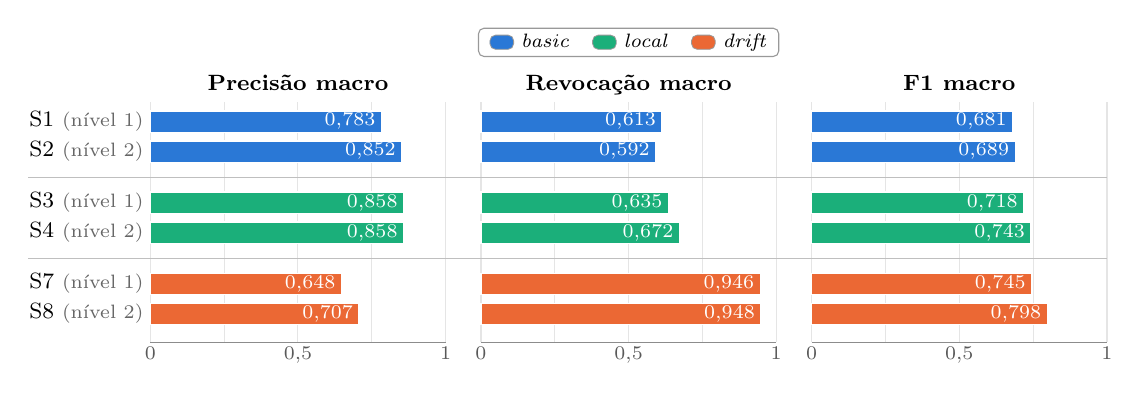
\begin{tikzpicture}[x=1cm, y=1cm, font=\footnotesize]
\def\X{1.75}\def\W{3.75}\def\G{0.45}\def\H{0.27}
\node[anchor=south, draw=black!40, line width=0.4pt, rounded corners=2pt, inner xsep=4pt, inner ysep=2pt, font=\scriptsize]
  at ({\X+1.5*\W+\G},0.42) {\chip{modoBasic}\textit{basic}\hspace{8pt}\chip{modoLocal}\textit{local}\hspace{8pt}\chip{modoDrift}\textit{drift}};
\foreach \k/\tit in {0/Precisão macro, 1/Revocação macro, 2/F1 macro}{
  \pgfmathsetmacro{\x}{\X+\k*(\W+\G)}
  \node[font=\footnotesize\bfseries, anchor=base, inner sep=1pt] at ({\x+\W/2},0.0) {\tit};
  \foreach \t/\lab in {0/0, 0.25/{}, 0.5/{0,5}, 0.75/{}, 1/1}{
    \draw[black!10, line width=0.4pt] ({\x+\W*\t},-0.15) -- ({\x+\W*\t},-3.20);
    \node[anchor=north, inner sep=1.5pt, text=black!65, font=\scriptsize] at ({\x+\W*\t},-3.20) {\lab};
  }
  \draw[black!45, line width=0.4pt] (\x,-3.20) -- ({\x+\W},-3.20);
}
\foreach \s/\n/\c/\y/\p/\r/\f in {
    S1/1/modoBasic/-0.40/0.783/0.613/0.681,
    S2/2/modoBasic/-0.78/0.852/0.592/0.689,
    S3/1/modoLocal/-1.43/0.858/0.635/0.718,
    S4/2/modoLocal/-1.81/0.858/0.672/0.743,
    S7/1/modoDrift/-2.46/0.648/0.946/0.745,
    S8/2/modoDrift/-2.84/0.707/0.948/0.798}{
  \node[anchor=east, inner sep=0pt] at ({\X-0.08},\y) {\s\ {\scriptsize\color{black!60}(nível \n)}};
  \foreach \k/\v in {0/\p, 1/\r, 2/\f}{
    \pgfmathsetmacro{\x}{\X+\k*(\W+\G)}
    \path[fill=\c, draw=white, line width=0.45pt] (\x,{\y+\H/2}) rectangle ({\x+\W*\v},{\y-\H/2});
    \node[anchor=east, inner sep=2pt, text=white, font=\scriptsize] at ({\x+\W*\v},\y)
      {\pgfmathprintnumber[fixed, precision=3, fixed zerofill, use comma]{\v}};
  }
}
\foreach \ys in {-1.105, -2.135}{\draw[black!25, line width=0.4pt] (0.2,\ys) -- ({\X+3*\W+2*\G},\ys);}
\end{tikzpicture}
\caption[Precisão, revocação e F1 macro por sistema]{Precisão, revocação e F1 macro por sistema.}
\label{fig:res-f1-sistemas}
\par\smallskip{\footnotesize Fonte: elaborado pelo autor a partir de \texttt{metricas\_parcial\_sem\_global.csv}.}
\end{figure}

\section{Desempenho por doença}\label{sec:res-por-doenca}

A Figura~\ref{fig:res-f1-doenca} compara o F1 por doença entre os modos \textit{basic} (referência sem uso estruturado do grafo), \textit{local} e \textit{drift} nos dois níveis de comunidade avaliados: S1, S3 e S7, no nível 1 (painel a), e S2, S4 e S8, no nível 2 (painel b). O padrão confirma, com ressalvas, a distinção entre doenças de marcador binário claro e doenças de inferência indireta. Em cirrose hepática e hipertensão portal, doenças que dependem de inferência a partir de múltiplos achados dispersos no texto, o ganho do \textit{drift} sobre o \textit{basic} é o maior nos dois níveis: 18,1 e 19,7 pontos de F1 no nível 1, e 23,1 e 22,1 pontos no nível 2. Em esteatose hepática e hepatite C, cujo texto costuma registrar um exame ou laudo objetivo, o ganho é menor, por efeito-teto (o \textit{basic} já desempenha bem nessas classes): 5,4 e 9,0 pontos no nível 1, e 9,6 e 12,7 no nível 2. A esquistossomose, apesar de também depender de inferência indireta, tem ganho modesto nos dois níveis (5,0 e 8,6 pontos), semelhante ao das doenças de marcador direto.

As duas exceções observadas no nível 1 não se repetem no nível 2. Na hepatite B, o \textit{drift} fica ligeiramente abaixo do \textit{basic} no nível 1 (0,851 contra 0,864), mas o supera no nível 2 (0,927 contra 0,857). Na hemorragia digestiva alta (HDA), o \textit{drift} não supera o \textit{local} no nível 1 (0,457 contra 0,485) e, no nível 2, é o melhor dos três modos, mas com F1 ainda baixo (0,486). Em ambos os níveis, a HDA tem o pior desempenho entre as sete doenças avaliáveis, apesar de o termo literal estar presente na maior parte dos prontuários positivos, o que é consistente com o mecanismo de confusão anatômica investigado e estatisticamente confirmado na Seção~\ref{sec:res-investigacao-erro}. No nível 2, portanto, o \textit{drift} obtém o maior F1 em todas as doenças, e a vantagem continua concentrada nas de evidência indireta.

\begin{figure}[!htbp]
\centering
% Barra proporcional dentro de cada célula, como no painel de acurácia de
% OA-RAG (arXiv:2610.36335); setas de ganho/perda (\gain/\loss) do mesmo artigo.
\resizebox{\textwidth}{!}{%
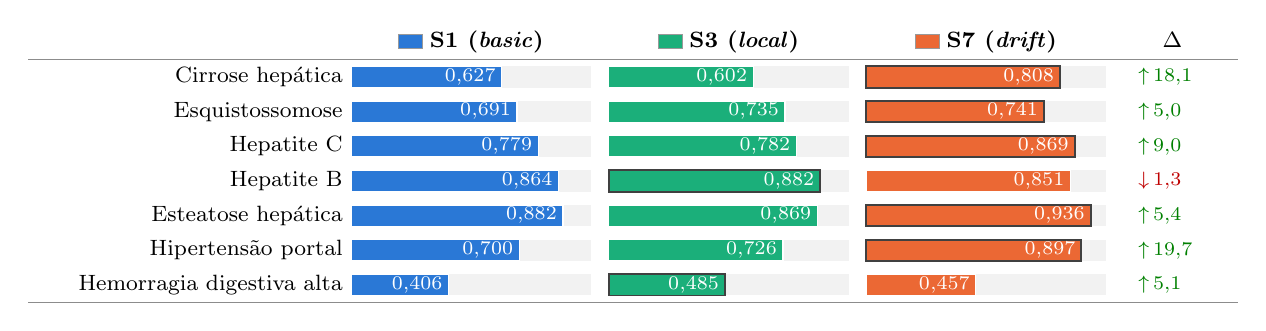
\begin{tikzpicture}[x=1cm, y=1cm, font=\footnotesize]
\def\X{3.95}\def\CW{3.05}\def\GX{0.22}\def\RH{0.44}\def\BH{0.27}
\foreach \k/\tit/\c in {0/{S1 (\textit{basic})}/modoBasic, 1/{S3 (\textit{local})}/modoLocal, 2/{S7 (\textit{drift})}/modoDrift}{
  \node[font=\footnotesize\bfseries, anchor=base, inner sep=1pt] at ({\X+\k*(\CW+\GX)+\CW/2},0.08) {\chip{\c}\tit};
}
\node[font=\footnotesize\bfseries, anchor=base, inner sep=1pt] at ({\X+3*(\CW+\GX)+0.62},0.08) {$\Delta$};
\draw[black!45, line width=0.4pt] (-0.15,-0.08) -- ({\X+3*(\CW+\GX)+1.45},-0.08);
\foreach \i/\nome/\a/\b/\d/\best/\delta in {
    1/Cirrose hepática/0.627/0.602/0.808/2/{\gain{18,1}},
    2/Esquistossomose/0.691/0.735/0.741/2/{\gain{5,0}},
    3/Hepatite C/0.779/0.782/0.869/2/{\gain{9,0}},
    4/Hepatite B/0.864/0.882/0.851/1/{\loss{1,3}},
    5/Esteatose hepática/0.882/0.869/0.936/2/{\gain{5,4}},
    6/Hipertensão portal/0.700/0.726/0.897/2/{\gain{19,7}},
    7/{Hemorragia digestiva alta}/0.406/0.485/0.457/1/{\gain{5,1}}}{
  \pgfmathsetmacro{\y}{-0.08-\i*\RH+\RH/2}
  \node[anchor=east, inner sep=0pt] at ({\X-0.10},\y) {\nome};
  \foreach \k/\v/\c in {0/\a/modoBasic, 1/\b/modoLocal, 2/\d/modoDrift}{
    \pgfmathsetmacro{\x}{\X+\k*(\CW+\GX)}
    \fill[black!5] (\x,{\y+\BH/2}) rectangle ({\x+\CW},{\y-\BH/2});
    \path[fill=\c, draw=white, line width=0.45pt] (\x,{\y+\BH/2}) rectangle ({\x+\CW*\v},{\y-\BH/2});
    \ifnum\k=\best\draw[black!75, line width=0.7pt] (\x,{\y+\BH/2}) rectangle ({\x+\CW*\v},{\y-\BH/2});\fi
    \node[anchor=east, inner sep=2pt, text=white, font=\scriptsize] at ({\x+\CW*\v},\y)
      {\ifnum\k=\best\bfseries\fi\pgfmathprintnumber[fixed, precision=3, fixed zerofill, use comma]{\v}};
  }
  \node[anchor=west, inner sep=0pt, font=\scriptsize] at ({\X+3*(\CW+\GX)+0.10},\y) {\delta};
}
\draw[black!45, line width=0.4pt] (-0.15,{-0.08-7*\RH}) -- ({\X+3*(\CW+\GX)+1.45},{-0.08-7*\RH});
\end{tikzpicture}}\\[2pt]
{\footnotesize (a) Nível 1}
\\[8pt]
\resizebox{\textwidth}{!}{%
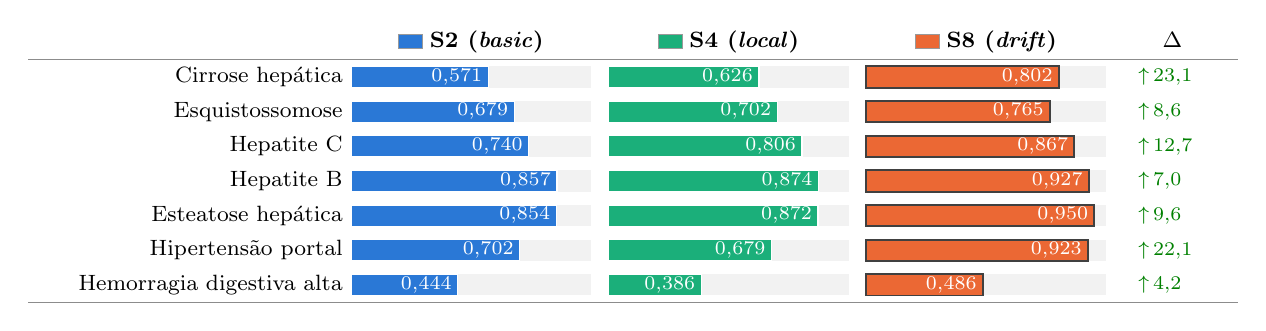
\begin{tikzpicture}[x=1cm, y=1cm, font=\footnotesize]
\def\X{3.95}\def\CW{3.05}\def\GX{0.22}\def\RH{0.44}\def\BH{0.27}
\foreach \k/\tit/\c in {0/{S2 (\textit{basic})}/modoBasic, 1/{S4 (\textit{local})}/modoLocal, 2/{S8 (\textit{drift})}/modoDrift}{
  \node[font=\footnotesize\bfseries, anchor=base, inner sep=1pt] at ({\X+\k*(\CW+\GX)+\CW/2},0.08) {\chip{\c}\tit};
}
\node[font=\footnotesize\bfseries, anchor=base, inner sep=1pt] at ({\X+3*(\CW+\GX)+0.62},0.08) {$\Delta$};
\draw[black!45, line width=0.4pt] (-0.15,-0.08) -- ({\X+3*(\CW+\GX)+1.45},-0.08);
\foreach \i/\nome/\a/\b/\d/\best/\delta in {
    1/Cirrose hepática/0.571/0.626/0.802/2/{\gain{23,1}},
    2/Esquistossomose/0.679/0.702/0.765/2/{\gain{8,6}},
    3/Hepatite C/0.740/0.806/0.867/2/{\gain{12,7}},
    4/Hepatite B/0.857/0.874/0.927/2/{\gain{7,0}},
    5/Esteatose hepática/0.854/0.872/0.950/2/{\gain{9,6}},
    6/Hipertensão portal/0.702/0.679/0.923/2/{\gain{22,1}},
    7/{Hemorragia digestiva alta}/0.444/0.386/0.486/2/{\gain{4,2}}}{
  \pgfmathsetmacro{\y}{-0.08-\i*\RH+\RH/2}
  \node[anchor=east, inner sep=0pt] at ({\X-0.10},\y) {\nome};
  \foreach \k/\v/\c in {0/\a/modoBasic, 1/\b/modoLocal, 2/\d/modoDrift}{
    \pgfmathsetmacro{\x}{\X+\k*(\CW+\GX)}
    \fill[black!5] (\x,{\y+\BH/2}) rectangle ({\x+\CW},{\y-\BH/2});
    \path[fill=\c, draw=white, line width=0.45pt] (\x,{\y+\BH/2}) rectangle ({\x+\CW*\v},{\y-\BH/2});
    \ifnum\k=\best\draw[black!75, line width=0.7pt] (\x,{\y+\BH/2}) rectangle ({\x+\CW*\v},{\y-\BH/2});\fi
    \node[anchor=east, inner sep=2pt, text=white, font=\scriptsize] at ({\x+\CW*\v},\y)
      {\ifnum\k=\best\bfseries\fi\pgfmathprintnumber[fixed, precision=3, fixed zerofill, use comma]{\v}};
  }
  \node[anchor=west, inner sep=0pt, font=\scriptsize] at ({\X+3*(\CW+\GX)+0.10},\y) {\delta};
}
\draw[black!45, line width=0.4pt] (-0.15,{-0.08-7*\RH}) -- ({\X+3*(\CW+\GX)+1.45},{-0.08-7*\RH});
\end{tikzpicture}}\\[2pt]
{\footnotesize (b) Nível 2}

\caption[F1 por doença, por modo de busca e nível de comunidade]{F1 por doença nos níveis de comunidade 1 (a) e 2 (b); $\Delta$ é a diferença, em pontos de F1, entre o \textit{drift} e o \textit{basic} do mesmo nível.}
\label{fig:res-f1-doenca}
\par\smallskip{\footnotesize Fonte: elaborado pelo autor a partir de \texttt{metricas\_parcial\_sem\_global.csv}.}
\end{figure}

As matrizes de confusão por doença (Figuras~\ref{fig:res-confusao-s7} e~\ref{fig:res-confusao-s8}) detalham essa distribuição para o modo \textit{drift}, permitindo identificar em qual direção -- falso positivo ou falso negativo -- se concentra o erro de cada classe.

\begin{figure}[!htbp]
\centering
% Gerado por experiments/grid_search/gera_matrizes_confusao_tikz.py -- não editar à mão
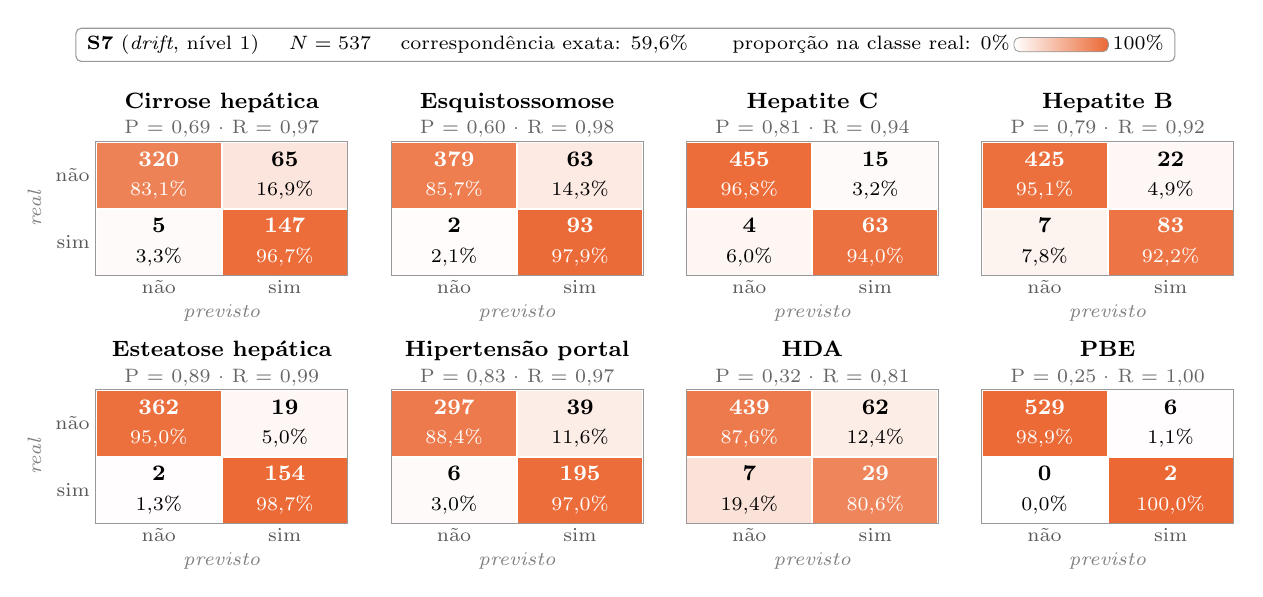
\begin{tikzpicture}[x=1cm, y=1cm, font=\footnotesize]
\node[anchor=north, draw=black!40, line width=0.4pt, rounded corners=2pt, inner xsep=4pt, inner ysep=2.5pt, font=\scriptsize] at (7.725,1.45) {\textbf{S7} (\textit{drift}, nível 1) \quad $N=537$ \quad correspondência exata: 59,6\%\qquad proporção na classe real: 0\%\,\tikz[baseline=-0.6ex]{\shade[left color=white, right color=modoDrift, draw=black!40, line width=0.3pt] (0,-0.09) rectangle (1.2,0.09);}\,100\%};
\node[anchor=base, font=\footnotesize\bfseries, inner sep=0pt] at (2.600,0.420) {Cirrose hepática};
\node[anchor=base, font=\scriptsize, text=black!60, inner sep=0pt] at (2.600,0.100) {P = 0,69 \textperiodcentered\ R = 0,97};
\path[fill=modoDrift!83!white, draw=white, line width=0.8pt] (1.000,0.000) rectangle (2.600,-0.850);
\node[align=center, inner sep=0pt, text=white, font=\footnotesize] at (1.800,-0.425) {\textbf{320}\\[1pt]{\scriptsize 83,1\%}};
\path[fill=modoDrift!17!white, draw=white, line width=0.8pt] (2.600,0.000) rectangle (4.200,-0.850);
\node[align=center, inner sep=0pt, text=black, font=\footnotesize] at (3.400,-0.425) {\textbf{65}\\[1pt]{\scriptsize 16,9\%}};
\path[fill=modoDrift!3!white, draw=white, line width=0.8pt] (1.000,-0.850) rectangle (2.600,-1.700);
\node[align=center, inner sep=0pt, text=black, font=\footnotesize] at (1.800,-1.275) {\textbf{5}\\[1pt]{\scriptsize 3,3\%}};
\path[fill=modoDrift!97!white, draw=white, line width=0.8pt] (2.600,-0.850) rectangle (4.200,-1.700);
\node[align=center, inner sep=0pt, text=white, font=\footnotesize] at (3.400,-1.275) {\textbf{147}\\[1pt]{\scriptsize 96,7\%}};
\draw[black!40, line width=0.4pt] (1.000,0.000) rectangle (4.200,-1.700);
\node[anchor=north, font=\scriptsize, text=black!65, inner sep=1.5pt] at (1.800,-1.700) {não};
\node[anchor=north, font=\scriptsize, text=black!65, inner sep=1.5pt] at (3.400,-1.700) {sim};
\node[anchor=north, font=\scriptsize\itshape, text=black!50, inner sep=0pt] at (2.600,-2.060) {previsto};
\node[anchor=east, font=\scriptsize, text=black!65, inner sep=2pt] at (1.000,-0.425) {não};
\node[anchor=east, font=\scriptsize, text=black!65, inner sep=2pt] at (1.000,-1.275) {sim};
\node[rotate=90, font=\scriptsize\itshape, text=black!50, inner sep=0pt] at (0.220,-0.850) {real};
\node[anchor=base, font=\footnotesize\bfseries, inner sep=0pt] at (6.350,0.420) {Esquistossomose};
\node[anchor=base, font=\scriptsize, text=black!60, inner sep=0pt] at (6.350,0.100) {P = 0,60 \textperiodcentered\ R = 0,98};
\path[fill=modoDrift!86!white, draw=white, line width=0.8pt] (4.750,0.000) rectangle (6.350,-0.850);
\node[align=center, inner sep=0pt, text=white, font=\footnotesize] at (5.550,-0.425) {\textbf{379}\\[1pt]{\scriptsize 85,7\%}};
\path[fill=modoDrift!14!white, draw=white, line width=0.8pt] (6.350,0.000) rectangle (7.950,-0.850);
\node[align=center, inner sep=0pt, text=black, font=\footnotesize] at (7.150,-0.425) {\textbf{63}\\[1pt]{\scriptsize 14,3\%}};
\path[fill=modoDrift!2!white, draw=white, line width=0.8pt] (4.750,-0.850) rectangle (6.350,-1.700);
\node[align=center, inner sep=0pt, text=black, font=\footnotesize] at (5.550,-1.275) {\textbf{2}\\[1pt]{\scriptsize 2,1\%}};
\path[fill=modoDrift!98!white, draw=white, line width=0.8pt] (6.350,-0.850) rectangle (7.950,-1.700);
\node[align=center, inner sep=0pt, text=white, font=\footnotesize] at (7.150,-1.275) {\textbf{93}\\[1pt]{\scriptsize 97,9\%}};
\draw[black!40, line width=0.4pt] (4.750,0.000) rectangle (7.950,-1.700);
\node[anchor=north, font=\scriptsize, text=black!65, inner sep=1.5pt] at (5.550,-1.700) {não};
\node[anchor=north, font=\scriptsize, text=black!65, inner sep=1.5pt] at (7.150,-1.700) {sim};
\node[anchor=north, font=\scriptsize\itshape, text=black!50, inner sep=0pt] at (6.350,-2.060) {previsto};
\node[anchor=base, font=\footnotesize\bfseries, inner sep=0pt] at (10.100,0.420) {Hepatite C};
\node[anchor=base, font=\scriptsize, text=black!60, inner sep=0pt] at (10.100,0.100) {P = 0,81 \textperiodcentered\ R = 0,94};
\path[fill=modoDrift!97!white, draw=white, line width=0.8pt] (8.500,0.000) rectangle (10.100,-0.850);
\node[align=center, inner sep=0pt, text=white, font=\footnotesize] at (9.300,-0.425) {\textbf{455}\\[1pt]{\scriptsize 96,8\%}};
\path[fill=modoDrift!3!white, draw=white, line width=0.8pt] (10.100,0.000) rectangle (11.700,-0.850);
\node[align=center, inner sep=0pt, text=black, font=\footnotesize] at (10.900,-0.425) {\textbf{15}\\[1pt]{\scriptsize 3,2\%}};
\path[fill=modoDrift!6!white, draw=white, line width=0.8pt] (8.500,-0.850) rectangle (10.100,-1.700);
\node[align=center, inner sep=0pt, text=black, font=\footnotesize] at (9.300,-1.275) {\textbf{4}\\[1pt]{\scriptsize 6,0\%}};
\path[fill=modoDrift!94!white, draw=white, line width=0.8pt] (10.100,-0.850) rectangle (11.700,-1.700);
\node[align=center, inner sep=0pt, text=white, font=\footnotesize] at (10.900,-1.275) {\textbf{63}\\[1pt]{\scriptsize 94,0\%}};
\draw[black!40, line width=0.4pt] (8.500,0.000) rectangle (11.700,-1.700);
\node[anchor=north, font=\scriptsize, text=black!65, inner sep=1.5pt] at (9.300,-1.700) {não};
\node[anchor=north, font=\scriptsize, text=black!65, inner sep=1.5pt] at (10.900,-1.700) {sim};
\node[anchor=north, font=\scriptsize\itshape, text=black!50, inner sep=0pt] at (10.100,-2.060) {previsto};
\node[anchor=base, font=\footnotesize\bfseries, inner sep=0pt] at (13.850,0.420) {Hepatite B};
\node[anchor=base, font=\scriptsize, text=black!60, inner sep=0pt] at (13.850,0.100) {P = 0,79 \textperiodcentered\ R = 0,92};
\path[fill=modoDrift!95!white, draw=white, line width=0.8pt] (12.250,0.000) rectangle (13.850,-0.850);
\node[align=center, inner sep=0pt, text=white, font=\footnotesize] at (13.050,-0.425) {\textbf{425}\\[1pt]{\scriptsize 95,1\%}};
\path[fill=modoDrift!5!white, draw=white, line width=0.8pt] (13.850,0.000) rectangle (15.450,-0.850);
\node[align=center, inner sep=0pt, text=black, font=\footnotesize] at (14.650,-0.425) {\textbf{22}\\[1pt]{\scriptsize 4,9\%}};
\path[fill=modoDrift!8!white, draw=white, line width=0.8pt] (12.250,-0.850) rectangle (13.850,-1.700);
\node[align=center, inner sep=0pt, text=black, font=\footnotesize] at (13.050,-1.275) {\textbf{7}\\[1pt]{\scriptsize 7,8\%}};
\path[fill=modoDrift!92!white, draw=white, line width=0.8pt] (13.850,-0.850) rectangle (15.450,-1.700);
\node[align=center, inner sep=0pt, text=white, font=\footnotesize] at (14.650,-1.275) {\textbf{83}\\[1pt]{\scriptsize 92,2\%}};
\draw[black!40, line width=0.4pt] (12.250,0.000) rectangle (15.450,-1.700);
\node[anchor=north, font=\scriptsize, text=black!65, inner sep=1.5pt] at (13.050,-1.700) {não};
\node[anchor=north, font=\scriptsize, text=black!65, inner sep=1.5pt] at (14.650,-1.700) {sim};
\node[anchor=north, font=\scriptsize\itshape, text=black!50, inner sep=0pt] at (13.850,-2.060) {previsto};
\node[anchor=base, font=\footnotesize\bfseries, inner sep=0pt] at (2.600,-2.730) {Esteatose hepática};
\node[anchor=base, font=\scriptsize, text=black!60, inner sep=0pt] at (2.600,-3.050) {P = 0,89 \textperiodcentered\ R = 0,99};
\path[fill=modoDrift!95!white, draw=white, line width=0.8pt] (1.000,-3.150) rectangle (2.600,-4.000);
\node[align=center, inner sep=0pt, text=white, font=\footnotesize] at (1.800,-3.575) {\textbf{362}\\[1pt]{\scriptsize 95,0\%}};
\path[fill=modoDrift!5!white, draw=white, line width=0.8pt] (2.600,-3.150) rectangle (4.200,-4.000);
\node[align=center, inner sep=0pt, text=black, font=\footnotesize] at (3.400,-3.575) {\textbf{19}\\[1pt]{\scriptsize 5,0\%}};
\path[fill=modoDrift!1!white, draw=white, line width=0.8pt] (1.000,-4.000) rectangle (2.600,-4.850);
\node[align=center, inner sep=0pt, text=black, font=\footnotesize] at (1.800,-4.425) {\textbf{2}\\[1pt]{\scriptsize 1,3\%}};
\path[fill=modoDrift!99!white, draw=white, line width=0.8pt] (2.600,-4.000) rectangle (4.200,-4.850);
\node[align=center, inner sep=0pt, text=white, font=\footnotesize] at (3.400,-4.425) {\textbf{154}\\[1pt]{\scriptsize 98,7\%}};
\draw[black!40, line width=0.4pt] (1.000,-3.150) rectangle (4.200,-4.850);
\node[anchor=north, font=\scriptsize, text=black!65, inner sep=1.5pt] at (1.800,-4.850) {não};
\node[anchor=north, font=\scriptsize, text=black!65, inner sep=1.5pt] at (3.400,-4.850) {sim};
\node[anchor=north, font=\scriptsize\itshape, text=black!50, inner sep=0pt] at (2.600,-5.210) {previsto};
\node[anchor=east, font=\scriptsize, text=black!65, inner sep=2pt] at (1.000,-3.575) {não};
\node[anchor=east, font=\scriptsize, text=black!65, inner sep=2pt] at (1.000,-4.425) {sim};
\node[rotate=90, font=\scriptsize\itshape, text=black!50, inner sep=0pt] at (0.220,-4.000) {real};
\node[anchor=base, font=\footnotesize\bfseries, inner sep=0pt] at (6.350,-2.730) {Hipertensão portal};
\node[anchor=base, font=\scriptsize, text=black!60, inner sep=0pt] at (6.350,-3.050) {P = 0,83 \textperiodcentered\ R = 0,97};
\path[fill=modoDrift!88!white, draw=white, line width=0.8pt] (4.750,-3.150) rectangle (6.350,-4.000);
\node[align=center, inner sep=0pt, text=white, font=\footnotesize] at (5.550,-3.575) {\textbf{297}\\[1pt]{\scriptsize 88,4\%}};
\path[fill=modoDrift!12!white, draw=white, line width=0.8pt] (6.350,-3.150) rectangle (7.950,-4.000);
\node[align=center, inner sep=0pt, text=black, font=\footnotesize] at (7.150,-3.575) {\textbf{39}\\[1pt]{\scriptsize 11,6\%}};
\path[fill=modoDrift!3!white, draw=white, line width=0.8pt] (4.750,-4.000) rectangle (6.350,-4.850);
\node[align=center, inner sep=0pt, text=black, font=\footnotesize] at (5.550,-4.425) {\textbf{6}\\[1pt]{\scriptsize 3,0\%}};
\path[fill=modoDrift!97!white, draw=white, line width=0.8pt] (6.350,-4.000) rectangle (7.950,-4.850);
\node[align=center, inner sep=0pt, text=white, font=\footnotesize] at (7.150,-4.425) {\textbf{195}\\[1pt]{\scriptsize 97,0\%}};
\draw[black!40, line width=0.4pt] (4.750,-3.150) rectangle (7.950,-4.850);
\node[anchor=north, font=\scriptsize, text=black!65, inner sep=1.5pt] at (5.550,-4.850) {não};
\node[anchor=north, font=\scriptsize, text=black!65, inner sep=1.5pt] at (7.150,-4.850) {sim};
\node[anchor=north, font=\scriptsize\itshape, text=black!50, inner sep=0pt] at (6.350,-5.210) {previsto};
\node[anchor=base, font=\footnotesize\bfseries, inner sep=0pt] at (10.100,-2.730) {HDA};
\node[anchor=base, font=\scriptsize, text=black!60, inner sep=0pt] at (10.100,-3.050) {P = 0,32 \textperiodcentered\ R = 0,81};
\path[fill=modoDrift!88!white, draw=white, line width=0.8pt] (8.500,-3.150) rectangle (10.100,-4.000);
\node[align=center, inner sep=0pt, text=white, font=\footnotesize] at (9.300,-3.575) {\textbf{439}\\[1pt]{\scriptsize 87,6\%}};
\path[fill=modoDrift!12!white, draw=white, line width=0.8pt] (10.100,-3.150) rectangle (11.700,-4.000);
\node[align=center, inner sep=0pt, text=black, font=\footnotesize] at (10.900,-3.575) {\textbf{62}\\[1pt]{\scriptsize 12,4\%}};
\path[fill=modoDrift!19!white, draw=white, line width=0.8pt] (8.500,-4.000) rectangle (10.100,-4.850);
\node[align=center, inner sep=0pt, text=black, font=\footnotesize] at (9.300,-4.425) {\textbf{7}\\[1pt]{\scriptsize 19,4\%}};
\path[fill=modoDrift!81!white, draw=white, line width=0.8pt] (10.100,-4.000) rectangle (11.700,-4.850);
\node[align=center, inner sep=0pt, text=white, font=\footnotesize] at (10.900,-4.425) {\textbf{29}\\[1pt]{\scriptsize 80,6\%}};
\draw[black!40, line width=0.4pt] (8.500,-3.150) rectangle (11.700,-4.850);
\node[anchor=north, font=\scriptsize, text=black!65, inner sep=1.5pt] at (9.300,-4.850) {não};
\node[anchor=north, font=\scriptsize, text=black!65, inner sep=1.5pt] at (10.900,-4.850) {sim};
\node[anchor=north, font=\scriptsize\itshape, text=black!50, inner sep=0pt] at (10.100,-5.210) {previsto};
\node[anchor=base, font=\footnotesize\bfseries, inner sep=0pt] at (13.850,-2.730) {PBE};
\node[anchor=base, font=\scriptsize, text=black!60, inner sep=0pt] at (13.850,-3.050) {P = 0,25 \textperiodcentered\ R = 1,00};
\path[fill=modoDrift!99!white, draw=white, line width=0.8pt] (12.250,-3.150) rectangle (13.850,-4.000);
\node[align=center, inner sep=0pt, text=white, font=\footnotesize] at (13.050,-3.575) {\textbf{529}\\[1pt]{\scriptsize 98,9\%}};
\path[fill=modoDrift!1!white, draw=white, line width=0.8pt] (13.850,-3.150) rectangle (15.450,-4.000);
\node[align=center, inner sep=0pt, text=black, font=\footnotesize] at (14.650,-3.575) {\textbf{6}\\[1pt]{\scriptsize 1,1\%}};
\path[fill=modoDrift!0!white, draw=white, line width=0.8pt] (12.250,-4.000) rectangle (13.850,-4.850);
\node[align=center, inner sep=0pt, text=black, font=\footnotesize] at (13.050,-4.425) {\textbf{0}\\[1pt]{\scriptsize 0,0\%}};
\path[fill=modoDrift!100!white, draw=white, line width=0.8pt] (13.850,-4.000) rectangle (15.450,-4.850);
\node[align=center, inner sep=0pt, text=white, font=\footnotesize] at (14.650,-4.425) {\textbf{2}\\[1pt]{\scriptsize 100,0\%}};
\draw[black!40, line width=0.4pt] (12.250,-3.150) rectangle (15.450,-4.850);
\node[anchor=north, font=\scriptsize, text=black!65, inner sep=1.5pt] at (13.050,-4.850) {não};
\node[anchor=north, font=\scriptsize, text=black!65, inner sep=1.5pt] at (14.650,-4.850) {sim};
\node[anchor=north, font=\scriptsize\itshape, text=black!50, inner sep=0pt] at (13.850,-5.210) {previsto};
\end{tikzpicture}

\caption[Matrizes de confusão por doença, sistema S7]{Matrizes de confusão por doença, sistema S7 (\textit{drift}, nível 1), com contagem e proporção na classe real.}
\label{fig:res-confusao-s7}
\par\smallskip{\footnotesize Fonte: elaborado pelo autor.}
\end{figure}

\begin{figure}[!htbp]
\centering
% Gerado por experiments/grid_search/gera_matrizes_confusao_tikz.py -- não editar à mão
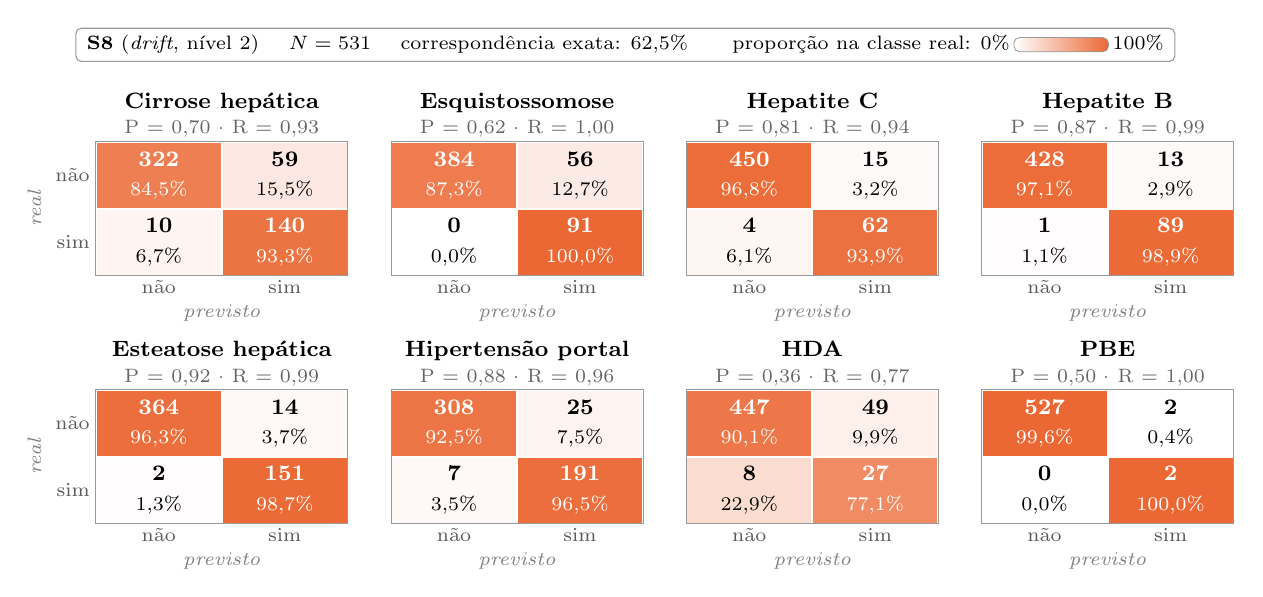
\begin{tikzpicture}[x=1cm, y=1cm, font=\footnotesize]
\node[anchor=north, draw=black!40, line width=0.4pt, rounded corners=2pt, inner xsep=4pt, inner ysep=2.5pt, font=\scriptsize] at (7.725,1.45) {\textbf{S8} (\textit{drift}, nível 2) \quad $N=531$ \quad correspondência exata: 62,5\%\qquad proporção na classe real: 0\%\,\tikz[baseline=-0.6ex]{\shade[left color=white, right color=modoDrift, draw=black!40, line width=0.3pt] (0,-0.09) rectangle (1.2,0.09);}\,100\%};
\node[anchor=base, font=\footnotesize\bfseries, inner sep=0pt] at (2.600,0.420) {Cirrose hepática};
\node[anchor=base, font=\scriptsize, text=black!60, inner sep=0pt] at (2.600,0.100) {P = 0,70 \textperiodcentered\ R = 0,93};
\path[fill=modoDrift!85!white, draw=white, line width=0.8pt] (1.000,0.000) rectangle (2.600,-0.850);
\node[align=center, inner sep=0pt, text=white, font=\footnotesize] at (1.800,-0.425) {\textbf{322}\\[1pt]{\scriptsize 84,5\%}};
\path[fill=modoDrift!15!white, draw=white, line width=0.8pt] (2.600,0.000) rectangle (4.200,-0.850);
\node[align=center, inner sep=0pt, text=black, font=\footnotesize] at (3.400,-0.425) {\textbf{59}\\[1pt]{\scriptsize 15,5\%}};
\path[fill=modoDrift!7!white, draw=white, line width=0.8pt] (1.000,-0.850) rectangle (2.600,-1.700);
\node[align=center, inner sep=0pt, text=black, font=\footnotesize] at (1.800,-1.275) {\textbf{10}\\[1pt]{\scriptsize 6,7\%}};
\path[fill=modoDrift!93!white, draw=white, line width=0.8pt] (2.600,-0.850) rectangle (4.200,-1.700);
\node[align=center, inner sep=0pt, text=white, font=\footnotesize] at (3.400,-1.275) {\textbf{140}\\[1pt]{\scriptsize 93,3\%}};
\draw[black!40, line width=0.4pt] (1.000,0.000) rectangle (4.200,-1.700);
\node[anchor=north, font=\scriptsize, text=black!65, inner sep=1.5pt] at (1.800,-1.700) {não};
\node[anchor=north, font=\scriptsize, text=black!65, inner sep=1.5pt] at (3.400,-1.700) {sim};
\node[anchor=north, font=\scriptsize\itshape, text=black!50, inner sep=0pt] at (2.600,-2.060) {previsto};
\node[anchor=east, font=\scriptsize, text=black!65, inner sep=2pt] at (1.000,-0.425) {não};
\node[anchor=east, font=\scriptsize, text=black!65, inner sep=2pt] at (1.000,-1.275) {sim};
\node[rotate=90, font=\scriptsize\itshape, text=black!50, inner sep=0pt] at (0.220,-0.850) {real};
\node[anchor=base, font=\footnotesize\bfseries, inner sep=0pt] at (6.350,0.420) {Esquistossomose};
\node[anchor=base, font=\scriptsize, text=black!60, inner sep=0pt] at (6.350,0.100) {P = 0,62 \textperiodcentered\ R = 1,00};
\path[fill=modoDrift!87!white, draw=white, line width=0.8pt] (4.750,0.000) rectangle (6.350,-0.850);
\node[align=center, inner sep=0pt, text=white, font=\footnotesize] at (5.550,-0.425) {\textbf{384}\\[1pt]{\scriptsize 87,3\%}};
\path[fill=modoDrift!13!white, draw=white, line width=0.8pt] (6.350,0.000) rectangle (7.950,-0.850);
\node[align=center, inner sep=0pt, text=black, font=\footnotesize] at (7.150,-0.425) {\textbf{56}\\[1pt]{\scriptsize 12,7\%}};
\path[fill=modoDrift!0!white, draw=white, line width=0.8pt] (4.750,-0.850) rectangle (6.350,-1.700);
\node[align=center, inner sep=0pt, text=black, font=\footnotesize] at (5.550,-1.275) {\textbf{0}\\[1pt]{\scriptsize 0,0\%}};
\path[fill=modoDrift!100!white, draw=white, line width=0.8pt] (6.350,-0.850) rectangle (7.950,-1.700);
\node[align=center, inner sep=0pt, text=white, font=\footnotesize] at (7.150,-1.275) {\textbf{91}\\[1pt]{\scriptsize 100,0\%}};
\draw[black!40, line width=0.4pt] (4.750,0.000) rectangle (7.950,-1.700);
\node[anchor=north, font=\scriptsize, text=black!65, inner sep=1.5pt] at (5.550,-1.700) {não};
\node[anchor=north, font=\scriptsize, text=black!65, inner sep=1.5pt] at (7.150,-1.700) {sim};
\node[anchor=north, font=\scriptsize\itshape, text=black!50, inner sep=0pt] at (6.350,-2.060) {previsto};
\node[anchor=base, font=\footnotesize\bfseries, inner sep=0pt] at (10.100,0.420) {Hepatite C};
\node[anchor=base, font=\scriptsize, text=black!60, inner sep=0pt] at (10.100,0.100) {P = 0,81 \textperiodcentered\ R = 0,94};
\path[fill=modoDrift!97!white, draw=white, line width=0.8pt] (8.500,0.000) rectangle (10.100,-0.850);
\node[align=center, inner sep=0pt, text=white, font=\footnotesize] at (9.300,-0.425) {\textbf{450}\\[1pt]{\scriptsize 96,8\%}};
\path[fill=modoDrift!3!white, draw=white, line width=0.8pt] (10.100,0.000) rectangle (11.700,-0.850);
\node[align=center, inner sep=0pt, text=black, font=\footnotesize] at (10.900,-0.425) {\textbf{15}\\[1pt]{\scriptsize 3,2\%}};
\path[fill=modoDrift!6!white, draw=white, line width=0.8pt] (8.500,-0.850) rectangle (10.100,-1.700);
\node[align=center, inner sep=0pt, text=black, font=\footnotesize] at (9.300,-1.275) {\textbf{4}\\[1pt]{\scriptsize 6,1\%}};
\path[fill=modoDrift!94!white, draw=white, line width=0.8pt] (10.100,-0.850) rectangle (11.700,-1.700);
\node[align=center, inner sep=0pt, text=white, font=\footnotesize] at (10.900,-1.275) {\textbf{62}\\[1pt]{\scriptsize 93,9\%}};
\draw[black!40, line width=0.4pt] (8.500,0.000) rectangle (11.700,-1.700);
\node[anchor=north, font=\scriptsize, text=black!65, inner sep=1.5pt] at (9.300,-1.700) {não};
\node[anchor=north, font=\scriptsize, text=black!65, inner sep=1.5pt] at (10.900,-1.700) {sim};
\node[anchor=north, font=\scriptsize\itshape, text=black!50, inner sep=0pt] at (10.100,-2.060) {previsto};
\node[anchor=base, font=\footnotesize\bfseries, inner sep=0pt] at (13.850,0.420) {Hepatite B};
\node[anchor=base, font=\scriptsize, text=black!60, inner sep=0pt] at (13.850,0.100) {P = 0,87 \textperiodcentered\ R = 0,99};
\path[fill=modoDrift!97!white, draw=white, line width=0.8pt] (12.250,0.000) rectangle (13.850,-0.850);
\node[align=center, inner sep=0pt, text=white, font=\footnotesize] at (13.050,-0.425) {\textbf{428}\\[1pt]{\scriptsize 97,1\%}};
\path[fill=modoDrift!3!white, draw=white, line width=0.8pt] (13.850,0.000) rectangle (15.450,-0.850);
\node[align=center, inner sep=0pt, text=black, font=\footnotesize] at (14.650,-0.425) {\textbf{13}\\[1pt]{\scriptsize 2,9\%}};
\path[fill=modoDrift!1!white, draw=white, line width=0.8pt] (12.250,-0.850) rectangle (13.850,-1.700);
\node[align=center, inner sep=0pt, text=black, font=\footnotesize] at (13.050,-1.275) {\textbf{1}\\[1pt]{\scriptsize 1,1\%}};
\path[fill=modoDrift!99!white, draw=white, line width=0.8pt] (13.850,-0.850) rectangle (15.450,-1.700);
\node[align=center, inner sep=0pt, text=white, font=\footnotesize] at (14.650,-1.275) {\textbf{89}\\[1pt]{\scriptsize 98,9\%}};
\draw[black!40, line width=0.4pt] (12.250,0.000) rectangle (15.450,-1.700);
\node[anchor=north, font=\scriptsize, text=black!65, inner sep=1.5pt] at (13.050,-1.700) {não};
\node[anchor=north, font=\scriptsize, text=black!65, inner sep=1.5pt] at (14.650,-1.700) {sim};
\node[anchor=north, font=\scriptsize\itshape, text=black!50, inner sep=0pt] at (13.850,-2.060) {previsto};
\node[anchor=base, font=\footnotesize\bfseries, inner sep=0pt] at (2.600,-2.730) {Esteatose hepática};
\node[anchor=base, font=\scriptsize, text=black!60, inner sep=0pt] at (2.600,-3.050) {P = 0,92 \textperiodcentered\ R = 0,99};
\path[fill=modoDrift!96!white, draw=white, line width=0.8pt] (1.000,-3.150) rectangle (2.600,-4.000);
\node[align=center, inner sep=0pt, text=white, font=\footnotesize] at (1.800,-3.575) {\textbf{364}\\[1pt]{\scriptsize 96,3\%}};
\path[fill=modoDrift!4!white, draw=white, line width=0.8pt] (2.600,-3.150) rectangle (4.200,-4.000);
\node[align=center, inner sep=0pt, text=black, font=\footnotesize] at (3.400,-3.575) {\textbf{14}\\[1pt]{\scriptsize 3,7\%}};
\path[fill=modoDrift!1!white, draw=white, line width=0.8pt] (1.000,-4.000) rectangle (2.600,-4.850);
\node[align=center, inner sep=0pt, text=black, font=\footnotesize] at (1.800,-4.425) {\textbf{2}\\[1pt]{\scriptsize 1,3\%}};
\path[fill=modoDrift!99!white, draw=white, line width=0.8pt] (2.600,-4.000) rectangle (4.200,-4.850);
\node[align=center, inner sep=0pt, text=white, font=\footnotesize] at (3.400,-4.425) {\textbf{151}\\[1pt]{\scriptsize 98,7\%}};
\draw[black!40, line width=0.4pt] (1.000,-3.150) rectangle (4.200,-4.850);
\node[anchor=north, font=\scriptsize, text=black!65, inner sep=1.5pt] at (1.800,-4.850) {não};
\node[anchor=north, font=\scriptsize, text=black!65, inner sep=1.5pt] at (3.400,-4.850) {sim};
\node[anchor=north, font=\scriptsize\itshape, text=black!50, inner sep=0pt] at (2.600,-5.210) {previsto};
\node[anchor=east, font=\scriptsize, text=black!65, inner sep=2pt] at (1.000,-3.575) {não};
\node[anchor=east, font=\scriptsize, text=black!65, inner sep=2pt] at (1.000,-4.425) {sim};
\node[rotate=90, font=\scriptsize\itshape, text=black!50, inner sep=0pt] at (0.220,-4.000) {real};
\node[anchor=base, font=\footnotesize\bfseries, inner sep=0pt] at (6.350,-2.730) {Hipertensão portal};
\node[anchor=base, font=\scriptsize, text=black!60, inner sep=0pt] at (6.350,-3.050) {P = 0,88 \textperiodcentered\ R = 0,96};
\path[fill=modoDrift!92!white, draw=white, line width=0.8pt] (4.750,-3.150) rectangle (6.350,-4.000);
\node[align=center, inner sep=0pt, text=white, font=\footnotesize] at (5.550,-3.575) {\textbf{308}\\[1pt]{\scriptsize 92,5\%}};
\path[fill=modoDrift!8!white, draw=white, line width=0.8pt] (6.350,-3.150) rectangle (7.950,-4.000);
\node[align=center, inner sep=0pt, text=black, font=\footnotesize] at (7.150,-3.575) {\textbf{25}\\[1pt]{\scriptsize 7,5\%}};
\path[fill=modoDrift!4!white, draw=white, line width=0.8pt] (4.750,-4.000) rectangle (6.350,-4.850);
\node[align=center, inner sep=0pt, text=black, font=\footnotesize] at (5.550,-4.425) {\textbf{7}\\[1pt]{\scriptsize 3,5\%}};
\path[fill=modoDrift!96!white, draw=white, line width=0.8pt] (6.350,-4.000) rectangle (7.950,-4.850);
\node[align=center, inner sep=0pt, text=white, font=\footnotesize] at (7.150,-4.425) {\textbf{191}\\[1pt]{\scriptsize 96,5\%}};
\draw[black!40, line width=0.4pt] (4.750,-3.150) rectangle (7.950,-4.850);
\node[anchor=north, font=\scriptsize, text=black!65, inner sep=1.5pt] at (5.550,-4.850) {não};
\node[anchor=north, font=\scriptsize, text=black!65, inner sep=1.5pt] at (7.150,-4.850) {sim};
\node[anchor=north, font=\scriptsize\itshape, text=black!50, inner sep=0pt] at (6.350,-5.210) {previsto};
\node[anchor=base, font=\footnotesize\bfseries, inner sep=0pt] at (10.100,-2.730) {HDA};
\node[anchor=base, font=\scriptsize, text=black!60, inner sep=0pt] at (10.100,-3.050) {P = 0,36 \textperiodcentered\ R = 0,77};
\path[fill=modoDrift!90!white, draw=white, line width=0.8pt] (8.500,-3.150) rectangle (10.100,-4.000);
\node[align=center, inner sep=0pt, text=white, font=\footnotesize] at (9.300,-3.575) {\textbf{447}\\[1pt]{\scriptsize 90,1\%}};
\path[fill=modoDrift!10!white, draw=white, line width=0.8pt] (10.100,-3.150) rectangle (11.700,-4.000);
\node[align=center, inner sep=0pt, text=black, font=\footnotesize] at (10.900,-3.575) {\textbf{49}\\[1pt]{\scriptsize 9,9\%}};
\path[fill=modoDrift!23!white, draw=white, line width=0.8pt] (8.500,-4.000) rectangle (10.100,-4.850);
\node[align=center, inner sep=0pt, text=black, font=\footnotesize] at (9.300,-4.425) {\textbf{8}\\[1pt]{\scriptsize 22,9\%}};
\path[fill=modoDrift!77!white, draw=white, line width=0.8pt] (10.100,-4.000) rectangle (11.700,-4.850);
\node[align=center, inner sep=0pt, text=white, font=\footnotesize] at (10.900,-4.425) {\textbf{27}\\[1pt]{\scriptsize 77,1\%}};
\draw[black!40, line width=0.4pt] (8.500,-3.150) rectangle (11.700,-4.850);
\node[anchor=north, font=\scriptsize, text=black!65, inner sep=1.5pt] at (9.300,-4.850) {não};
\node[anchor=north, font=\scriptsize, text=black!65, inner sep=1.5pt] at (10.900,-4.850) {sim};
\node[anchor=north, font=\scriptsize\itshape, text=black!50, inner sep=0pt] at (10.100,-5.210) {previsto};
\node[anchor=base, font=\footnotesize\bfseries, inner sep=0pt] at (13.850,-2.730) {PBE};
\node[anchor=base, font=\scriptsize, text=black!60, inner sep=0pt] at (13.850,-3.050) {P = 0,50 \textperiodcentered\ R = 1,00};
\path[fill=modoDrift!100!white, draw=white, line width=0.8pt] (12.250,-3.150) rectangle (13.850,-4.000);
\node[align=center, inner sep=0pt, text=white, font=\footnotesize] at (13.050,-3.575) {\textbf{527}\\[1pt]{\scriptsize 99,6\%}};
\path[fill=modoDrift!0!white, draw=white, line width=0.8pt] (13.850,-3.150) rectangle (15.450,-4.000);
\node[align=center, inner sep=0pt, text=black, font=\footnotesize] at (14.650,-3.575) {\textbf{2}\\[1pt]{\scriptsize 0,4\%}};
\path[fill=modoDrift!0!white, draw=white, line width=0.8pt] (12.250,-4.000) rectangle (13.850,-4.850);
\node[align=center, inner sep=0pt, text=black, font=\footnotesize] at (13.050,-4.425) {\textbf{0}\\[1pt]{\scriptsize 0,0\%}};
\path[fill=modoDrift!100!white, draw=white, line width=0.8pt] (13.850,-4.000) rectangle (15.450,-4.850);
\node[align=center, inner sep=0pt, text=white, font=\footnotesize] at (14.650,-4.425) {\textbf{2}\\[1pt]{\scriptsize 100,0\%}};
\draw[black!40, line width=0.4pt] (12.250,-3.150) rectangle (15.450,-4.850);
\node[anchor=north, font=\scriptsize, text=black!65, inner sep=1.5pt] at (13.050,-4.850) {não};
\node[anchor=north, font=\scriptsize, text=black!65, inner sep=1.5pt] at (14.650,-4.850) {sim};
\node[anchor=north, font=\scriptsize\itshape, text=black!50, inner sep=0pt] at (13.850,-5.210) {previsto};
\end{tikzpicture}

\caption[Matrizes de confusão por doença, sistema S8]{Matrizes de confusão por doença, sistema S8 (\textit{drift}, nível 2), com contagem e proporção na classe real.}
\label{fig:res-confusao-s8}
\par\smallskip{\footnotesize Fonte: elaborado pelo autor.}
\end{figure}

\section{Investigação do comportamento do modo \textit{drift}}\label{sec:res-investigacao}

Esta seção relata o resultado de duas investigações dirigidas ao modo \textit{drift}, conduzidas \textit{a posteriori} sobre pares formados por prontuário e doença, com as hipóteses, os grupos e os testes descritos na Seção~\ref{sec:met-hipoteses}: por que o \textit{drift} acerta em casos que \textit{basic}/\textit{local} erram (Seção~\ref{sec:res-investigacao-acerto}) e por que o \textit{drift} erra em casos que \textit{basic}/\textit{local} acertam (Seção~\ref{sec:res-investigacao-erro}).

\subsection{Por que o \textit{drift} acerta onde os demais erram}\label{sec:res-investigacao-acerto}

O grupo A reúne 206 pares paciente/doença em que ao menos um dos sistemas \textit{drift} (S7 ou S8) identifica corretamente uma doença presente e mais da metade dos sistemas \textit{basic}/\textit{local} (S1 a S4) não a identifica; o grupo B, de 593 pares, reúne os demais casos com doença presente e funciona como controle. As quatro hipóteses testadas são que os prontuários do grupo A são mais longos (H1), mencionam menos o termo literal da doença (H2), registram mais atendimentos (H3) e têm com mais frequência a entidade canônica da doença ausente do índice (H4). A Tabela~\ref{tab:res-h1-h4-acerto} resume os quatro testes.

\begin{table}[!htbp]
\centering
\caption[Testes de hipótese: \textit{drift} acerta, demais erram]{Testes de hipótese: o \textit{drift} acerta e a maioria dos demais erra ($n_A=206$, $n_B=593$).}
\label{tab:res-h1-h4-acerto}
\begin{tabular}{lp{6.4cm}cc}
\toprule
Hipótese & Medida & $p$-valor & Resultado \\
\midrule
H1 & Mediana de caracteres: A = 6.160, B = 3.230 & $<0,001$ & \tcok\ Confirmada \\
H2 & Termo literal no texto: A = 69,4\%, B = 89,4\% & $<0,001$ & \tcok\ Confirmada \\
H3 & Mediana de atendimentos: A = 2, B = 2 & 0,211 & \tcno\ Refutada \\
H4 & Entidade canônica ausente do índice: A = 46,6\%, B = 45,7\% & 0,887 & \tcno\ Refutada \\
\bottomrule
\end{tabular}
\par\smallskip{\footnotesize Fonte: elaborado pelo autor, \texttt{hipoteses\_drift\_resultado.json}.}
\end{table}

Os prontuários do grupo A são significativamente mais longos (H1) e mencionam o termo literal da doença com menor frequência (H2): nesses casos, a doença precisa ser inferida a partir de evidência indireta espalhada por um texto mais extenso, exatamente a situação em que a varredura iterativa do \textit{drift} (primer e até seis buscas locais de acompanhamento, Seção~\ref{sec:met-sistemas}) tem vantagem estrutural sobre uma única passagem de \textit{basic} ou \textit{local}. O resultado converge com o de \citet{guo2026}, que, no primeiro estudo sistemático da recuperação iterativa em GraphRAG, observam que a recuperação estática falha quando está ausente a evidência-ponte que conecta entidades disjuntas, e que múltiplas rodadas de seleção de evidência são uma alternativa promissora justamente nesses casos. O número de atendimentos (H3) não discrimina os grupos, o que indica que o efeito é de dispersão da evidência dentro do texto, e não de volume do histórico. A hipótese H4, motivada pelo estudo de caso individual do paciente A (Seção~\ref{sec:res-grafos}), não se generaliza para a amostra: a ausência da entidade canônica no índice ocorre em proporção semelhante nos dois grupos, de modo que o mecanismo de dispersão entre comunidades observado naquele caso específico não é a explicação predominante do padrão agregado.

\subsection{Por que o \textit{drift} erra onde os demais acertam}\label{sec:res-investigacao-erro}

O grupo A desta investigação reúne 291 pares paciente/doença em que a doença está ausente segundo o rótulo de referência, ao menos um dos sistemas \textit{drift} (S7 ou S8) prediz presença (falso positivo) e mais da metade dos sistemas \textit{basic}/\textit{local} (S1 a S4) acerta a ausência; o grupo B, de 3.144 pares, é o controle (doença ausente e \textit{drift} também acerta). As quatro hipóteses testadas são que o \textit{drift} justifica o falso positivo com linguagem de risco ou de hipótese (H1), que os prontuários do grupo A são mais longos (H2), que os falsos positivos de HDA contêm mais termos de sangramento digestivo baixo (H3) e que a evidência citada pelo \textit{drift} não aparece literalmente no texto do paciente (H4). A Tabela~\ref{tab:res-h1-h4-erro} resume os testes.

\begin{table}[!htbp]
\centering
\caption[Testes de hipótese: \textit{drift} erra, demais acertam]{Testes de hipótese: o \textit{drift} erra (falso positivo) e a maioria dos demais acerta ($n_A=291$, $n_B=3144$; H3 restrita a HDA).}
\label{tab:res-h1-h4-erro}
\begin{tabular}{lp{6.4cm}cc}
\toprule
Hipótese & Medida & $p$-valor & Resultado \\
\midrule
H1 & Linguagem de risco/hipótese na justificativa do \textit{drift}: 39/291 (13,4\%) & -- & {\color{vAmbar!85!black}$\sim$}\ Fraca \\
H2 & Mediana de caracteres: A = 4.307, B = 2.818 & $<0,001$ & \tcok\ Confirmada \\
H3 & Termos de sangramento baixo em FP de HDA: A = 8,7\% ($n=69$), B = 2,8\% ($n=423$) & 0,040 & \tcok\ Confirmada \\
H4 & Evidência citada não verbatim no texto do paciente: 49/354 (13,8\%) & -- & {\color{vAmbar!85!black}$\sim$}\ Fraca \\
\bottomrule
\end{tabular}
\par\smallskip{\footnotesize Fonte: elaborado pelo autor, \texttt{hipoteses\_drift\_erro\_resultado.json}.}
\end{table}

O comprimento do texto (H2) aparece como fator de risco em ambas as direções: prontuários mais longos favorecem tanto o acerto do \textit{drift} quando a evidência é indireta (Seção~\ref{sec:res-investigacao-acerto}) quanto o falso positivo quando a doença está de fato ausente. A interpretação mais consistente é a de que o comprimento do texto não é, isoladamente, preditor de acerto ou erro, mas um amplificador da característica central do modo \textit{drift}: quanto mais material o primer e os \textit{follow-ups} percorrem, maior a chance de encontrar tanto evidência genuína e dispersa quanto associações espúrias. \citet{guo2026} descrevem o mesmo duplo caráter da recuperação iterativa no GraphRAG, com oportunidades e armadilhas, e o atribuem a um gargalo central: a eficácia do GraphRAG depende não apenas da revocação, mas de a evidência-ponte ser promovida, de forma consistente, às posições de destaque do contexto, onde de fato sustenta as cadeias de raciocínio. A observação aproxima o comportamento do \textit{drift} do efeito \textit{lost in the middle} discutido na Seção~\ref{sec:contextos-longos}: recuperar mais não basta se a evidência decisiva não ocupa as posições que o modelo efetivamente aproveita.

A Figura~\ref{fig:res-acerto-erro-tamanho} ilustra esse padrão sobre todos os pares paciente-doença avaliados pelo \textit{drift}: a mediana de caracteres entre os erros é discretamente maior que entre os acertos, mas as duas distribuições se sobrepõem amplamente, o que reforça que o comprimento do texto atua como amplificador, não como preditor isolado.

\begin{figure}[!htbp]
\centering
% Gerado por experiments/grid_search/gera_figuras_tikz_tese.py -- não editar à mão
\begin{tikzpicture}
\begin{axis}[
  width=0.78\textwidth, height=4.6cm, clip=false,
  xmode=log, log basis x=10, xmin=50, xmax=4e5,
  ytick={1,2}, yticklabels={Acerto, Erro}, ymin=0.4, ymax=2.6,
  xlabel={Tamanho do texto do prontuário (caracteres, escala logarítmica)},
  tick label style={font=\scriptsize}, label style={font=\footnotesize},
  axis lines=left, axis line style={black!45}, tick style={black!45},
  xmajorgrids, grid style={black!10},
  log ticks with fixed point, /pgf/number format/use comma, /pgf/number format/1000 sep={.},
]
\addplot[boxplot prepared={lower whisker=604, lower quartile=1652, median=3076, upper quartile=7581, upper whisker=38570, draw position=1}, fill=vAzul!35, draw=vAzul!80!black, line width=0.6pt] coordinates {};
\addplot[boxplot prepared={lower whisker=841, lower quartile=1981, median=3802, upper quartile=9180, upper whisker=39215, draw position=2}, fill=vLaranja!35, draw=vLaranja!80!black, line width=0.6pt] coordinates {};
\node[anchor=west, font=\scriptsize, text=black!70] at (axis cs:44356,1) {$n = 7.955$; mediana: 3.076 caracteres};
\node[anchor=west, font=\scriptsize, text=black!70] at (axis cs:45097,2) {$n = 589$; mediana: 3.802 caracteres};
\end{axis}
\end{tikzpicture}

\caption[Acerto e erro do \textit{drift} por tamanho do prontuário]{Tamanho do texto do prontuário nos pares paciente-doença em que o \textit{drift} acerta e erra (hastes: 5º ao 95º percentil; escala logarítmica).}
\label{fig:res-acerto-erro-tamanho}
\par\smallskip{\footnotesize Fonte: elaborado pelo autor.}
\end{figure}

A hipótese H3, específica de HDA, é a única das duas investigações a isolar estatisticamente o mecanismo da terceira categoria de doença discutida na Seção~\ref{sec:res-por-doenca}: termos de sangramento baixo (hemorroida, fissura anal, hematoquezia) aparecem em quase o triplo da proporção dos falsos positivos de HDA em comparação ao controle (8,7\% contra 2,8\%, $p=0,040$). Isso confirma estatisticamente, pela primeira vez, a hipótese qualitativa de confusão anatômica entre sangramento alto e baixo levantada durante a análise de erros (Seção~\ref{sec:met-qualitativa}) e que fundamentou o bloco do \textit{prompt} de extração dedicado a essa distinção (Seção~\ref{sec:met-prompt}).

As hipóteses H1 e H4 têm suporte qualitativo, mas proporção abaixo do limiar de 15\% adotado para considerá-las confirmadas (13,4\% e 13,8\%, respectivamente; Seção~\ref{sec:met-hipoteses}). Ainda assim, os casos individuais que as motivaram permanecem informativos: no paciente B, por exemplo, o texto afirma explicitamente ``hipertensão portal não cirrótica'', e o \textit{drift} lista cirrose mesmo com a negação textual explícita; no paciente C, o sistema confunde o diagnóstico de um familiar (tio com cirrose, mencionado no histórico familiar) com o do próprio paciente, e também confunde ``varizes em membros inferiores'' (varizes de perna) com varizes esofágicas, pela recorrência da palavra ``varizes'' fora do território anatômico correto.

O Quadro~\ref{quadro:negacao-ignorada} reproduz o trecho relevante do paciente B lado a lado com a resposta do \textit{drift}, e o Quadro~\ref{quadro:alucinacao} faz o mesmo para um caso de hepatite B (paciente D, Seção~\ref{sec:res-panorama}) em que o sistema cita um resultado de exame que não existe em nenhuma parte do texto do prontuário.

\begin{quadro}[label=quadro:negacao-ignorada]{Negação explícita ignorada -- paciente B}
\textbf{Trecho do prontuário:} ``Hipertensão portal não-cirrótica: esquistossomose hepatoesplênica.''

\textbf{Resposta do \textit{drift} (S7):} ``Cirrose hepática: apresenta hepatomegalia, esplenectomia, sintomas de insuficiência hepática e sinais de fibrose periportal na USG.''
\end{quadro}

\begin{quadro}[label=quadro:alucinacao]{Citação de exame inexistente no texto -- paciente D}
\textbf{Trecho do prontuário:} ``[...] Solicito novo laboratório, incluindo sorologias virais, IGG e cinética do ferro.'' Não há, em nenhum outro ponto do texto, menção a HBsAg ou a qualquer sorologia para hepatite B já realizada.

\textbf{Resposta do \textit{drift} (S7):} ``Hepatite B: `HBsAg positivo' (sorologia 05/06/23).''
\end{quadro}

\section{Análise qualitativa do grafo de conhecimento}\label{sec:res-grafos}

Para ilustrar o mecanismo topológico por trás de parte dos erros do \textit{drift}, a Figura~\ref{fig:res-subgrafo-paciente-a} mostra o subgrafo do paciente A, destacando as comunidades de nível 1 às quais suas entidades pertencem. O caso evidencia que entidades do mesmo paciente podem ser alocadas em comunidades distintas quando o agrupamento de Leiden é puramente topológico (Seção~\ref{sec:met-grafo}): uma entidade sinônima da doença-alvo, criada a partir de uma menção textual diferente da forma canônica, pode cair em uma comunidade diferente daquela que contém a entidade canônica correspondente, mesmo referindo-se ao mesmo paciente e à mesma condição clínica. Formas de agrupamento que considerem também o conteúdo semântico das entidades ou a sua pertença a um paciente, propostas como trabalho futuro na Seção~\ref{sec:conc-futuros}, poderiam reduzir essa dispersão.

\begin{figure}[!htbp]
\centering
\resizebox{\textwidth}{!}{% Gerado por experiments/grid_search/gera_figuras_tikz_tese.py -- não editar à mão
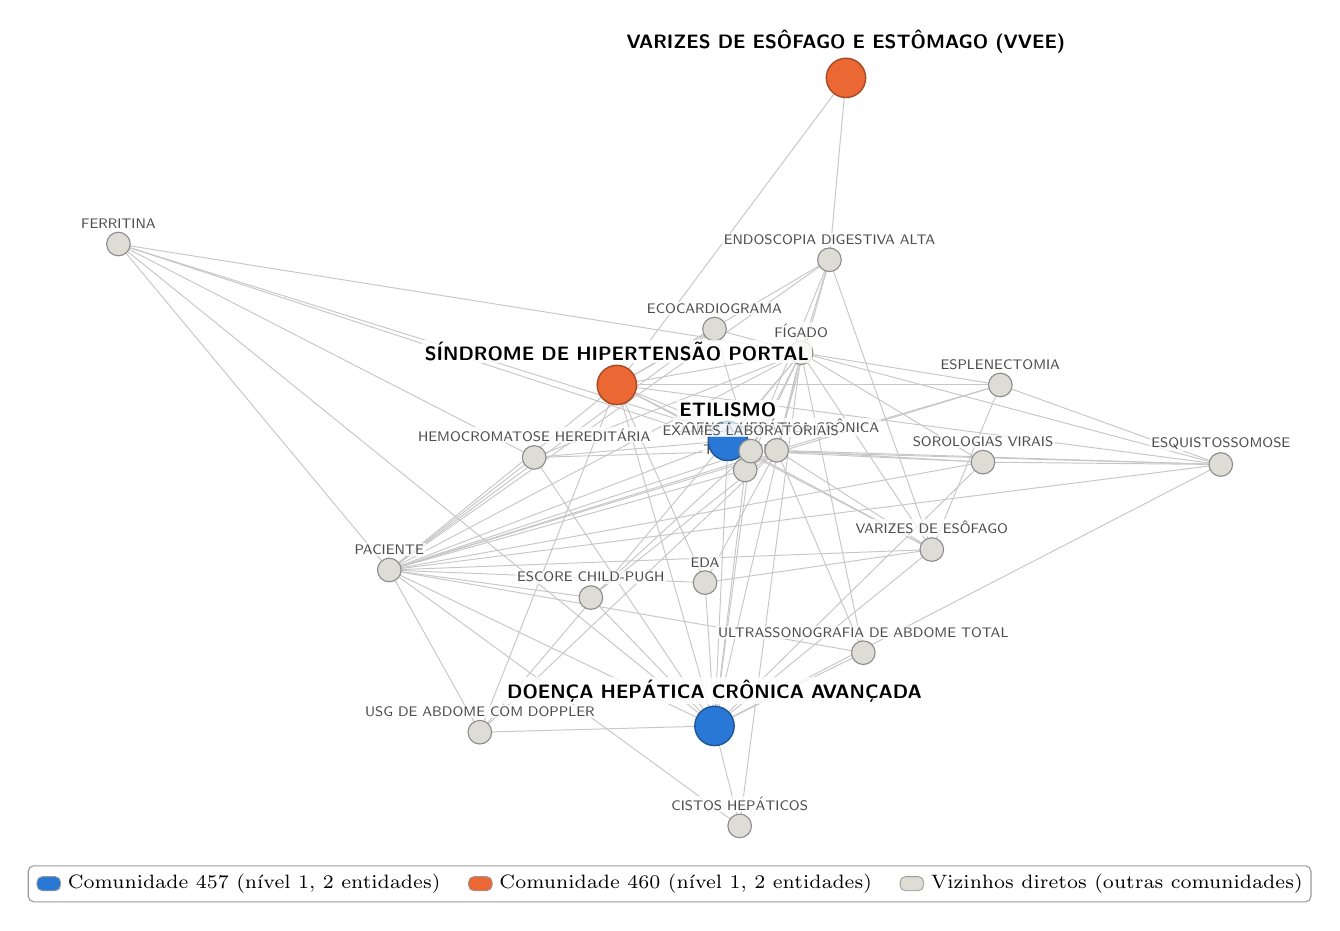
\begin{tikzpicture}[x=1cm, y=1cm]
\draw[black!22, line width=0.35pt] (14.00,4.59) -- (3.44,3.25);
\draw[black!22, line width=0.35pt] (14.00,4.59) -- (8.03,4.76);
\draw[black!22, line width=0.35pt] (14.00,4.59) -- (8.67,6.01);
\draw[black!22, line width=0.35pt] (14.00,4.59) -- (8.36,4.77);
\draw[black!22, line width=0.35pt] (14.00,4.59) -- (11.20,5.60);
\draw[black!22, line width=0.35pt] (14.00,4.59) -- (7.57,1.27);
\draw[black!22, line width=0.35pt] (14.00,4.59) -- (6.33,5.60);
\draw[black!22, line width=0.35pt] (14.00,4.59) -- (10.98,4.62);
\draw[black!22, line width=0.35pt] (5.28,4.68) -- (0.00,7.39);
\draw[black!22, line width=0.35pt] (5.28,4.68) -- (8.67,6.01);
\draw[black!22, line width=0.35pt] (5.28,4.68) -- (7.57,1.27);
\draw[black!22, line width=0.35pt] (5.28,4.68) -- (3.44,3.25);
\draw[black!22, line width=0.35pt] (5.28,4.68) -- (7.74,4.89);
\draw[black!22, line width=0.35pt] (5.28,4.68) -- (8.36,4.77);
\draw[black!22, line width=0.35pt] (9.24,9.50) -- (6.33,5.60);
\draw[black!22, line width=0.35pt] (9.24,9.50) -- (9.03,7.19);
\draw[black!22, line width=0.35pt] (7.96,4.52) -- (3.44,3.25);
\draw[black!22, line width=0.35pt] (7.96,4.52) -- (8.67,6.01);
\draw[black!22, line width=0.35pt] (7.96,4.52) -- (8.03,4.76);
\draw[black!22, line width=0.35pt] (7.96,4.52) -- (7.57,1.27);
\draw[black!22, line width=0.35pt] (7.96,4.52) -- (7.74,4.89);
\draw[black!22, line width=0.35pt] (7.96,4.52) -- (8.36,4.77);
\draw[black!22, line width=0.35pt] (7.89,0.00) -- (8.67,6.01);
\draw[black!22, line width=0.35pt] (7.89,0.00) -- (3.44,3.25);
\draw[black!22, line width=0.35pt] (7.89,0.00) -- (7.57,1.27);
\draw[black!22, line width=0.35pt] (7.74,4.89) -- (7.57,1.27);
\draw[black!22, line width=0.35pt] (7.74,4.89) -- (3.44,3.25);
\draw[black!22, line width=0.35pt] (7.74,4.89) -- (8.67,6.01);
\draw[black!22, line width=0.35pt] (7.74,4.89) -- (8.36,4.77);
\draw[black!22, line width=0.35pt] (7.74,4.89) -- (6.33,5.60);
\draw[black!22, line width=0.35pt] (7.74,4.89) -- (10.33,3.51);
\draw[black!22, line width=0.35pt] (7.74,4.89) -- (8.03,4.76);
\draw[black!22, line width=0.35pt] (0.00,7.39) -- (8.67,6.01);
\draw[black!22, line width=0.35pt] (0.00,7.39) -- (3.44,3.25);
\draw[black!22, line width=0.35pt] (0.00,7.39) -- (8.03,4.76);
\draw[black!22, line width=0.35pt] (0.00,7.39) -- (8.36,4.77);
\draw[black!22, line width=0.35pt] (0.00,7.39) -- (7.57,1.27);
\draw[black!22, line width=0.35pt] (10.33,3.51) -- (9.03,7.19);
\draw[black!22, line width=0.35pt] (10.33,3.51) -- (6.33,5.60);
\draw[black!22, line width=0.35pt] (10.33,3.51) -- (7.45,3.09);
\draw[black!22, line width=0.35pt] (10.33,3.51) -- (8.36,4.77);
\draw[black!22, line width=0.35pt] (10.33,3.51) -- (7.57,1.27);
\draw[black!22, line width=0.35pt] (10.33,3.51) -- (3.44,3.25);
\draw[black!22, line width=0.35pt] (10.33,3.51) -- (8.67,6.01);
\draw[black!22, line width=0.35pt] (10.33,3.51) -- (11.20,5.60);
\draw[black!22, line width=0.35pt] (8.67,6.01) -- (3.44,3.25);
\draw[black!22, line width=0.35pt] (8.67,6.01) -- (8.03,4.76);
\draw[black!22, line width=0.35pt] (8.67,6.01) -- (9.46,2.20);
\draw[black!22, line width=0.35pt] (8.67,6.01) -- (10.98,4.62);
\draw[black!22, line width=0.35pt] (8.67,6.01) -- (7.57,1.27);
\draw[black!22, line width=0.35pt] (8.67,6.01) -- (8.36,4.77);
\draw[black!22, line width=0.35pt] (8.67,6.01) -- (6.33,5.60);
\draw[black!22, line width=0.35pt] (8.67,6.01) -- (11.20,5.60);
\draw[black!22, line width=0.35pt] (8.67,6.01) -- (7.57,6.31);
\draw[black!22, line width=0.35pt] (8.67,6.01) -- (4.59,1.19);
\draw[black!22, line width=0.35pt] (8.67,6.01) -- (9.03,7.19);
\draw[black!22, line width=0.35pt] (7.57,6.31) -- (3.44,3.25);
\draw[black!22, line width=0.35pt] (7.57,6.31) -- (8.03,4.76);
\draw[black!22, line width=0.35pt] (7.57,6.31) -- (6.33,5.60);
\draw[black!22, line width=0.35pt] (6.33,5.60) -- (3.44,3.25);
\draw[black!22, line width=0.35pt] (6.33,5.60) -- (7.57,1.27);
\draw[black!22, line width=0.35pt] (6.33,5.60) -- (8.36,4.77);
\draw[black!22, line width=0.35pt] (6.33,5.60) -- (11.20,5.60);
\draw[black!22, line width=0.35pt] (6.33,5.60) -- (9.03,7.19);
\draw[black!22, line width=0.35pt] (6.33,5.60) -- (7.45,3.09);
\draw[black!22, line width=0.35pt] (6.33,5.60) -- (4.59,1.19);
\draw[black!22, line width=0.35pt] (3.44,3.25) -- (10.98,4.62);
\draw[black!22, line width=0.35pt] (3.44,3.25) -- (8.03,4.76);
\draw[black!22, line width=0.35pt] (3.44,3.25) -- (7.45,3.09);
\draw[black!22, line width=0.35pt] (3.44,3.25) -- (9.03,7.19);
\draw[black!22, line width=0.35pt] (3.44,3.25) -- (8.36,4.77);
\draw[black!22, line width=0.35pt] (3.44,3.25) -- (4.59,1.19);
\draw[black!22, line width=0.35pt] (3.44,3.25) -- (7.57,1.27);
\draw[black!22, line width=0.35pt] (3.44,3.25) -- (11.20,5.60);
\draw[black!22, line width=0.35pt] (3.44,3.25) -- (9.46,2.20);
\draw[black!22, line width=0.35pt] (3.44,3.25) -- (6.00,2.90);
\draw[black!22, line width=0.35pt] (6.00,2.90) -- (7.57,1.27);
\draw[black!22, line width=0.35pt] (6.00,2.90) -- (8.36,4.77);
\draw[black!22, line width=0.35pt] (6.00,2.90) -- (8.03,4.76);
\draw[black!22, line width=0.35pt] (7.57,1.27) -- (8.03,4.76);
\draw[black!22, line width=0.35pt] (7.57,1.27) -- (7.45,3.09);
\draw[black!22, line width=0.35pt] (7.57,1.27) -- (10.98,4.62);
\draw[black!22, line width=0.35pt] (7.57,1.27) -- (4.59,1.19);
\draw[black!22, line width=0.35pt] (7.57,1.27) -- (9.46,2.20);
\draw[black!22, line width=0.35pt] (9.03,7.19) -- (8.03,4.76);
\draw[black!22, line width=0.35pt] (9.03,7.19) -- (8.36,4.77);
\draw[black!22, line width=0.35pt] (7.45,3.09) -- (8.36,4.77);
\draw[black!22, line width=0.35pt] (8.36,4.77) -- (8.03,4.76);
\draw[black!22, line width=0.35pt] (8.36,4.77) -- (9.46,2.20);
\draw[black!22, line width=0.35pt] (8.36,4.77) -- (10.98,4.62);
\draw[black!22, line width=0.35pt] (8.36,4.77) -- (11.20,5.60);
\draw[black!22, line width=0.35pt] (8.36,4.77) -- (4.59,1.19);
\draw[black!22, line width=0.35pt] (8.03,4.76) -- (10.98,4.62);
\node[circle, minimum size=3mm, inner sep=0pt, fill=vNeutro, draw=black!45, line width=0.4pt] (n0) at (14.00,4.59) {};
\node[font=\sffamily\fontsize{5.5}{6.5}\selectfont, text=black!70, fill=white, fill opacity=0.75, text opacity=1, inner sep=0.6pt, anchor=south] at (14.00,4.76) {ESQUISTOSSOMOSE};
\node[circle, minimum size=3mm, inner sep=0pt, fill=vNeutro, draw=black!45, line width=0.4pt] (n1) at (5.28,4.68) {};
\node[font=\sffamily\fontsize{5.5}{6.5}\selectfont, text=black!70, fill=white, fill opacity=0.75, text opacity=1, inner sep=0.6pt, anchor=south] at (5.28,4.85) {HEMOCROMATOSE HEREDITÁRIA};
\node[circle, minimum size=5mm, inner sep=0pt, fill=vLaranja, draw=vLaranja!70!black, line width=0.5pt] (n2) at (9.24,9.50) {};
\node[font=\sffamily\scriptsize\bfseries, fill=white, fill opacity=0.8, text opacity=1, inner sep=1pt, anchor=south] at (9.24,9.77) {VARIZES DE ESÔFAGO E ESTÔMAGO (VVEE)};
\node[circle, minimum size=3mm, inner sep=0pt, fill=vNeutro, draw=black!45, line width=0.4pt] (n3) at (7.96,4.52) {};
\node[font=\sffamily\fontsize{5.5}{6.5}\selectfont, text=black!70, fill=white, fill opacity=0.75, text opacity=1, inner sep=0.6pt, anchor=south] at (7.96,4.69) {TABAGISMO};
\node[circle, minimum size=3mm, inner sep=0pt, fill=vNeutro, draw=black!45, line width=0.4pt] (n4) at (7.89,0.00) {};
\node[font=\sffamily\fontsize{5.5}{6.5}\selectfont, text=black!70, fill=white, fill opacity=0.75, text opacity=1, inner sep=0.6pt, anchor=south] at (7.89,0.17) {CISTOS HEPÁTICOS};
\node[circle, minimum size=5mm, inner sep=0pt, fill=vAzul, draw=vAzul!70!black, line width=0.5pt] (n5) at (7.74,4.89) {};
\node[font=\sffamily\scriptsize\bfseries, fill=white, fill opacity=0.8, text opacity=1, inner sep=1pt, anchor=south] at (7.74,5.16) {ETILISMO};
\node[circle, minimum size=3mm, inner sep=0pt, fill=vNeutro, draw=black!45, line width=0.4pt] (n6) at (0.00,7.39) {};
\node[font=\sffamily\fontsize{5.5}{6.5}\selectfont, text=black!70, fill=white, fill opacity=0.75, text opacity=1, inner sep=0.6pt, anchor=south] at (0.00,7.56) {FERRITINA};
\node[circle, minimum size=3mm, inner sep=0pt, fill=vNeutro, draw=black!45, line width=0.4pt] (n7) at (10.33,3.51) {};
\node[font=\sffamily\fontsize{5.5}{6.5}\selectfont, text=black!70, fill=white, fill opacity=0.75, text opacity=1, inner sep=0.6pt, anchor=south] at (10.33,3.68) {VARIZES DE ESÔFAGO};
\node[circle, minimum size=3mm, inner sep=0pt, fill=vNeutro, draw=black!45, line width=0.4pt] (n8) at (8.67,6.01) {};
\node[font=\sffamily\fontsize{5.5}{6.5}\selectfont, text=black!70, fill=white, fill opacity=0.75, text opacity=1, inner sep=0.6pt, anchor=south] at (8.67,6.18) {FÍGADO};
\node[circle, minimum size=3mm, inner sep=0pt, fill=vNeutro, draw=black!45, line width=0.4pt] (n9) at (7.57,6.31) {};
\node[font=\sffamily\fontsize{5.5}{6.5}\selectfont, text=black!70, fill=white, fill opacity=0.75, text opacity=1, inner sep=0.6pt, anchor=south] at (7.57,6.48) {ECOCARDIOGRAMA};
\node[circle, minimum size=5mm, inner sep=0pt, fill=vLaranja, draw=vLaranja!70!black, line width=0.5pt] (n10) at (6.33,5.60) {};
\node[font=\sffamily\scriptsize\bfseries, fill=white, fill opacity=0.8, text opacity=1, inner sep=1pt, anchor=south] at (6.33,5.87) {SÍNDROME DE HIPERTENSÃO PORTAL};
\node[circle, minimum size=3mm, inner sep=0pt, fill=vNeutro, draw=black!45, line width=0.4pt] (n11) at (3.44,3.25) {};
\node[font=\sffamily\fontsize{5.5}{6.5}\selectfont, text=black!70, fill=white, fill opacity=0.75, text opacity=1, inner sep=0.6pt, anchor=south] at (3.44,3.42) {PACIENTE};
\node[circle, minimum size=3mm, inner sep=0pt, fill=vNeutro, draw=black!45, line width=0.4pt] (n12) at (6.00,2.90) {};
\node[font=\sffamily\fontsize{5.5}{6.5}\selectfont, text=black!70, fill=white, fill opacity=0.75, text opacity=1, inner sep=0.6pt, anchor=south] at (6.00,3.07) {ESCORE CHILD-PUGH};
\node[circle, minimum size=5mm, inner sep=0pt, fill=vAzul, draw=vAzul!70!black, line width=0.5pt] (n13) at (7.57,1.27) {};
\node[font=\sffamily\scriptsize\bfseries, fill=white, fill opacity=0.8, text opacity=1, inner sep=1pt, anchor=south] at (7.57,1.54) {DOENÇA HEPÁTICA CRÔNICA AVANÇADA};
\node[circle, minimum size=3mm, inner sep=0pt, fill=vNeutro, draw=black!45, line width=0.4pt] (n14) at (9.03,7.19) {};
\node[font=\sffamily\fontsize{5.5}{6.5}\selectfont, text=black!70, fill=white, fill opacity=0.75, text opacity=1, inner sep=0.6pt, anchor=south] at (9.03,7.36) {ENDOSCOPIA DIGESTIVA ALTA};
\node[circle, minimum size=3mm, inner sep=0pt, fill=vNeutro, draw=black!45, line width=0.4pt] (n15) at (7.45,3.09) {};
\node[font=\sffamily\fontsize{5.5}{6.5}\selectfont, text=black!70, fill=white, fill opacity=0.75, text opacity=1, inner sep=0.6pt, anchor=south] at (7.45,3.26) {EDA};
\node[circle, minimum size=3mm, inner sep=0pt, fill=vNeutro, draw=black!45, line width=0.4pt] (n16) at (8.36,4.77) {};
\node[font=\sffamily\fontsize{5.5}{6.5}\selectfont, text=black!70, fill=white, fill opacity=0.75, text opacity=1, inner sep=0.6pt, anchor=south] at (8.36,4.94) {DOENÇA HEPÁTICA CRÔNICA};
\node[circle, minimum size=3mm, inner sep=0pt, fill=vNeutro, draw=black!45, line width=0.4pt] (n17) at (4.59,1.19) {};
\node[font=\sffamily\fontsize{5.5}{6.5}\selectfont, text=black!70, fill=white, fill opacity=0.75, text opacity=1, inner sep=0.6pt, anchor=south] at (4.59,1.36) {USG DE ABDOME COM DOPPLER};
\node[circle, minimum size=3mm, inner sep=0pt, fill=vNeutro, draw=black!45, line width=0.4pt] (n18) at (8.03,4.76) {};
\node[font=\sffamily\fontsize{5.5}{6.5}\selectfont, text=black!70, fill=white, fill opacity=0.75, text opacity=1, inner sep=0.6pt, anchor=south] at (8.03,4.93) {EXAMES LABORATORIAIS};
\node[circle, minimum size=3mm, inner sep=0pt, fill=vNeutro, draw=black!45, line width=0.4pt] (n19) at (10.98,4.62) {};
\node[font=\sffamily\fontsize{5.5}{6.5}\selectfont, text=black!70, fill=white, fill opacity=0.75, text opacity=1, inner sep=0.6pt, anchor=south] at (10.98,4.79) {SOROLOGIAS VIRAIS};
\node[circle, minimum size=3mm, inner sep=0pt, fill=vNeutro, draw=black!45, line width=0.4pt] (n20) at (9.46,2.20) {};
\node[font=\sffamily\fontsize{5.5}{6.5}\selectfont, text=black!70, fill=white, fill opacity=0.75, text opacity=1, inner sep=0.6pt, anchor=south] at (9.46,2.37) {ULTRASSONOGRAFIA DE ABDOME TOTAL};
\node[circle, minimum size=3mm, inner sep=0pt, fill=vNeutro, draw=black!45, line width=0.4pt] (n21) at (11.20,5.60) {};
\node[font=\sffamily\fontsize{5.5}{6.5}\selectfont, text=black!70, fill=white, fill opacity=0.75, text opacity=1, inner sep=0.6pt, anchor=south] at (11.20,5.77) {ESPLENECTOMIA};
\node[anchor=north, font=\scriptsize, draw=black!40, line width=0.4pt, rounded corners=2pt, inner sep=3pt] at (7.00,-0.5) {\chip{vAzul}Comunidade 457 (nível 1, 2 entidades)\hspace{10pt}\chip{vLaranja}Comunidade 460 (nível 1, 2 entidades)\hspace{10pt}\chip{vNeutro}Vizinhos diretos (outras comunidades)};
\end{tikzpicture}
}
\caption[Subgrafo do paciente A, por comunidade]{Subgrafo do paciente A, com destaque para as comunidades de nível 1 457 e 460.}
\label{fig:res-subgrafo-paciente-a}
\par\smallskip{\footnotesize Fonte: elaborado pelo autor, com leiaute calculado pela biblioteca NetworkX.}
\end{figure}

A Figura~\ref{fig:res-maiores-grafos} generaliza a observação, comparando os seis maiores subgrafos entre os 537 prontuários da amostra, nos quais as entidades de um mesmo paciente se distribuem por 45 a 63 comunidades distintas, e a Figura~\ref{fig:res-estrutura-agregada} resume estatisticamente a estrutura dos subgrafos de todos os pacientes com dado disponível no índice (536 de 537). O número de entidades e o número de relações por prontuário são fortemente correlacionados ($r=0,959$), com mediana de 38 entidades e 81 relações por paciente, e cada paciente tem suas entidades distribuídas, em média, por comunidades que correspondem a 55\% do número de entidades -- ou seja, a fragmentação entre comunidades observada no caso do paciente A não é um evento isolado, mas uma característica estrutural recorrente do índice. Os resumos das dez comunidades de nível 1 com maior número de relações, que ilustram o conteúdo efetivamente consultado pelos modos \textit{global} e \textit{drift}, são reproduzidos no Apêndice~\ref{ap:comunidades}.

A literatura recente aponta duas causas convergentes para esse quadro, uma em cada etapa da indexação. Na extração, \citet{ye2026} observaram que \textit{prompts} genéricos aplicados a prontuários multiplicam as entidades, ao tratar cada parâmetro laboratorial como entidade independente, e mitigaram o problema exigindo uma única entidade de paciente por registro, à qual se vinculam diagnósticos, medicamentos e exames, princípio que atacaria diretamente a dispersão observada aqui. No agrupamento, \citet{hossain2026} demonstram que, em grafos de conhecimento esparsos, a partição de Leiden não é reprodutível e tende a produzir comunidades de tamanho muito desigual, como as da Tabela~\ref{tab:met-niveis}. Como os resumos de comunidade são o material percorrido pelos modos \textit{global} e \textit{drift}, a granularidade do grafo, definida já na extração de entidades, condiciona diretamente as comunidades formadas pelo Leiden e, por consequência, o contexto disponível a esses modos de busca.

\begin{figure}[!htbp]
\centering
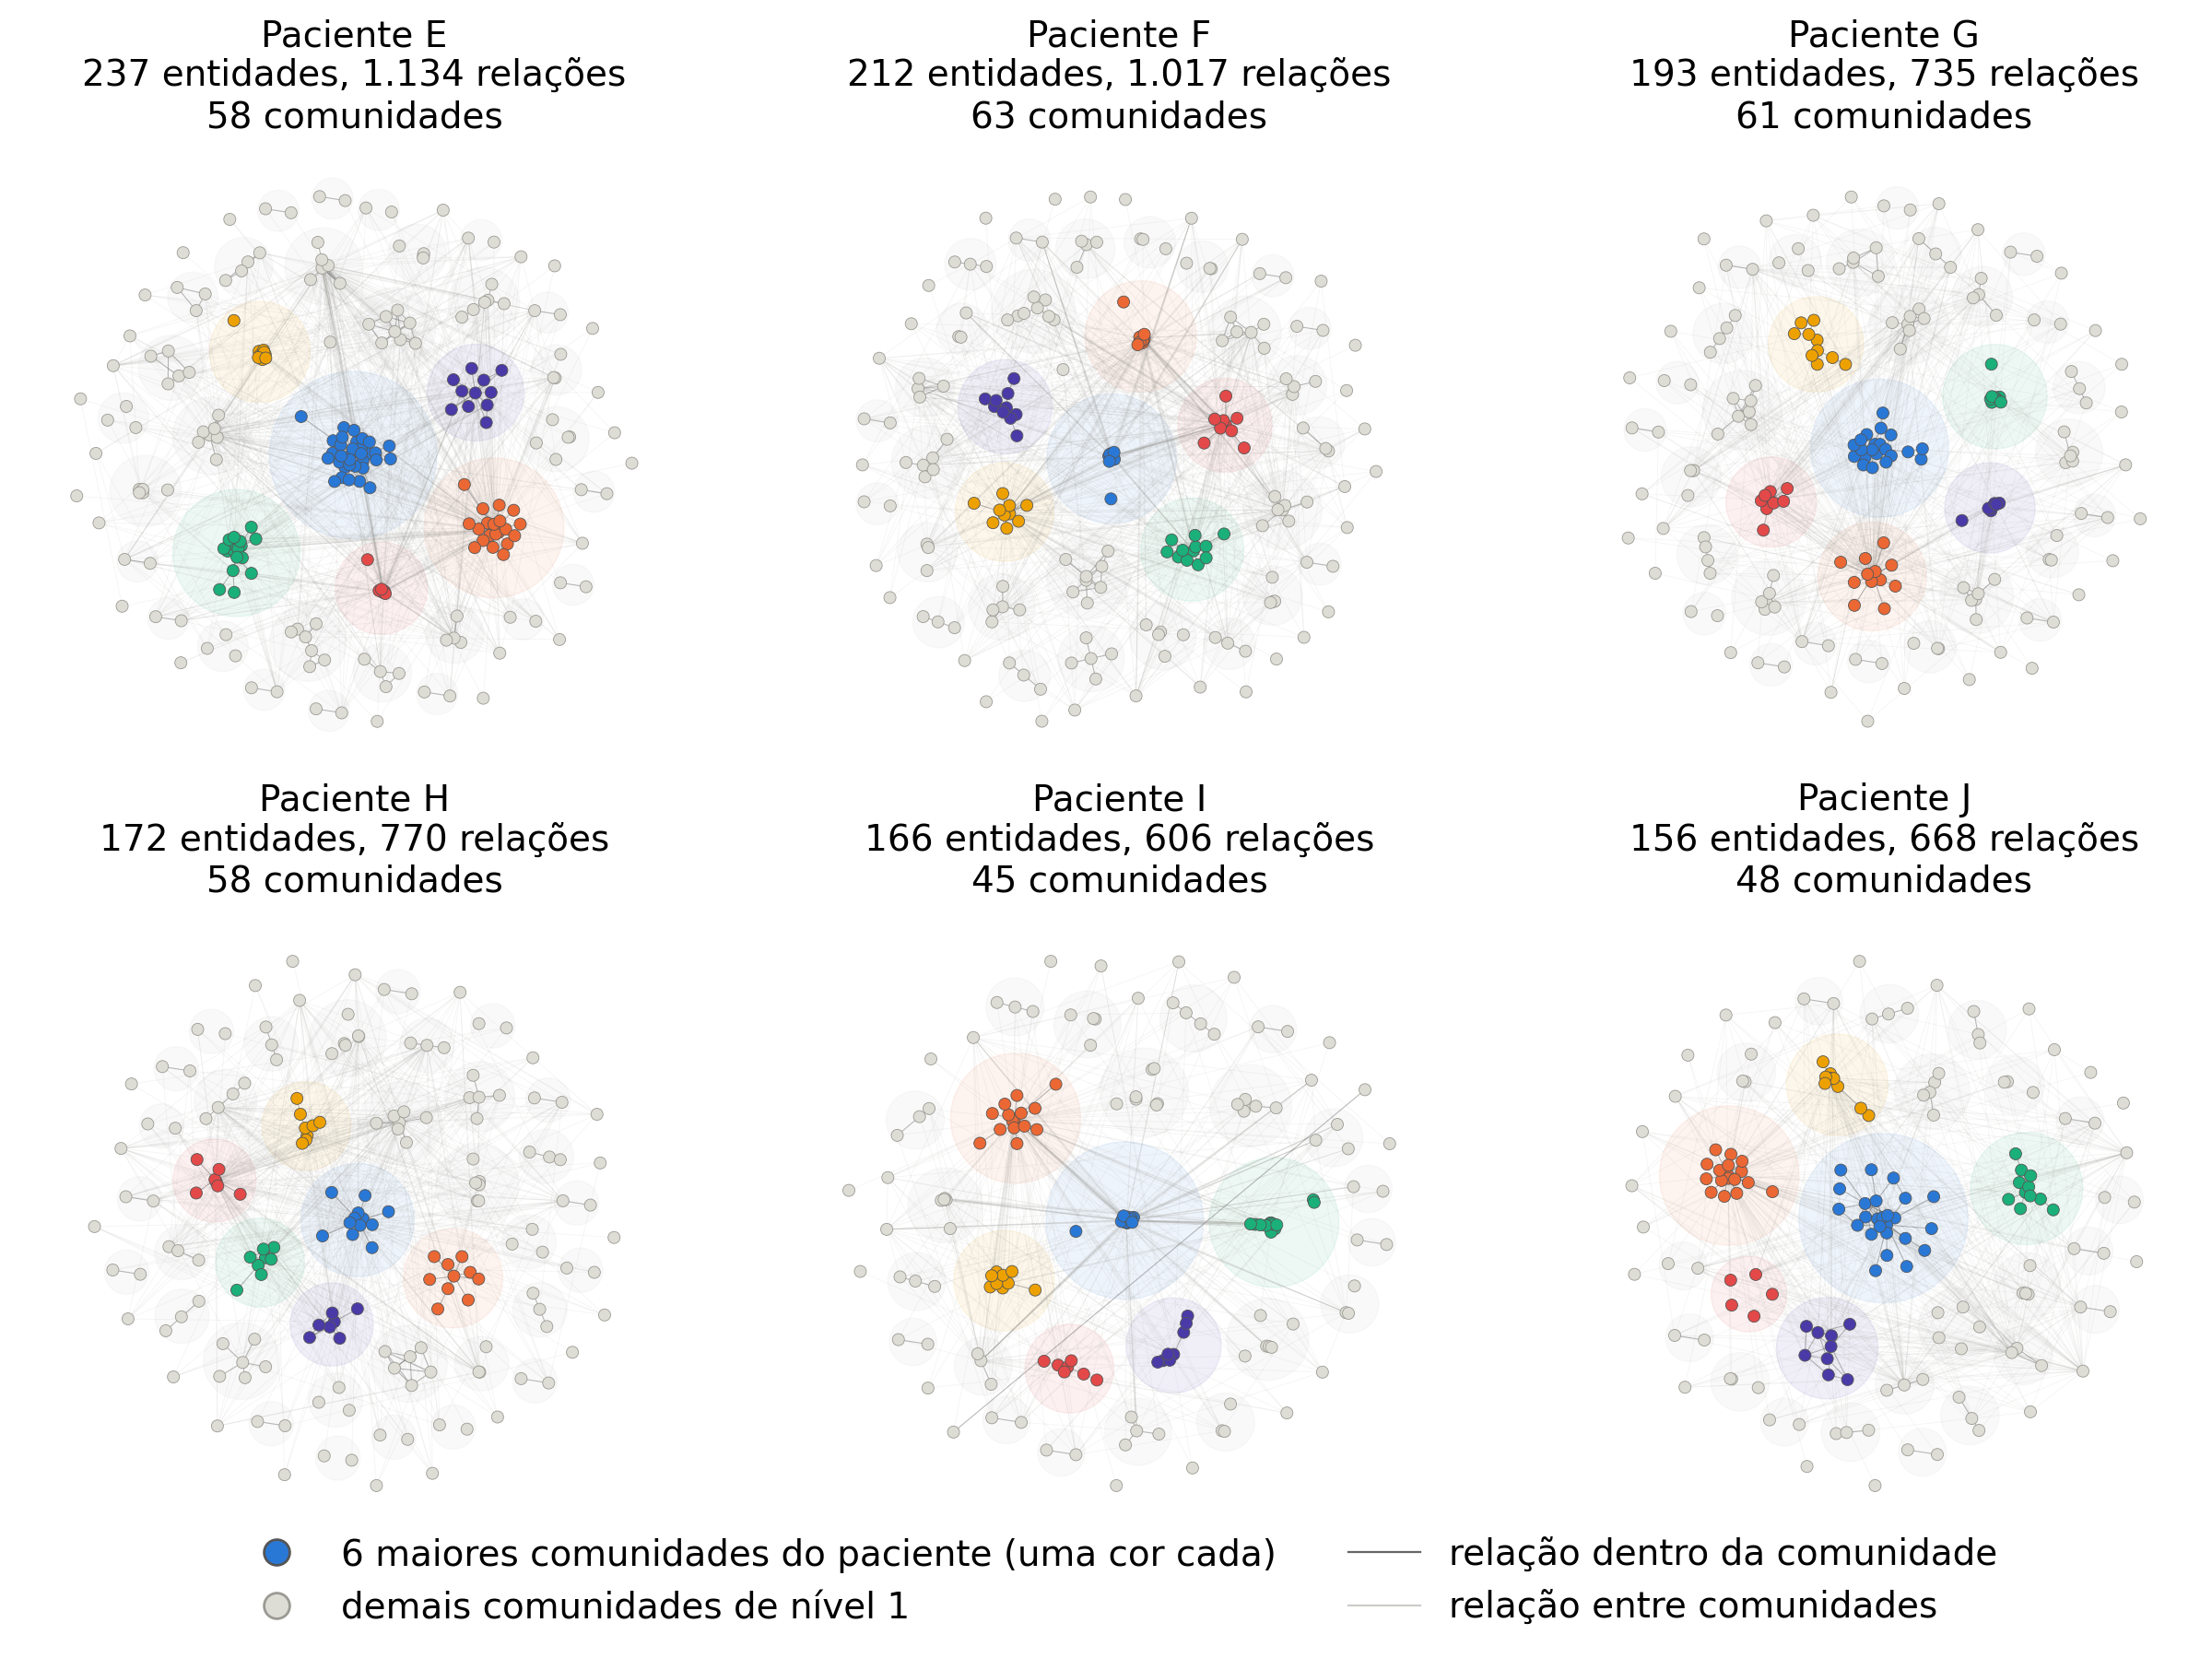
\includegraphics[width=\textwidth]{Cap05/figuras/comparacao_maiores_grafos.png}
\caption[Comparação dos seis maiores subgrafos da amostra]{Os seis maiores subgrafos da amostra, em número de entidades (pacientes E a J), com as entidades agrupadas por comunidade de nível 1; as seis maiores comunidades de cada paciente aparecem em cores, e as demais, em cinza.}
\label{fig:res-maiores-grafos}
\par\smallskip{\footnotesize Fonte: elaborado pelo autor com as bibliotecas NetworkX e matplotlib.}
\end{figure}

\FloatBarrier
\section{Síntese dos resultados}\label{sec:res-sintese}

Em conjunto, os resultados deste capítulo sustentam três conclusões. Primeira, o modo \textit{drift} supera \textit{basic} e \textit{local} em F1 macro, mas o ganho é assimétrico: decorre de uma revocação muito mais alta, e não de maior precisão, de modo que a escolha do sistema deve considerar explicitamente essa troca, e não apenas o valor agregado de F1. Segunda, o ganho do \textit{drift} concentra-se nas doenças que exigem inferência a partir de evidência indireta e dispersa no texto (cirrose, hipertensão portal, esquistossomose), enquanto é marginal nas doenças com marcador textual direto (hepatite B, hepatite C, esteatose), por efeito-teto, e inexistente em HDA, cujo padrão de erro é qualitativamente distinto: confusão anatômica entre sangramento alto e baixo, estatisticamente confirmada. Terceira, a diferença entre os níveis de comunidade 1 e 2 é pequena diante da diferença entre modos de busca: a maior delas, no \textit{drift}, foi de 0,053 de F1 macro, inferior à diferença entre \textit{basic} e \textit{drift} em qualquer dos dois níveis.

\begin{figure}[!htb]
\centering
% Gerado por experiments/grid_search/gera_figuras_tikz_tese.py -- não editar à mão
\begin{tikzpicture}
\begin{groupplot}[
  group style={group size=2 by 2, horizontal sep=1.6cm, vertical sep=1.9cm},
  width=0.5\textwidth, height=5.2cm,
  tick label style={font=\scriptsize}, label style={font=\footnotesize},
  title style={font=\footnotesize\bfseries, yshift=-1mm},
  axis lines=left, axis line style={black!45}, tick style={black!45},
  ymajorgrids, grid style={black!10}, ymin=0,
  /pgf/number format/use comma, /pgf/number format/1000 sep={.},
]
\nextgroupplot[title={Entidades por prontuário}, xlabel={Entidades}, ylabel={Prontuários}]
\addplot[ybar interval, fill opacity=1, draw=white, line width=0.3pt, fill=vAzul] coordinates {(5,12) (12.73,56) (20.47,109) (28.2,77) (35.93,57) (43.67,52) (51.4,39) (59.13,20) (66.87,26) (74.6,11) (82.33,13) (90.07,9) (97.8,14) (105.5,10) (113.3,4) (121,6) (128.7,8) (136.5,2) (144.2,2) (151.9,4) (159.7,1) (167.4,1) (175.1,0) (182.9,0) (190.6,1) (198.3,0) (206.1,1) (213.8,0) (221.5,0) (229.3,1) (237,0)};
\nextgroupplot[title={Relações por prontuário}, xlabel={Relações}, ylabel={Prontuários}]
\addplot[ybar interval, fill opacity=1, draw=white, line width=0.3pt, fill=vLaranja] coordinates {(4,110) (41.67,151) (79.33,76) (117,55) (154.7,30) (192.3,23) (230,12) (267.7,10) (305.3,8) (343,11) (380.7,8) (418.3,8) (456,5) (493.7,7) (531.3,6) (569,7) (606.7,2) (644.3,2) (682,0) (719.7,2) (757.3,1) (795,0) (832.7,0) (870.3,0) (908,0) (945.7,0) (983.3,1) (1021,0) (1059,0) (1096,1) (1134,0)};
\nextgroupplot[title={Entidades $\times$ relações}, xlabel={Entidades}, ylabel={Relações}, xmin=0]
\addplot[only marks, mark=*, mark size=1.1pt, color=vVerde, fill opacity=0.45, draw opacity=0] coordinates {(36,79) (28,48) (56,183) (41,135) (13,23) (37,69) (29,36) (26,31) (40,138) (37,70) (93,420) (106,285) (90,337) (130,527) (85,278) (112,289) (25,95) (17,27) (65,201) (58,136) (63,201) (143,733) (101,438) (56,168) (72,185) (24,48) (193,735) (61,174) (135,594) (24,49) (110,474) (36,61) (73,184) (69,261) (97,358) (45,103) (212,1017) (114,560) (99,499) (69,205) (30,42) (113,472) (49,220) (34,69) (237,1134) (46,80) (32,44) (55,210) (36,79) (103,496) (104,351) (108,412) (128,438) (124,585) (94,358) (110,435) (71,172) (69,230) (166,606) (69,187) (39,142) (55,134) (105,419) (119,487) (45,133) (122,297) (135,594) (124,629) (156,668) (68,158) (129,473) (148,522) (91,293) (131,543) (34,48) (65,141) (113,523) (125,507) (41,93) (31,57) (51,154) (111,448) (74,188) (120,266) (155,546) (41,92) (87,226) (154,533) (67,193) (25,41) (67,197) (76,239) (35,61) (45,78) (38,83) (24,51) (23,45) (19,42) (28,40) (21,33) (16,16) (35,96) (21,45) (30,67) (50,146) (45,180) (61,185) (50,160) (16,11) (35,77) (21,56) (28,39) (28,67) (23,57) (59,179) (34,38) (34,38) (46,135) (63,224) (33,70) (58,135) (49,169) (45,110) (50,87) (10,9) (33,57) (33,57) (53,129) (72,151) (30,77) (23,40) (29,54) (48,122) (41,107) (23,45) (54,142) (26,44) (56,132) (28,43) (28,42) (27,50) (33,44) (61,180) (28,46) (28,52) (19,37) (21,48) (55,136) (62,201) (43,104) (47,79) (19,46) (34,56) (26,53) (48,136) (19,34) (38,73) (41,93) (31,69) (51,195) (24,43) (32,72) (24,62) (32,47) (17,30) (22,23) (21,44) (31,62) (27,64) (21,42) (19,44) (38,58) (19,41) (32,81) (79,217) (19,28) (25,46) (20,38) (41,115) (21,44) (39,103) (40,97) (13,19) (25,35) (21,37) (32,64) (28,33) (22,42) (53,102) (52,115) (47,128) (50,134) (10,9) (27,63) (49,154) (35,92) (53,90) (25,74) (32,53) (27,61) (26,60) (43,130) (17,48) (25,35) (25,35) (52,189) (68,215) (24,50) (34,102) (59,151) (21,31) (24,76) (29,48) (83,250) (41,147) (30,59) (29,65) (45,73) (25,68) (18,23) (18,21) (41,114) (32,71) (17,19) (5,4) (21,25) (9,5) (29,36) (23,35) (30,102) (56,144) (18,29) (35,76) (34,70) (22,39) (54,139) (32,53) (50,153) (24,49) (36,81) (30,80) (59,174) (31,54) (21,32) (37,90) (42,108) (17,22) (27,65) (26,52) (16,20) (31,93) (23,36) (45,97) (14,15) (27,36) (26,45) (57,168) (16,18) (16,18) (13,8) (27,59) (27,59) (29,39) (27,51) (38,68) (45,99) (15,23) (42,85) (13,11) (47,103) (32,30) (30,49) (7,9) (68,260) (30,66) (16,25) (21,40) (21,40) (18,31) (47,82) (66,149) (47,99) (21,35) (23,82) (44,151) (25,42) (18,46) (25,24) (29,44) (53,136) (20,20) (37,85) (44,92) (30,52) (27,48) (13,15) (45,102) (18,17) (8,7) (20,45) (25,59) (20,26) (29,41) (42,78) (32,53) (9,8) (21,25) (49,104) (31,42) (18,16) (38,82) (64,182) (12,11) (39,81) (39,113) (30,50) (31,74) (29,75) (40,79) (40,79) (45,80) (23,40) (44,75) (29,45) (26,44) (48,92) (31,82) (14,23) (51,129) (25,48) (20,45) (13,20) (23,54) (41,158) (29,76) (33,77) (52,134) (43,135) (28,40) (28,46) (29,78) (47,147) (28,86) (56,218) (19,19) (16,17) (49,117) (17,23) (19,40) (20,32) (26,43) (22,32) (21,29) (27,58) (18,31) (33,84) (16,20) (10,13) (58,207) (20,26) (34,56) (22,39) (23,63) (22,29) (10,13) (56,149) (37,86) (28,34) (29,58) (102,366) (78,284) (53,121) (98,348) (43,71) (51,140) (100,395) (97,326) (34,52) (68,156) (94,343) (71,193) (63,169) (23,47) (38,57) (73,133) (12,13) (35,69) (27,78) (36,56) (100,357) (32,64) (85,392) (45,69) (22,28) (35,53) (35,102) (23,29) (155,387) (46,112) (82,361) (131,592) (25,26) (94,311) (74,209) (52,137) (31,73) (60,145) (172,770) (50,123) (95,420) (48,157) (81,308) (83,293) (73,251) (42,79) (31,55) (39,102) (16,20) (82,392) (34,46) (67,174) (100,272) (16,23) (62,111) (102,466) (42,103) (66,215) (62,171) (47,86) (87,315) (41,131) (41,101) (28,51) (26,90) (53,130) (43,100) (87,449) (41,67) (32,62) (61,165) (66,210) (36,67) (73,176) (85,407) (24,54) (57,81) (117,316) (49,135) (73,226) (107,385) (43,73) (31,104) (134,544) (43,87) (49,166) (146,520) (55,149) (82,315) (111,555) (124,616) (136,577) (26,47) (100,578) (40,69) (52,122) (80,302) (46,94) (67,179) (58,127) (27,77) (85,240) (56,149) (41,98) (33,85) (79,355) (71,211) (32,74) (81,389) (68,266) (38,105) (61,182) (31,60) (20,30) (87,352) (24,60) (24,27) (90,317) (65,204) (44,128) (32,84) (52,88) (20,36) (99,283) (19,19) (31,59) (60,125) (45,102) (14,16) (69,250) (17,28) (27,38) (42,85) (95,246) (54,106) (51,133) (143,654) (25,54) (39,74) (25,69) (45,137) (42,98) (26,38) (8,10) (26,61) (27,45) (32,81) (21,32) (53,91) (36,84) (23,40) (45,75) (103,350) (57,94) (88,201) (75,252) (13,13) (59,137) (54,149) (32,44) (24,29) (28,95) (24,38) (18,18) (44,97) (22,32) (26,47)};
\node[anchor=north west, font=\scriptsize, fill=white, inner sep=2pt] at (rel axis cs:0.03,0.97) {$r = 0{,}959$};
\nextgroupplot[title={Comunidades distintas por prontuário}, xlabel={Comunidades distintas (nível 1)}, ylabel={Prontuários}]
\addplot[ybar interval, fill opacity=1, draw=white, line width=0.3pt, fill=vRoxo] coordinates {(0,1) (1,0) (2,0) (3,0) (4,0) (5,2) (6,3) (7,3) (8,5) (9,6) (10,9) (11,18) (12,16) (13,24) (14,16) (15,29) (16,27) (17,21) (18,26) (19,30) (20,20) (21,22) (22,15) (23,23) (24,21) (25,19) (26,13) (27,10) (28,12) (29,14) (30,6) (31,19) (32,8) (33,11) (34,8) (35,6) (36,10) (37,8) (38,5) (39,9) (40,2) (41,3) (42,5) (43,3) (44,4) (45,3) (46,2) (47,1) (48,3) (49,2) (50,0) (51,3) (52,3) (53,0) (54,1) (55,0) (56,0) (57,1) (58,2) (59,0) (60,1) (61,1) (62,0) (63,1) (64,0)};
\end{groupplot}
\end{tikzpicture}

\caption[Distribuição estrutural dos subgrafos por prontuário]{Entidades, relações e comunidades por prontuário, e correlação entre entidades e relações.}
\label{fig:res-estrutura-agregada}
\par\smallskip{\footnotesize Fonte: elaborado pelo autor a partir do índice construído.}
\end{figure}

\cleardoublepage
% % % % % % % % % % % % % % % % % % % % % % % % % % % %
\chapter{Conclusão}\label{cap:conclusao}

Este trabalho avaliou o GraphRAG como abordagem para a identificação de doenças hepáticas em prontuários eletrônicos reais, escritos em português brasileiro, no ambulatório de hepatologia do Hospital Universitário da Universidade Federal de Alagoas. A avaliação comparou quatro modos de busca do Microsoft GraphRAG (\textit{basic}, \textit{local}, \textit{global} e \textit{drift}), em dois níveis de granularidade da hierarquia de comunidades, sobre uma amostra de 537 prontuários com rótulo de referência anotado por especialista, para oito doenças hepáticas de interesse clínico. Até onde os trabalhos revisados no Capítulo~\ref{cap:relacionados} permitem afirmar, esta é a primeira avaliação do GraphRAG sobre prontuários clínicos reais em português brasileiro com esse desenho: \textit{ground truth} humano, comparação sistemática entre modos de busca e níveis de comunidade, e investigação estatística dos mecanismos de acerto e erro.

O resultado central é que o modo \textit{drift} obtém o maior F1 macro entre os sistemas comparáveis, mas esse ganho não decorre de maior exatidão: decorre de uma revocação substancialmente mais alta, da ordem de 95\% contra 60\% a 67\% dos demais modos, obtida ao custo de uma precisão inferior. Essa troca não se distribui igualmente entre as oito doenças. Nas condições que exigem inferência a partir de evidência dispersa no texto, como cirrose hepática e hipertensão portal, o \textit{drift} supera o modo \textit{basic} por margens expressivas, de quase 20 pontos de F1. Nas condições com marcador textual direto, como esteatose hepática e hepatite C, o ganho é pequeno, por efeito de teto; na hepatite B e, de forma mais acentuada, na hemorragia digestiva alta, o \textit{drift} sequer supera os modos mais simples, e análises estatísticas dirigidas confirmaram um mecanismo concreto de confusão anatômica entre sangramento alto e baixo como explicação para esse último caso. Quanto à granularidade da hierarquia de comunidades, o teste de McNemar exato não encontrou diferença estatisticamente significativa entre os dois níveis avaliados, em nenhum dos modos de busca comparáveis, o que indica que essa escolha de projeto é, dentro da faixa testada, menos determinante para o desempenho do que a escolha do modo de busca em si.

Esses achados respondem à pergunta de pesquisa enunciada no Capítulo~\ref{cap:introducao} de forma que qualifica, mais do que confirma, a expectativa inicial de que um modo de busca mais elaborado produziria resultados uniformemente melhores. O GraphRAG, e em particular o modo \textit{drift}, mostra-se mais adequado quanto mais indireta for a evidência que sustenta o diagnóstico, e menos vantajoso, podendo até ser contraproducente, quando a doença já possui um marcador textual objetivo e inequívoco. Essa qualificação tem valor prático direto para quem for aplicar GraphRAG a tarefas semelhantes de extração clínica: a escolha do modo de busca deve ser orientada pela natureza da evidência textual disponível para cada classe, e não assumida de forma genérica a partir do desempenho agregado de um único sistema.

\section{Contribuições}\label{sec:conc-contribuicoes}

As principais contribuições deste trabalho são:

\begin{itemize}
    \item uma avaliação sistemática do Microsoft GraphRAG sobre prontuários clínicos reais em português brasileiro, com \textit{ground truth} anotado por especialista, preenchendo uma lacuna identificada na revisão de trabalhos relacionados (Capítulo~\ref{cap:relacionados});
    \item um funil de construção de amostra e de rótulos de referência, por triagem textual, triagem por LLM e anotação manual, que torna viável avaliar oito classes com prevalência desigual sem recorrer a uma amostra aleatória simples;
    \item a caracterização estatística, por meio dos testes de McNemar, U de Mann-Whitney e qui-quadrado, dos mecanismos que explicam tanto os casos em que o modo \textit{drift} acerta onde os demais erram quanto o inverso, confirmando formalmente, entre outros achados, a confusão anatômica entre hemorragia digestiva alta e sangramento baixo;
    \item uma taxonomia qualitativa dos padrões de erro do \textit{drift}, com casos concretos de negação textual ignorada, confusão entre diagnóstico de familiar e do próprio paciente, confusão entre marcador de imunidade vacinal e infecção ativa, e ao menos um caso de citação de resultado de exame inexistente no texto-fonte;
    \item um conjunto de \textit{scripts} e um \textit{pipeline} de avaliação reutilizáveis, que cobrem desde a triagem da amostra até a análise estatística e qualitativa dos resultados, disponíveis para extensão em trabalhos futuros no mesmo domínio.
\end{itemize}

\section{Limitações}\label{sec:conc-limitacoes}

Os resultados devem ser interpretados à luz das limitações detalhadas na Seção~\ref{sec:met-limitacoes}. Em síntese, destacam-se: a variância de latência e de custo introduzida pelo modelo de raciocínio híbrido utilizado na tentativa de validação do \textit{prompt} reforçado para hemorragia digestiva alta, que impediu a conclusão dessa validação dentro de prazo razoável; a insuficiência estatística da classe de peritonite bacteriana espontânea, com apenas dois casos positivos na amostra; o caráter não aleatório da amostra, enriquecida por triagem textual, que impede a leitura da prevalência observada como estimativa epidemiológica; a impossibilidade de concluir, com o modelo adotado, uma avaliação confiável dos sistemas do modo \textit{global}; e a dependência dos resultados por nível de comunidade de uma única realização da partição de Leiden, cuja estabilidade entre indexações não foi avaliada.

\section{Trabalhos Futuros}\label{sec:conc-futuros}

A partir dos resultados e das limitações identificadas, propõem-se as seguintes direções para trabalhos futuros:

\begin{itemize}
    \item concluir a validação do \textit{prompt} reforçado para hemorragia digestiva alta (Seção~\ref{sec:res-validacao-hda}), hoje inconclusiva por limitações de infraestrutura, preferencialmente sobre um modelo de linguagem sem o custo de latência observado no modelo de raciocínio híbrido utilizado neste trabalho;
    \item avaliar os sistemas do modo \textit{global} (S5 e S6) com um modelo ou uma configuração que não incorra no volume excessivo de chamadas observado na seleção dinâmica de comunidades, de modo a completar a comparação entre os quatro modos de busca do GraphRAG;
    \item investigar correções específicas para os falsos positivos de hepatite B e hepatite C descritos na Seção~\ref{sec:res-investigacao-erro}, como regras explícitas de distinção entre marcadores de imunidade vacinal e de infecção ativa, e de tratamento de doença resolvida após terapia antiviral;
    \item avaliar \textit{prompts} de indexação com regras explícitas de granularidade, como a exigência de uma única entidade de paciente por registro proposta por \citet{ye2026}, e alternativas determinísticas ao algoritmo de Leiden, como a decomposição em $k$-núcleos \citep{hossain2026}, quanto ao efeito sobre a fragmentação das comunidades e sobre o desempenho dos modos de busca;
    \item estender a avaliação a um segundo anotador humano, de modo a medir a concordância entre anotadores e fortalecer a confiabilidade do \textit{ground truth} para além da anotação única adotada neste trabalho;
    \item replicar o desenho experimental sobre um corpus de outra instituição ou especialidade clínica, para avaliar em que medida os padrões de acerto e erro aqui identificados são específicos deste ambulatório ou generalizáveis a outros contextos de texto clínico em português.
\end{itemize}

\cleardoublepage
%%% % % % % % % % % % % % % % % % % % % % % % % % % % %
%%% % % % % % % % % % % % % % % % % % % % % % % % % % %
% \markright{Bibliography}
%\renewcommand\bibname{Bibliography}


% % % % % % % % % % % % % % % % % % % % % % % % % % %
% Definir estilo bibliográfico  % % % % % % % % % % %
% % % % % % % % % % % % % % % % % % % % % % % % % % %
\label{sec:sampleReferences}

% o estilo myheadings não atualiza o cabeçalho no \chapter* da bibliografia; sem esta
% marca, as páginas das referências herdavam a última seção ("Trabalhos Futuros")
\markboth{\bibname}{\bibname}

% \bibliography (natbib/BibTeX) já imprime a bibliografia neste ponto do documento --
% \printbibliography é um comando do biblatex, pacote nunca carregado aqui (só natbib,
% ver main.tex). Misturar os dois gerava "Undefined control sequence" no fim do
% documento. Corrigido em 2026-11-02.
% \nocite{*} também foi removido: listava no PDF final toda entrada do .bib, mesmo as
% não citadas no texto -- mantenha-o comentado a menos que isso seja intencional.
\bibliography{Ref/SampleReferences} % arquivo .bib


% % % % % % % % % % % % % % % % % % % % % % % % % % %
% Apêndices  % % % % % % % % % % % % % % % % % % % %
% % % % % % % % % % % % % % % % % % % % % % % % % % %
\cleardoublepage
\appendix
\chapter{\texorpdfstring{\textit{Prompt}}{Prompt} de Extração de Entidades e Relações}\label{ap:prompt-indexacao}

Este apêndice reproduz o \textit{prompt} de extração de entidades e relações empregado na indexação do corpus, gerado pelo procedimento automático de ajuste de \textit{prompts} do GraphRAG (Seção~\ref{sec:met-prompt-tuning}). As instruções são apresentadas na íntegra, em inglês, tal como geradas pela ferramenta. As expressões entre chaves, como \texttt{\{tuple\_delimiter\}}, \texttt{\{record\_delimiter\}}, \texttt{\{completion\_delimiter\}} e \texttt{\{input\_text\}}, são variáveis substituídas pelo GraphRAG no momento de cada chamada ao modelo.

O \textit{prompt} original continha três exemplos \textit{few-shot} que o ajuste automático extraiu de trechos do próprio corpus. Para preservar a confidencialidade dos dados, esses exemplos foram substituídos por um único exemplo fictício, redigido no mesmo estilo dos prontuários e no mesmo formato de saída.

\begin{small}
\VerbatimInput[breaklines, breakanywhere, fontsize=\footnotesize, frame=single, framesep=2mm, rulecolor=\color{black!40}]{Apendices/prompt_extracao_grafo.txt}
\end{small}

\chapter{\texorpdfstring{\textit{Prompt}}{Prompt} de Consulta}\label{ap:prompt-consulta}

Este apêndice reproduz na íntegra o \textit{prompt} de extração multirrótulo enviado em cada consulta, descrito na Seção~\ref{sec:met-prompt} e empregado em todos os sistemas avaliados. As expressões entre chaves são substituídas, a cada consulta, pelo número do prontuário e pelo texto do prontuário, truncado em 8.000 caracteres.

\begin{small}
\VerbatimInput[breaklines, breakanywhere, fontsize=\footnotesize, frame=single, framesep=2mm, rulecolor=\color{black!40}]{Apendices/prompt_consulta_multilabel.txt}
\end{small}

\chapter{\texorpdfstring{\textit{Prompt}}{Prompt} da Triagem por LLM}\label{ap:prompt-triagem}

Este apêndice reproduz o \textit{prompt} empregado na segunda etapa do funil de construção da amostra, a triagem por LLM (Seção~\ref{sec:met-amostra}). Para cada prontuário candidato, a lista de condições é preenchida com as doenças sinalizadas pela triagem por expressões regulares, e o modelo responde, para cada uma, se há evidência clara de sua presença. As expressões entre chaves são substituídas, a cada chamada, pelo número do prontuário, pelas condições candidatas e pelo texto do prontuário, truncado em 8.000 caracteres.

\begin{small}
\VerbatimInput[breaklines, breakanywhere, fontsize=\footnotesize, frame=single, framesep=2mm, rulecolor=\color{black!40}]{Apendices/prompt_triagem_llm.txt}
\end{small}

\chapter{Dicionários de Termos e Marcadores}\label{ap:dicionarios}

Este apêndice reúne os dicionários empregados na triagem por expressões regulares (Seção~\ref{sec:met-amostra}) e na extração determinística das respostas (Seção~\ref{sec:met-parser}). Todos os termos e marcadores são aplicados ao texto normalizado, em letras minúsculas e sem acentos, razão pela qual aparecem nessa forma. Os nomes das doenças e seus sinônimos são procurados como palavras inteiras; os marcadores de negação, incerteza e contexto histórico são buscados em qualquer posição da linha, e alguns deles são expressões regulares.

A Tabela~\ref{tab:ap-marcadores} lista os marcadores que descartam uma menção: na triagem, a negação, a incerteza e, para HDA e PBE, o contexto histórico; no \textit{parser}, a negação, com marcadores adicionais incorporados após auditorias de falsos positivos. A Tabela~\ref{tab:ap-termos} lista os termos reconhecidos para cada doença, compartilhados pela triagem e pelo \textit{parser}.

\begin{table}[H]
\centering
\caption[Marcadores de negação, incerteza e contexto histórico]{Marcadores que descartam uma menção, na forma normalizada, por etapa em que são aplicados.}
\label{tab:ap-marcadores}
\small
\renewcommand{\arraystretch}{1.25}
\begin{tabular}{@{}>{\raggedright\arraybackslash}p{3.4cm}p{11.2cm}@{}}
\toprule
Marcador & Termos e expressões \\
\midrule
Negação (triagem e \textit{parser}) & \raggedright \texttt{ausente}, \texttt{ausencia}, \texttt{descartad}, \texttt{exclu}, \texttt{negativ}, \texttt{nao\ confirmad}, \texttt{nao\ evidenciad}, \texttt{sem\ evidencia}, \texttt{nao\ ha\ evidencia}, \texttt{negado}, \texttt{nao\ documentad}, \texttt{nao\ presente}, \texttt{nega\ }, \texttt{nego\ }, \texttt{negou\ } \tabularnewline
Negação (só no \textit{parser}) & \raggedright \texttt{\textbackslash{}bnr\textbackslash{}b}, \texttt{nao\ ha\ .\{0,40\}que\ .\{0,15\}confirm}, \texttt{nao\ esta\ documentad}, \texttt{nao\ consta}, \texttt{nao\ ha\ relato} \tabularnewline
Incerteza (triagem) & \raggedright \texttt{a\ esclarecer}, \texttt{a\ definir}, \texttt{a\ investigar}, \texttt{epidemiologia\ positiva}, \texttt{epidemiologia\ para}, \texttt{suspeita\ de}, \texttt{possivel\ }, \texttt{provavel\ }, \texttt{risco\ para}, \texttt{\textbackslash{}?} \tabularnewline
Contexto histórico (triagem, só HDA e PBE) & \raggedright \texttt{passado\ de}, \texttt{historia\ de}, \texttt{historico\ de}, \texttt{previo\ de}, \texttt{previa\ de}, \texttt{antecedente\ de} \tabularnewline
\bottomrule
\end{tabular}
\par\smallskip{\footnotesize Fonte: elaborado pelo autor a partir do código da triagem (\texttt{filtro\_triagem.py}) e do \textit{parser} (\texttt{parser\_doencas.py}).}
\end{table}

\begin{table}[H]
\centering
\caption[Termos reconhecidos para cada doença]{Termos reconhecidos para cada uma das oito doenças, na forma normalizada.}
\label{tab:ap-termos}
\small
\renewcommand{\arraystretch}{1.25}
\begin{tabular}{@{}>{\raggedright\arraybackslash}p{3.4cm}p{11.2cm}@{}}
\toprule
Doença & Termos \\
\midrule
Cirrose hepática & \raggedright \texttt{cirrose}, \texttt{cirrose\ hepatica}, \texttt{cirrose\ hepatica\ descompensada}, \texttt{cirrose\ hepatica\ alcoolica}, \texttt{cirrose\ hepatica\ viral\ c}, \texttt{cirrose\ micronodular}, \texttt{cirrose\ descompensada}, \texttt{cirrose\ hepatica\ cronica} \tabularnewline
Esquistossomose & \raggedright \texttt{esquistossomose}, \texttt{equistossomose}, \texttt{esquistossomose\ hepatoesplenica}, \texttt{esquistossomose\ hepatoesplenica\ (ehe)}, \texttt{esquistossomose\ mansoni}, \texttt{esquistossomose\ mansonica}, \texttt{ehe} \tabularnewline
Hepatite C & \raggedright \texttt{hepatite\ c}, \texttt{hepatite\ c\ (hcv)}, \texttt{hepatite\ c\ cronica}, \texttt{hepatite\ cronica\ viral\ c} \tabularnewline
Hepatite B & \raggedright \texttt{hepatite\ b}, \texttt{hepatite\ b\ (hbv)}, \texttt{hepatite\ b\ cronica}, \texttt{hepatite\ b\ inativa}, \texttt{hepatite\ b\ resolvida}, \texttt{hepatite\ cronica\ b}, \texttt{hepatite\ cronica\ viral\ b}, \texttt{virus\ b\ (hepatite\ b)} \tabularnewline
Esteatose hepática & \raggedright \texttt{esteatose}, \texttt{esteatose\ hepatica}, \texttt{esteatose\ hepatica\ difusa}, \texttt{dhgna}, \texttt{nafld}, \texttt{masld}, \texttt{mash}, \texttt{nash}, \texttt{doenca\ hepatica\ gordurosa\ nao\ alcoolica}, \texttt{doenca\ hepatica\ gordurosa\ nao\ alcoolica\ (dhgna)}, \texttt{doenca\ hepatica\ esteatotica\ metabolica}, \texttt{doenca\ hepatica\ esteatotica\ metabolica\ (mash)}, \texttt{esteato-hepatite\ nao\ alcoolica}, \texttt{esteato-hepatite\ nao\ alcoolica\ (nash)}, \texttt{esteatohepatite}, \texttt{esteatohepatite\ nao\ alcoolica} \tabularnewline
Hipertensão portal & \raggedright \texttt{hipertensao\ portal}, \texttt{hipertensao\ porta}, \texttt{sindrome\ de\ hipertensao\ portal}, \texttt{sindrome\ da\ hipertensao\ portal}, \texttt{hipertensao\ portal\ nao\ cirrotica}, \texttt{ehe/hp} \tabularnewline
Hemorragia digestiva alta & \raggedright \texttt{hda}, \texttt{hemorragia\ digestiva\ alta}, \texttt{hemorragia\ digestiva\ alta\ varicosa}, \texttt{hemorragia\ varicosa} \tabularnewline
Peritonite bacteriana espontânea & \raggedright \texttt{pbe}, \texttt{peritonite\ bacteriana\ espontanea}, \texttt{peritonite\ bacteriana\ espontanea\ (pbe)} \tabularnewline
\bottomrule
\end{tabular}
\par\smallskip{\footnotesize Fonte: elaborado pelo autor a partir do código do \textit{parser} (\texttt{parser\_doencas.py}).}
\end{table}


%%% % % % % % % % % % % % % % % % % % % % % % % % % % %
%%% % % % % % % % % % % % % % % % % % % % % % % % % % %
\end{document}
